\chapter{Introduction: What Empirical IO Studies}\label{ch:intro}

Consider a coffee shop on a university campus. It is the only seller of coffee inside one building, and a few
other cafes operate a short walk away. Does it have market power, and how much? To answer we would like to know
three things. The first is its demand curve, that is, how many cups it would sell at each price. The second is its
marginal cost of a cup. The third is how its rivals would respond if it raised its price. None of the three is
written down anywhere. What we can observe is its price and perhaps the number of cups it sells. Now and then an
event moves one of the unknowns, such as a tax on coffee, a rise in the price of beans or a new cafe next door. Empirical industrial organization is the craft of learning about demand, cost and the conduct of
firms from data of this kind. This chapter introduces that craft, its history and the questions it serves.

The chapter has four movements. \Cref{sec:01-what-is-io,sec:01-definitions} state the questions of the field and
define its basic objects: markets, concentration, the Lerner index and markups. They end with the Cournot model,
which links concentration to margins and so motivates the first empirical program of the field.
\Cref{sec:01-scp,sec:01-scp-econometrics,sec:01-scp-after} study that program, the structure-conduct-performance
paradigm. Its cross-industry regressions of margins on concentration dominated the field for three decades. We
show formally why they cannot separate demand, cost and conduct, and we follow the debates they left behind,
including the recent one over rising markups. \Cref{sec:01-neio,sec:01-identification} present the response, the
New Empirical Industrial Organization of \citet{Bresnahan1989}. It studies one industry at a time, treats conduct
as a parameter, and asks which features of the data identify market power. \Cref{sec:01-today} describes empirical
IO today, following \citet{EinavLevin2010}. Most work now estimates demand, recovers marginal costs from
first-order conditions and simulates counterfactual equilibria. \Cref{sec:01-roadmap} lays out the rest of the book.

The coffee shop returns twice. \Cref{ex:01-coffee} uses an estimated elasticity to infer its marginal cost and shows
how the answer depends on conduct. \Cref{ex:01-coffee-tax} predicts the effect of a tax on its price and shows how
the answer depends on the shape of demand. These two dependencies, on conduct and on functional form, recur in
every chapter. The theory behind this chapter is developed in \cref{ch:theory}, the measurement of conduct in
\cref{ch:conduct}, and the demand models of the structural workflow in \cref{ch:aids,ch:discrete,ch:logit,ch:blp}.
The Cournot, collusion and cross-industry regression models of \cref{sec:01-cournot-hhi,sec:01-endogeneity} are
worked through in full in \cref{app:problems}.

\section{What industrial organization studies}\label{sec:01-what-is-io}

\emph{Industrial organization} (IO) is the field of economics that studies how industries are organized and
how firms and consumers behave within them. In the words of \citet[p.~146]{EinavLevin2010}, the field ``is
concerned with the structure of industries in the economy and the behavior of firms and individuals in these
industries.'' Its distinctive focus is on markets that depart from \emph{perfect competition}, the benchmark
in which many small firms take the price as given and price equals marginal cost. Such departures arise from
scale economies, transaction costs, strategic behavior and other frictions \citep[p.~146]{EinavLevin2010}.

The traditional questions of IO concern competition policy, regulation, and the determinants and consequences
of market power. Competition policy asks, for example, whether a merger will raise prices or whether a group of
sellers is fixing prices. Regulation asks how to set prices and entry rules in industries with large scale
economies, such as electricity transmission or local telephone service. The study of \emph{market power}, the
ability of a firm to keep its price above the competitive level, asks where such power comes from and what it
costs consumers. Each of these questions requires a model of how firms interact. A firm's best price depends on
the prices of its rivals, and a merger changes the incentives of the merging firms and of every firm that
competes with them.

The field therefore looks mostly at what happens between firms. What happens inside a firm, such as how it
organizes production or designs incentives for its employees, belongs largely to other fields. Productivity is
the main exception. Many IO economists measure productivity and study how competition and the selection of
efficient firms shape it. This book does not cover productivity.

Empirical IO relies on economic theory more than most other fields of applied microeconomics. We see two
reasons. The first is that theory has a great deal to say about firms and markets. Firms that set prices every
day plausibly come close to maximizing profit, and profit maximization in equilibrium imposes sharp
restrictions on data. \citet[pp.~158--159]{EinavLevin2010} draw the contrast with research on education.
Standard theory says little about how third graders learn. For firms and markets, they argue, theory ``has a
lot to say and, when appropriately used, generally serves to clarify rather than to complicate one's
understanding of a market.'' The second reason is historical. IO had a head start on the econometric modeling
of strategic behavior. By the late 1980s a body of work already estimated demand, cost and the form of
competition jointly within single industries, and \citet{Bresnahan1989} could survey it. A further
consideration reinforces both reasons. Many IO questions concern events that have not yet happened, such as a
proposed merger, and only a model of the industry can predict their effects.

These tools now travel beyond the traditional boundaries of the field. IO-trained economists study insurers
and hospitals in health care, schools and colleges in education, and banks and lenders in finance. Questions
about competition have become central in each of these sectors. The same methods serve markets with \emph{adverse
selection}, such as insurance, where the customers most eager to buy are the most costly to serve. They also
serve platforms that bring two groups of users together. \citet[p.~149]{EinavLevin2010}
report that the demand models developed in \cref{ch:aids,ch:discrete,ch:logit,ch:blp} have spread into trade,
education, housing, health and environmental economics. Economists sometimes call this expansion ``IO+.'' The
editors of the latest Handbook of Industrial Organization describe the same trend \citep[Preface, p.~xv]{HoHortacsuLizzeri2021}.
In their account, the ``econometric revolution'' that began with the New Empirical Industrial Organization of
\cref{sec:01-neio} has kept maturing. Its toolbox now reaches credit and insurance markets, financial markets, health
care, the energy sector and the environment.

Empirical IO also has a large footprint in policy and business. Its methods are used in merger reviews and
antitrust litigation, in regulatory decisions, in price setting by retailers, and in the design of auctions and
marketplaces \citep[p.~145]{EinavLevin2010}. Antitrust agencies and courts use demand estimates to define
markets, to simulate the price effects of mergers, and to compute damages from excessive prices
\citep[p.~149]{EinavLevin2010}. Around 1980, antitrust arguments often rested on simple concentration measures.
Today the agencies routinely commission econometric studies of the industry under review
\citep[p.~152]{EinavLevin2010}. Welfare measures derived from estimated demand have shaped the debate over how
the Consumer Price Index should account for new goods \citep[p.~149]{EinavLevin2010}. Empirical studies of
bidding have informed the regulation of wholesale electricity markets \citep[p.~154]{EinavLevin2010}. We treat
merger analysis in \cref{ch:mergers}, new goods in \cref{ch:newgoods}, and auctions in
\cref{ch:auction-theory,ch:auction-empirics}.

Almost every question in this book comes back to three objects, which we call the \emph{primitives} of a
market. The first is \emph{demand}, which describes how many units consumers buy at each price and how they
substitute between products. The second is \emph{cost}, in particular the \emph{marginal cost} of producing one
more unit. The third is \emph{conduct}, the way firms compete. Firms may set prices or quantities, act
independently or coordinate, and look ahead to rivals' reactions or ignore them. Price equals marginal cost
plus a markup, and the markup depends on demand and on conduct:
\begin{equation}\label{eq:01-price-decomposition}
  \text{price} = \text{marginal cost} + \text{markup}(\text{demand}, \text{conduct}).
\end{equation}
\Cref{sec:01-lerner,sec:01-cournot-hhi} make this decomposition precise.

In most data sets none of the three primitives is observed directly. We observe prices and quantities, which
are equilibrium outcomes. Each observed pair lies on the demand curve and on the firms' pricing rule at the
same time, so a scatter of prices and quantities traces out neither of them. \Cref{ch:aids,ch:logit} treat
this simultaneity problem. Accounting data record average and historical costs, with overhead allocated by
convention. \citet[p.~151]{EinavLevin2010}, following \citet{Bresnahan1989}, stress that accounting practices
are not designed to report the economic notion of marginal cost. Conduct is recorded nowhere, and firms that
coordinate have every reason to hide it. The history of empirical IO, told in the rest of this chapter, is a
sequence of answers to one problem. How can we learn about demand, cost and conduct from data on prices and
quantities?

\begin{remark}[Scope of this book]
The book covers static imperfect competition and its measurement (\cref{ch:theory,ch:conduct,ch:diffprod}) and
demand estimation and its applications (\cref{ch:aids,ch:discrete,ch:logit,ch:blp,ch:airlines,ch:newgoods}). It
also covers competition policy toward mergers and collusion (\cref{ch:mergers,ch:collusion-theory,ch:collusion-evidence})
and auctions of a single object (\cref{ch:auction-theory,ch:auction-empirics}). It does not treat in depth the
models of entry and market structure, dynamic competition and investment, productivity, vertical relations,
consumer search, or price discrimination. \Cref{sec:01-today} sketches some of these topics, and
\cref{sec:01-roadmap} gives a detailed roadmap.
\end{remark}

\section{Market structure, market power, and markups}\label{sec:01-definitions}

A question in the background of much of empirical IO is how market structure affects market power. Do markets
with fewer or larger firms have higher prices relative to cost? Answering it requires four ingredients, which
this section develops in turn. We need a definition of the market (\cref{sec:01-market-definition}) and a
measure of its structure (\cref{sec:01-concentration}). We also need a measure of market power
(\cref{sec:01-lerner,sec:01-fixed-costs}) and a theory that links structure to market power
(\cref{sec:01-cournot-hhi}).

\subsection{Markets and market definition}\label{sec:01-market-definition}

\begin{definition}[Market]\label{def:01-market}
A \emph{market} is a set of products and a geographic area within which buyers substitute strongly, and from
which they substitute only weakly toward outside products or sellers. The set of products is the
\emph{product market}, and the area is the \emph{geographic market}.
\end{definition}

Market shares, concentration and even the label ``monopoly'' are defined only relative to a market. A firm
that sells the only brand of a particular breakfast cereal has a monopoly over that brand. The same firm has a
modest share of ready-to-eat cereal and a negligible share of all breakfast foods. Every statistic computed
from shares therefore inherits the choice of market.

Sometimes the market is obvious. Cement is heavy and cheap relative to its weight, so a cement plant in an
isolated town competes only with plants within a short trucking distance. The product market is cement, and
the geographic market is the area around the town. Sometimes the market is far from obvious. Online retailers
sell to the whole country and compete with physical stores. Breakfast cereals form a chain of substitutes, from
children's cereals to adult cereals to other breakfast foods, with no natural break. In such cases any boundary
is a judgment call.

Antitrust practice disciplines this judgment with the \emph{hypothetical monopolist test}. We start from a
candidate set of products and an area. We then ask whether a hypothetical profit-maximizing firm that owned all
of them would impose a \emph{small but significant and non-transitory increase in price} (SSNIP), commonly 5
percent. If substitution to products outside the set would make such an increase unprofitable, the set is too
narrow, and we add the next closest substitute. The \emph{relevant market} is the smallest set that passes the
test. The test is a statement about demand elasticities, so it needs the demand models of
\cref{ch:aids,ch:discrete,ch:logit,ch:blp}. \Cref{ch:mergers} develops it, together with the loss of sales that
would make a price increase unprofitable and the concentration thresholds used in merger review.

Some economists doubt that market definition is the right first step at all. \citet[p.~1049]{Bresnahan1989}
notes that antitrust often needs to know whether a group of firms acting together, or a single firm, has market
power. He adds in a footnote that ``these questions are well-posed, even where the usual method of answering
them \ldots{} is senseless'' \citep[p.~1049, n.~44]{Bresnahan1989}. The usual method defines a `relevant
market' and calculates market shares in it. Market power is a property of the demand curve that a firm or group
faces, and we can try to estimate that curve directly. Market definition is a device for approximating the same
object with shares. \Cref{ch:conduct} shows how to estimate the demand curve that a single firm faces after its
rivals respond. This
direct approach is one motivation for the New Empirical Industrial Organization of \cref{sec:01-neio}.

\subsection{Concentration measures}\label{sec:01-concentration}

In empirical work, \emph{market structure} usually means a measure of concentration computed from market
shares. Consider a market with $N$ firms $i = 1, \dots, N$ that sell a homogeneous good. Firm $i$ produces
$q_i$, total output is $Q = \sum_{i=1}^{N} q_i$, and firm $i$'s \emph{market share} is $s_i = \frac{q_i}{Q}$.
Shares are fractions that sum to one. With differentiated products, shares are computed from units or revenues
within the defined market. We write $s_{(1)} \ge s_{(2)} \ge \dots \ge s_{(N)}$ for the shares sorted from
largest to smallest.

\begin{definition}[Concentration measures]\label{def:01-concentration}
\leavevmode
\begin{enumerate}[label=(\roman*)]
  \item The \emph{$m$-firm concentration ratio} is the combined share of the $m$ largest firms,
  \[
    \mathit{CR}_m = \sum_{i=1}^{m} s_{(i)} .
  \]
  \item The \emph{Herfindahl-Hirschman index}, often shortened to the Herfindahl index, is the sum of squared
  shares,
  \begin{equation}\label{eq:01-hhi}
    \HHI = \sum_{i=1}^{N} s_i^2 .
  \end{equation}
  Antitrust agencies report it in \emph{HHI points}, equal to $10{,}000 \times \HHI$, which is the sum of
  squared shares measured in percent.
  \item The \emph{numbers equivalent} is $N^{\mathrm{eq}} = \frac{1}{\HHI}$, the number of equal-sized firms that would
  produce the same index.
\end{enumerate}
\end{definition}

The concentration ratios in common use are $\mathit{CR}_1$ (the share of the largest firm), $\mathit{CR}_3$,
$\mathit{CR}_4$ and $\mathit{CR}_8$. They satisfy $\frac{m}{N} \le \mathit{CR}_m \le 1$ for $m \le N$, because
the average of the $m$ largest shares is at least the average share $\frac{1}{N}$. The Herfindahl-Hirschman index is
named after Orris Herfindahl and Albert Hirschman. It uses every share, and it weights large firms more heavily
because each share is weighted by itself. The next result makes precise what the index measures.

\begin{lemma}[Bounds and variance decomposition]\label{prop:01-hhi-variance}
Let $\sigma_s^2 = \frac{1}{N}\sum_{i=1}^{N} \left(s_i - \frac{1}{N}\right)^2$ be the cross-firm variance of
market shares. Then
\begin{equation}\label{eq:01-hhi-variance}
  \HHI = \frac{1}{N} + N\sigma_s^2 ,
\end{equation}
and $\frac{1}{N} \le \HHI \le 1$. The lower bound holds with equality if and only if all shares are equal. The
upper bound holds with equality if and only if one firm has the whole market.
\end{lemma}

\begin{proof}
The mean share is $\frac{1}{N}\sum_{i} s_i = \frac{1}{N}$, so $\sigma_s^2$ is the variance of shares around
their mean. Expand the sum of squared deviations:
\begin{align*}
  \sum_{i=1}^{N} \left(s_i - \frac{1}{N}\right)^2
  &= \sum_{i=1}^{N} s_i^2 - \frac{2}{N}\sum_{i=1}^{N} s_i + N \cdot \frac{1}{N^2} \\
  &= \HHI - \frac{2}{N} + \frac{1}{N} \\
  &= \HHI - \frac{1}{N}.
\end{align*}
The second line uses $\sum_i s_i = 1$. The left side equals $N\sigma_s^2$, which gives
\eqref{eq:01-hhi-variance}. Because $\sigma_s^2 \ge 0$, we have $\HHI \ge \frac{1}{N}$, with equality if and
only if every share equals $\frac{1}{N}$. For the upper bound, $0 \le s_i \le 1$ implies $s_i^2 \le s_i$, so
$\HHI \le \sum_i s_i = 1$. Equality requires $s_i^2 = s_i$ for every $i$, so every share is zero or one. Since
the shares sum to one, exactly one firm has share one.
\end{proof}

\Cref{prop:01-hhi-variance} shows that the index combines two features of a market. The term $\frac{1}{N}$
reflects the number of firms, and the term $N\sigma_s^2$ reflects the inequality of their sizes. A market with
many firms is highly concentrated if one of them is much larger than the rest. Correspondingly, the numbers
equivalent $N^{\mathrm{eq}}$ lies between $1$ and $N$, and it falls below $N$ whenever shares are unequal.
\Cref{sec:01-demsetz} uses the decomposition to show that cost differences between firms raise concentration
in a Cournot market.

\begin{example}[Two rankings of concentration]\label{ex:01-concentration}
Consider two hypothetical industries. Industry A has one dominant firm with half of the market and 25 small
firms with 2 percent each. Industry B has four firms with 20 percent each and four firms with 5 percent each.
The four-firm concentration ratios are
\begin{align*}
  \mathit{CR}_4^A &= 0.50 + 3 \times 0.02 = 0.56, \\
  \mathit{CR}_4^B &= 4 \times 0.20 = 0.80,
\end{align*}
so this ratio ranks B as more concentrated. The Herfindahl-Hirschman indices are
\begin{align*}
  \HHI^A &= 0.50^2 + 25 \times 0.02^2 = 0.25 + 0.01 = 0.26, \\
  \HHI^B &= 4 \times 0.20^2 + 4 \times 0.05^2 = 0.16 + 0.01 = 0.17,
\end{align*}
or 2,600 and 1,700 HHI points. The index ranks A as more concentrated. The numbers equivalents are
$N^{\mathrm{eq}}_A = \frac{1}{0.26} \approx 3.8$ and $N^{\mathrm{eq}}_B = \frac{1}{0.17} \approx 5.9$. Industry A has 26 firms but is
as concentrated as a market with about four equal firms. In industry B, $N = 8$ and every share deviates from
the mean $\frac{1}{8}$ by $0.075$, so \eqref{eq:01-hhi-variance} confirms the arithmetic:
\[
  \HHI^B = \frac{1}{8} + 8 \times 0.075^2 = 0.125 + 0.045 = 0.17 .
\]
The ratio $\mathit{CR}_4$ ignores how shares are distributed within the top four and among the remaining firms.
The index $\HHI$ responds mostly to the single large firm in A.
\end{example}

\begin{remark}[Which indices are admissible?]\label{rem:01-ej-axioms}
\citet{EncaouaJacquemin1980} ask which functions $R(s_1, \dots, s_N)$ of the shares deserve the name of a
concentration index \citep[Section~5.5]{Tirole1988}. They impose three axioms. The index is symmetric, so that
permuting the shares leaves it unchanged. It satisfies the \emph{Lorenz condition}, which says that a
mean-preserving spread of the shares, moving share toward the tails of their distribution, raises the index.
With symmetric firms it falls as their number grows, so that
$R\left(\frac{1}{N}, \dots, \frac{1}{N}\right) \ge R\left(\frac{1}{N+1}, \dots, \frac{1}{N+1}\right)$. They show
that a family of indices satisfying the axioms takes the form
\begin{equation}\label{eq:01-ej-family}
  R(s_1, \dots, s_N) = \sum_{i=1}^{N} s_i\, h(s_i) ,
\end{equation}
where $h$ is nondecreasing and $s\,h(s)$ is convex. The Herfindahl-Hirschman index has $h(s) = s$. The
\emph{entropy index} $\sum_i s_i \ln s_i$ has $h(s) = \ln s$, and it equals $-\ln N$ when $N$ firms are equal. The
ratio $\mathit{CR}_m$ satisfies the axioms, yet it does not belong to the family.

Two steps show why every member of the family satisfies the axioms. Let $g(s) = s\,h(s)$. With equal shares,
$R = N g\left(\frac{1}{N}\right) = h\left(\frac{1}{N}\right)$, which cannot rise with $N$ because $h$ is
nondecreasing. For the Lorenz condition, move the share $\Delta > 0$ from firm $j$ to a firm $i$ with
$s_i \ge s_j$. This transfer is the elementary step of a mean-preserving spread. The index changes by
\[
  \left[g(s_i + \Delta) - g(s_i)\right] - \left[g(s_j) - g(s_j - \Delta)\right] \ge 0 .
\]
The inequality holds because the slope of a convex function over an interval of length $\Delta$ rises as the
interval moves to the right. For the Herfindahl index the change is $2\Delta(s_i - s_j) + 2\Delta^2 > 0$. The
ratio $\mathit{CR}_m$ meets the Lorenz condition only weakly, since a transfer between two firms outside the top
$m$ can leave it unchanged.
\end{remark}

\begin{remark}[What concentration measures leave out]\label{rem:01-concentration-limits}
A concentration index summarizes shares and nothing else. It ignores how close the products of different firms
are as substitutes, whether firms have spare capacity, how easily new firms can enter, and whether buyers are
large enough to bargain. Market structure in the broad sense includes the number of sellers and buyers,
vertical integration, and product differentiation. Differentiation is \emph{vertical} when all buyers rank the
products the same way, as with quality grades. It is \emph{horizontal} when buyers rank them differently, as
with flavors or locations. No single index captures all of these features. \citet[p.~283]{BakerBresnahan1988}
give an example from US brewing over 1962--1982. Pabst and Coors had similar national market shares, yet
their estimates show that Pabst was virtually a price taker while Coors had substantial market power.

Shares are also used mechanically in merger review. If firms $i$ and $j$ merge and the merged firm keeps the
combined share $s_i + s_j$, the index rises by
\[
  (s_i + s_j)^2 - s_i^2 - s_j^2 = 2 s_i s_j .
\]
Oligopoly theory does not guarantee that the merged firm keeps the combined share, so this calculation is only
a first screen (\cref{ch:theory,ch:mergers}).
\end{remark}

\subsection{Market power, markups, and the Lerner index}\label{sec:01-lerner}

The competitive benchmark is price equal to marginal cost. A firm that takes the market price as given expands
output until its marginal cost reaches the price. Market power is the ability to do better than this, and we
measure it by the gap between price and marginal cost.

\begin{definition}[Market power and markups]\label{def:01-market-power}
A firm has \emph{market power} if it can profitably set its price above the competitive level, which is its
marginal cost $mc$. For a firm that charges the price $p$, we use four measures of the gap between price and
marginal cost.
\begin{enumerate}[label=(\roman*)]
  \item The \emph{Lerner index} is $L = \frac{p - mc}{p}$, the margin as a fraction of price
  \citep{Lerner1934}.
  \item The \emph{markup ratio} is $\mu = \frac{p}{mc}$.
  \item The \emph{markup rate} is $\mu - 1 = \frac{p - mc}{mc}$, the margin as a fraction of marginal cost.
  \item The \emph{dollar markup} is $p - mc$.
\end{enumerate}
\end{definition}

In this chapter $\mu$ always denotes the markup ratio. Later chapters use $\mu_{ijt}$ for the consumer-specific
part of utility, and the context keeps the two apart. The recent literature on markups, including
\citet{DeLoeckerEeckhoutUnger2020}, reports the ratio $\mu$. The Lerner index and the markup ratio carry the
same information:
\begin{align}
  L = \frac{p - mc}{p} &= 1 - \frac{mc}{p} \notag\\
  &= 1 - \frac{1}{\mu} \notag\\
  &= \frac{\mu - 1}{\mu} . \label{eq:01-lerner-mu}
\end{align}
Inverting gives $\mu = \frac{1}{1 - L}$. When $0 < mc \le p$, the Lerner index lies in $[0, 1]$ and
$\mu \ge 1$. Price taking gives $L = 0$ and $\mu = 1$. A markup rate of 50 percent, or $\mu = 1.5$, corresponds
to $L = \frac{0.5}{1.5} = \frac{1}{3}$.

The basic theory of how a firm with market power sets its price fits in one proposition. We state it for a firm
that faces a \emph{residual demand} curve $Q(p)$, the quantity it sells at each of its own prices once we
account for what its rivals do. For a monopolist, residual demand is market demand.

\begin{proposition}[The pricing rule]\label{prop:01-pricing-rule}
A firm faces a twice differentiable residual demand $Q(p)$ with $Q(p) > 0$ and $Q'(p) < 0$, and it produces
at constant marginal cost $c > 0$. Let $p$ be an interior maximizer of profit $\pi(p) = (p - c)Q(p)$. Then the
following hold at $p$.
\begin{enumerate}[label=(\roman*)]
  \item The dollar markup equals the reciprocal of the \emph{semi-elasticity} of demand
  $-\frac{\dd \ln Q(p)}{\dd p}$:
  \begin{equation}\label{eq:01-dollar-markup}
    p - c = m \equiv -\frac{Q(p)}{Q'(p)}, \qquad -\frac{\dd \ln Q(p)}{\dd p} = -\frac{Q'(p)}{Q(p)} = \frac{1}{m}.
  \end{equation}
  \item The Lerner index equals the reciprocal of the residual demand elasticity
  $\varepsilon^R = -Q'(p)\frac{p}{Q(p)}$:
  \begin{equation}\label{eq:01-lerner-rule}
    \frac{p - c}{p} = \frac{1}{\varepsilon^R} .
  \end{equation}
  \item Price is a multiple of marginal cost,
  \begin{equation}\label{eq:01-price-multiple}
    p = \frac{\varepsilon^R}{\varepsilon^R - 1}\, c ,
  \end{equation}
  and the residual elasticity exceeds one, $\varepsilon^R > 1$.
\end{enumerate}
The second-order condition is $\pi''(p) = 2Q'(p) + (p - c)Q''(p) \le 0$.
\end{proposition}

\begin{proof}
Differentiate profit with respect to price:
\[
  \pi'(p) = Q(p) + (p - c)Q'(p).
\]
At an interior maximum the first-order condition holds:
\begin{equation}\label{eq:01-foc-monopoly}
  Q'(p)(p - c) + Q(p) = 0 .
\end{equation}
For (i), divide \eqref{eq:01-foc-monopoly} by $-Q'(p) > 0$ and rearrange:
\begin{align*}
  -(p - c) - \frac{Q(p)}{Q'(p)} &= 0, \\
  p - c &= -\frac{Q(p)}{Q'(p)} = m .
\end{align*}
The semi-elasticity is $-\frac{\dd \ln Q}{\dd p} = -\frac{Q'(p)}{Q(p)}$, which is $\frac{1}{m}$ by definition of
$m$. For (ii), divide both sides of (i) by $p$:
\[
  \frac{p - c}{p} = -\frac{Q(p)}{p\,Q'(p)} = \frac{1}{-Q'(p)\frac{p}{Q(p)}} = \frac{1}{\varepsilon^R} .
\]
For (iii), multiply (ii) by $p$ and collect the terms in $p$:
\begin{align*}
  p - c &= \frac{p}{\varepsilon^R}, \\
  p\left(1 - \frac{1}{\varepsilon^R}\right) &= c, \\
  p &= \frac{\varepsilon^R}{\varepsilon^R - 1}\, c .
\end{align*}
The first line shows that $p > c > 0$, because $Q > 0$ and $Q' < 0$ make $\varepsilon^R > 0$. The ratio
$\frac{p}{c} = \frac{\varepsilon^R}{\varepsilon^R - 1}$ must then exceed one. If $\varepsilon^R < 1$ the ratio
would be negative, and $\varepsilon^R = 1$ would make the second line read $0 = c$. Hence $\varepsilon^R > 1$.
The second-order condition is the requirement that $\pi''(p) \le 0$ at a maximum.
\end{proof}

The two arrangements (i) and (ii) are the formulas used most often in this book. Arrangement (i) says that the
markup in dollars equals the inverse of the semi-elasticity, the proportional fall in quantity per dollar of
price increase. Arrangement (ii), often called the \emph{Lerner equation} or the \emph{inverse elasticity rule},
says that the markup as a fraction of price equals the inverse of the elasticity. A firm prices further above
cost when its customers respond less to price. Both formulas involve only the residual demand curve of the firm
itself, evaluated at the chosen price. The same logic carries over to the models of price competition with
differentiated products that dominate modern work. There, each firm's price equals its marginal cost plus a
markup that depends on the semi-elasticity of its own demand \citep[p.~151]{EinavLevin2010}. Statement (iii) adds that a firm with market power never prices where
its residual demand is inelastic. At such a price, a small price increase would raise revenue and lower cost.

Two demand curves show the difference between the arrangements. With constant-elasticity demand
$Q(p) = A p^{-\varepsilon^R}$, the Lerner index is the constant $\frac{1}{\varepsilon^R}$, so price is a fixed
multiple of cost. With exponential demand $Q(p) = A e^{-\frac{p}{b}}$, the semi-elasticity is the constant
$\frac{1}{b}$, so the dollar markup is the constant $b$ whatever the cost. \Cref{ch:theory} develops these cases
and their implications for how cost changes pass through to prices.

\begin{remark}[Residual versus market demand]\label{rem:01-residual}
In an oligopoly the residual elasticity $\varepsilon^R$ differs from the \emph{market elasticity}
$\varepsilon = -\frac{\dd Q}{\dd p}\frac{p}{Q}$ of total industry demand. Customers who leave one firm may buy
from a rival instead of leaving the market, so a firm typically faces more elastic demand than the industry as a
whole. A simple case makes this precise. Suppose $N$ firms sell a homogeneous good with inverse market demand
$P(Q)$, and firm $i$ takes its rivals' total output $Q_{-i} = Q - q_i$ as fixed. The firm's inverse residual
demand is then $P(q_i + Q_{-i})$, whose slope in $q_i$ is $P'(Q)$. Since the slope of demand is the reciprocal
of the slope of inverse demand, the market elasticity is $\varepsilon = -\frac{P(Q)}{Q P'(Q)}$. The residual
elasticity of firm $i$ is therefore
\begin{equation}\label{eq:01-residual-elasticity}
  \varepsilon^R_i = -\frac{P(Q)}{q_i P'(Q)} = \frac{Q}{q_i}\left(-\frac{P(Q)}{Q P'(Q)}\right)
  = \frac{\varepsilon}{s_i} .
\end{equation}
A firm with a 25 percent share faces a residual elasticity four times the market elasticity.
\Cref{sec:01-cournot-hhi} returns to this case. \Cref{ch:conduct} shows how \citet{BakerBresnahan1988}
estimate residual demand curves directly, and \cref{ch:diffprod} treats firms that sell several differentiated
products.
\end{remark}

\Cref{prop:01-pricing-rule} can be run in reverse. If we know the elasticity of the demand that a firm faces
and we observe its price, the pricing rule tells us its marginal cost.

\begin{corollary}[Inferring marginal cost from prices]\label{prop:01-infer-cost}
Suppose we observe the price $p$ of a firm that maximizes profit as in \cref{prop:01-pricing-rule}, and we have
an estimate $\hat\varepsilon^R$ of its residual demand elasticity at that price. Then the Lerner index and
marginal cost are estimated by
\begin{equation}\label{eq:01-infer-cost}
  \hat L = \frac{1}{\hat\varepsilon^R}, \qquad
  \hat c = p + \frac{Q(p)}{\hat Q'(p)} = p\left(1 - \frac{1}{\hat\varepsilon^R}\right).
\end{equation}
If $\hat\varepsilon^R$ has standard error $\mathrm{se}(\hat\varepsilon^R)$ and $p$ is measured without error,
the delta method gives the approximate standard errors
\begin{equation}\label{eq:01-infer-cost-se}
  \mathrm{se}(\hat c) \approx \frac{p}{(\hat\varepsilon^R)^2}\,\mathrm{se}(\hat\varepsilon^R), \qquad
  \mathrm{se}(\hat L) \approx \frac{1}{(\hat\varepsilon^R)^2}\,\mathrm{se}(\hat\varepsilon^R).
\end{equation}
\end{corollary}

\begin{proof}
Solving (i) of \cref{prop:01-pricing-rule} for $c$ gives $c = p + \frac{Q(p)}{Q'(p)}$. Solving (ii) gives
$c = p\left(1 - \frac{1}{\varepsilon^R}\right)$. Replacing the unknown slope or elasticity with its estimate
gives \eqref{eq:01-infer-cost}. For the standard errors, write $\hat c = g(\hat\varepsilon^R)$ with
$g(\varepsilon) = p - \frac{p}{\varepsilon}$. Its derivative is
\[
  g'(\varepsilon) = \frac{p}{\varepsilon^2} .
\]
Let $\varepsilon^R_0$ be the true elasticity. A first-order Taylor expansion gives
$\hat c - c \approx g'(\varepsilon^R_0)\left(\hat\varepsilon^R - \varepsilon^R_0\right)$, so
\[
  \Var(\hat c) \approx \left(\frac{p}{(\varepsilon^R_0)^2}\right)^2 \Var(\hat\varepsilon^R) .
\]
Taking square roots and evaluating the derivative at the estimate gives the first formula in
\eqref{eq:01-infer-cost-se}. The same steps with $h(\varepsilon) = \frac{1}{\varepsilon}$, whose derivative is
$h'(\varepsilon) = -\frac{1}{\varepsilon^2}$, give the second. \Cref{app:econometrics} states the delta method
in general.
\end{proof}

This inversion runs through the rest of the book. \citet{Rosse1970} used it to estimate the cost functions of
newspapers ``without using cost data,'' as his title puts it. \citet[p.~151]{EinavLevin2010} describe it as the
standard way to recover costs in modern work when cost data are unavailable or unreliable. The inversion rests
on a maintained assumption, namely that the firm maximizes profit under a known form of conduct. If firms
compete differently, the same price and elasticity imply a different cost. With the industry \emph{conduct
parameter} $\theta$, which we introduce in \cref{sec:01-cournot-hhi} and develop in
\cref{sec:01-conduct-parameter}, the inversion becomes
\begin{equation}\label{eq:01-infer-cost-theta}
  \hat c = p + \theta\,\frac{Q(p)}{\hat Q'(p)} = p\left(1 - \frac{\theta}{\hat\varepsilon}\right),
\end{equation}
where $Q$ and $\hat\varepsilon$ now refer to market demand. Monopoly corresponds to $\theta = 1$. Price taking
corresponds to $\theta = 0$, which gives $\hat c = p$.

\begin{example}[A campus coffee shop]\label{ex:01-coffee}
The numbers in this example are hypothetical. A coffee shop on a university campus charges $p = 4$ dollars for a
cup. Suppose an econometrician has estimated the elasticity of the shop's residual demand at
$\hat\varepsilon^R = 2.5$, with standard error $0.5$. Under profit maximization,
\cref{prop:01-pricing-rule,prop:01-infer-cost} give
\begin{align*}
  \hat L &= \frac{1}{2.5} = 0.40, \\
  \hat m &= \frac{p}{\hat\varepsilon^R} = \frac{4}{2.5} = 1.60, \\
  \hat c &= 4\left(1 - \frac{1}{2.5}\right) = 4 \times 0.6 = 2.40, \\
  \hat\mu &= \frac{4}{2.40} \approx 1.67 .
\end{align*}
The margin over marginal cost is 40 percent of the price, or about 67 percent of marginal cost. The delta-method
standard errors are
\begin{align*}
  \mathrm{se}(\hat c) &\approx \frac{4}{2.5^2} \times 0.5 = \frac{4}{6.25} \times 0.5 = 0.32, \\
  \mathrm{se}(\hat L) &\approx \frac{0.5}{6.25} = 0.08 .
\end{align*}
An approximate 95 percent confidence interval for marginal cost is $2.40 \pm 1.96 \times 0.32$, or
$[1.77, 3.03]$. The mapping from elasticity to cost is nonlinear, and the linear approximation hides this. An
elasticity one standard error below the estimate, $2.0$, implies $\hat c = 2.00$. An elasticity one standard
error above it, $3.0$, implies $\hat c \approx 2.67$. The implied band is asymmetric around $2.40$.

Now change the interpretation of the estimate. Suppose $2.5$ is the elasticity of total campus demand for
coffee, and the shop is one of three identical sellers that compete in quantities as in the Cournot model. By
\eqref{eq:01-residual-elasticity}, the shop's residual elasticity is $\frac{2.5}{\frac{1}{3}} = 7.5$, and the
inversion gives
\begin{align*}
  \hat L &= \frac{1}{7.5} \approx 0.13, \\
  \hat c &= 4\left(1 - \frac{1}{7.5}\right) \approx 3.47 .
\end{align*}
Treating the market elasticity as if it were the shop's own elasticity would overstate the Lerner index
threefold and understate marginal cost by more than a dollar. If instead the three shops coordinate and price as
one monopolist, the market elasticity is the relevant one and $\hat c = 2.40$ again. In terms of
\eqref{eq:01-infer-cost-theta}, Cournot behavior is $\theta = \frac{1}{3}$ and joint monopoly is $\theta = 1$.
The same price and the same demand estimate imply a marginal cost anywhere from $2.40$ to $3.47$. The data on
price and demand do not pin down cost by themselves. A maintained assumption about conduct does.
\end{example}

\subsection{Markups are not profits: the role of fixed costs}\label{sec:01-fixed-costs}

Markups are often used as a synonym for market power, and market power is often read as a sign of excess
profit. The second step is unwarranted. A positive markup over marginal cost is what a firm needs to cover its
fixed costs, so a firm can charge well above marginal cost and still earn no economic profit.

\begin{proposition}[The zero-profit markup]\label{prop:01-zero-profit-markup}
A firm produces $q > 0$ units at constant marginal cost $c > 0$, sells them at price $p$, and incurs a fixed
cost $F > 0$. Its economic profit $\pi = (p - c)q - F$ can be written as
\begin{equation}\label{eq:01-profit-identity}
  \pi = L\,pq - F .
\end{equation}
If the firm earns zero economic profit, then
\begin{equation}\label{eq:01-zero-profit-markup}
  p = c + \frac{F}{q}, \qquad \mu - 1 = \frac{F}{cq} > 0, \qquad L = \frac{F}{pq} > 0 .
\end{equation}
\end{proposition}

\begin{proof}
Since $L = \frac{p - c}{p}$, we have $(p - c)q = L\,pq$, which gives \eqref{eq:01-profit-identity}. Setting
$\pi = 0$ gives $(p - c)q = F$, so $p - c = \frac{F}{q}$ and $p = c + \frac{F}{q}$. Dividing
$p - c = \frac{F}{q}$ by $c$ gives the markup rate $\frac{F}{cq}$. Dividing it by $p$ gives
$L = \frac{F}{pq}$, the ratio of fixed cost to revenue.
\end{proof}

The identity \eqref{eq:01-profit-identity} shows what the Lerner index measures. It is the gross margin per
dollar of revenue, before fixed costs are paid. Profit is positive only if the gross margin $L\,pq$ exceeds $F$.
A software firm with almost no marginal cost has a Lerner index close to one, yet it may barely recover the cost
of writing its software. Market power in the sense of \cref{def:01-market-power} is therefore compatible with
zero economic profit.

The classic setting where this happens is \emph{monopolistic competition} \citep{Chamberlin1933}. Each firm
sells a differentiated product and faces a downward-sloping inverse residual demand curve $P^R(q)$, so it has
market power. Entry is free. New products enter while profits are positive, and each entrant takes customers
from existing products, which shifts their residual demand curves inward. Entry stops when each firm just covers
its costs. At that point the residual demand curve touches the average cost curve without crossing it. This
configuration is the \emph{Chamberlin tangency}, shown in \cref{fig:01-tangency}.

With constant marginal cost $c$ and fixed cost $F$, average cost is $AC(q) = c + \frac{F}{q}$. It falls with
output, with slope $AC'(q) = -\frac{F}{q^2}$. A tangency at output $q^*$ means that two conditions hold:
\begin{align}
  P^R(q^*) &= AC(q^*) = c + \frac{F}{q^*}, \label{eq:01-tangency-level}\\
  P^{R\prime}(q^*) &= AC'(q^*) = -\frac{F}{(q^*)^2}. \label{eq:01-tangency-slope}
\end{align}
The first condition is zero profit. The second says that the two curves have the same slope at $q^*$. For the
curves of \cref{fig:01-tangency}, with $c = 2$, $F = 4$ and $P^R(q) = 6 - q$, the gap between them is
$AC(q) - P^R(q) = \frac{(q - 2)^2}{q} \ge 0$. Demand therefore lies below average cost at every other output,
and no output earns positive profit. The tangency is consistent with profit maximization. Marginal revenue at
$q^*$ is
\begin{align*}
  MR(q^*) &= P^R(q^*) + q^* P^{R\prime}(q^*) \\
  &= c + \frac{F}{q^*} - q^* \frac{F}{(q^*)^2} \\
  &= c ,
\end{align*}
where the second line uses \eqref{eq:01-tangency-level} and \eqref{eq:01-tangency-slope}. Marginal revenue
therefore equals marginal cost. Price exceeds marginal cost by $p^* - c = \frac{F}{q^*}$, and the Lerner index
is
\[
  L = \frac{F}{p^* q^*} = -\frac{q^* P^{R\prime}(q^*)}{p^*} = \frac{1}{\varepsilon^R(q^*)} ,
\]
where the second equality uses \eqref{eq:01-tangency-slope}. The firm follows the inverse elasticity rule of
\cref{prop:01-pricing-rule}, and its markup exactly covers its fixed cost.

\begin{figure}[htbp]
\centering
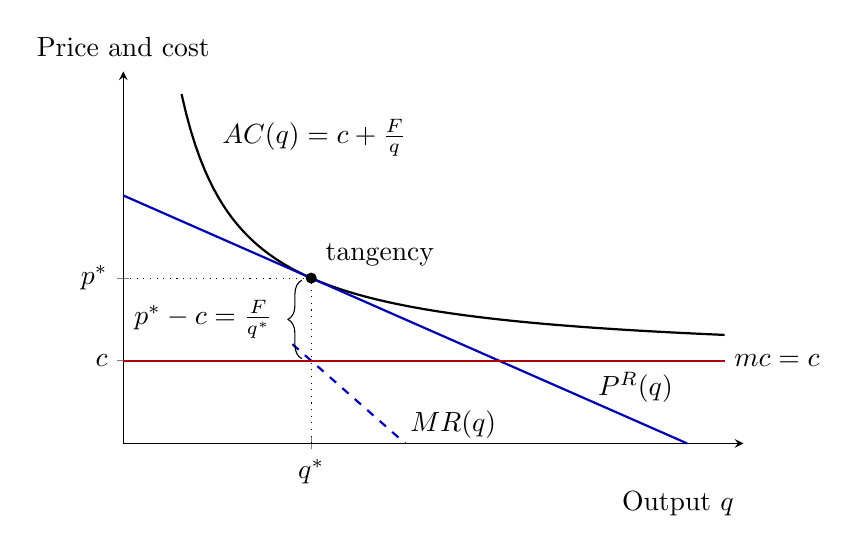
\begin{tikzpicture}
\begin{axis}[
  width=0.78\textwidth, height=0.52\textwidth,
  axis lines=left,
  xmin=0, xmax=6.6, ymin=0, ymax=9,
  xlabel={Output $q$}, ylabel={Price and cost},
  xtick={2}, xticklabels={$q^*$},
  ytick={2,4}, yticklabels={$c$,$p^*$},
  every axis x label/.style={at={(current axis.right of origin)}, anchor=north east, yshift=-14pt},
  every axis y label/.style={at={(current axis.above origin)}, anchor=south, yshift=2pt},
  clip=false]
  \addplot[thick, black, domain=0.62:6.4, samples=120] {2+4/x};
  \addplot[thick, blue!70!black, domain=0:6] {6-x};
  \addplot[thick, dashed, blue!70!black, domain=1.8:3] {6-2*x};
  \addplot[thick, red!70!black, domain=0:6.4] {2};
  \draw[dotted] (axis cs:2,0) -- (axis cs:2,4);
  \draw[dotted] (axis cs:0,4) -- (axis cs:2,4);
  \fill (axis cs:2,4) circle (2pt);
  \draw[decorate, decoration={brace, amplitude=5pt}] (axis cs:1.9,2.05) -- (axis cs:1.9,3.95)
    node[midway, left=7pt] {$p^* - c = \frac{F}{q^*}$};
  \node[anchor=west] at (axis cs:0.95,7.4) {$AC(q) = c + \frac{F}{q}$};
  \node[anchor=west] at (axis cs:4.95,1.35) {$P^R(q)$};
  \node[anchor=west] at (axis cs:2.95,0.45) {$MR(q)$};
  \node[anchor=west] at (axis cs:6.4,2) {$mc = c$};
  \node[anchor=south west] at (axis cs:2.05,4.05) {tangency};
\end{axis}
\end{tikzpicture}
\caption{The Chamberlin tangency under monopolistic competition. Free entry shifts the firm's inverse residual
demand $P^R(q)$ inward until it is tangent to average cost $AC(q) = c + \frac{F}{q}$ at $q^*$. There, marginal
revenue $MR(q)$ equals marginal cost $c$, and price equals average cost, so profit is zero. The markup
$p^* - c = \frac{F}{q^*}$ exactly covers the fixed cost. The curves are drawn for $c = 2$, $F = 4$ and
$P^R(q) = 6 - q$, which give $q^* = 2$ and $p^* = 4$.}
\label{fig:01-tangency}
\end{figure}

\citet[p.~1050]{Bresnahan1989} draws the welfare lesson. ``In the Chamberlinian tangency of monopolistic
competition, every firm has market power in the sense of this section. Yet that does not establish that there is
any inefficiency, once the need to cover the fixed costs of product design are taken into account.'' Forcing
every price down to marginal cost would leave each firm with a loss equal to its fixed cost, and some products
would disappear. Whether the market supplies too many or too few products depends on how much a product adds to
consumer surplus relative to the business it takes from rivals. Free entry can give too little variety under
monopolistic competition and too much entry in homogeneous-product markets \citep[see][and the work they
cite]{MankiwWhinston1986}. Bresnahan concludes that the welfare meaning of short-run market power with
differentiated products depends on the supply of new firms and new products. That supply is an empirical
question.

The same logic sits at the center of the recent debate over rising markups.
\citet{DeLoeckerEeckhoutUnger2020} estimate that the average ratio of price to marginal cost among US public
firms has risen since 1980. By \cref{prop:01-zero-profit-markup}, a higher markup need not mean higher profit if
fixed and overhead costs have risen as well. \Cref{sec:01-rising-markups} returns to this debate.

\subsection{The Cournot benchmark: concentration and margins}\label{sec:01-cournot-hhi}

We now have a measure of structure and a measure of market power. The simplest model that links them is the
Cournot model of quantity competition with a homogeneous good. Its central result motivates the cross-industry
regressions of \cref{sec:01-scp}. A small extension of the same result shows why those regressions are hard to
interpret.

\begin{assumption}[Homogeneous-good Cournot oligopoly]\label{ass:01-cournot}
\leavevmode
\begin{enumerate}[label=(\roman*)]
  \item There are $N$ firms selling a homogeneous good. Inverse market demand $P(Q)$ is twice differentiable,
  with $P'(Q) < 0$, where $Q = \sum_{i=1}^{N} q_i$.
  \item Firm $i$ has constant marginal cost $c_i$. It may also have a fixed cost, which does not affect its
  choice of output once it is active.
  \item Firms choose quantities simultaneously. Firm $i$ maximizes $\pi_i = \left(P(Q) - c_i\right) q_i$,
  taking its rivals' quantities as given.
  \item The equilibrium is interior. Every firm produces $q_i > 0$, and every firm's second-order condition
  $2P'(Q) + q_i P''(Q) < 0$ holds.
\end{enumerate}
\end{assumption}

\Cref{ch:theory} gives conditions for the existence and uniqueness of this equilibrium, and
\citet[Section~5.7.1]{Tirole1988} surveys them. Under mild boundary conditions, a pure-strategy equilibrium exists
when each firm's profit is concave in its own output, for which convex costs and concave demand suffice. With
two firms it is unique when the reaction functions have slopes below one in absolute value. Linear demand with
constant marginal cost gives the slope $-\frac{1}{2}$. Here we take an interior equilibrium as given. As in \cref{rem:01-residual}, the
market elasticity at the equilibrium is $\varepsilon = -\frac{P(Q)}{Q P'(Q)}$. Firm $i$'s Lerner index is
$L_i = \frac{P - c_i}{P}$, and the share-weighted average $\sum_i s_i L_i$ is the industry Lerner index.

\begin{proposition}[Cowling and Waterson]\label{prop:01-cowling-waterson}
Under \cref{ass:01-cournot}, every firm's Lerner index equals its market share divided by the market elasticity,
and the share-weighted Lerner index equals the Herfindahl-Hirschman index divided by the market elasticity:
\begin{equation}\label{eq:01-cowling-waterson}
  L_i = \frac{P - c_i}{P} = \frac{s_i}{\varepsilon}, \qquad \sum_{i=1}^{N} s_i L_i = \frac{\HHI}{\varepsilon} .
\end{equation}
\end{proposition}

\begin{proof}
Firm $i$'s first-order condition is
\[
  \frac{\partial \pi_i}{\partial q_i} = P(Q) + q_i P'(Q) - c_i = 0 .
\]
Rearrange it as $P - c_i = -q_i P'(Q)$ and divide by $P$:
\[
  \frac{P - c_i}{P} = -\frac{q_i P'(Q)}{P} .
\]
Multiply and divide the right side by $Q$:
\[
  \frac{P - c_i}{P} = \frac{q_i}{Q}\left(-\frac{Q P'(Q)}{P}\right) .
\]
The first factor is $s_i$ and the second is $\frac{1}{\varepsilon}$, which gives $L_i = \frac{s_i}{\varepsilon}$.
Multiply by $s_i$ and sum over firms:
\[
  \sum_{i=1}^{N} s_i L_i = \sum_{i=1}^{N} \frac{s_i^2}{\varepsilon} = \frac{\HHI}{\varepsilon} . \qedhere
\]
\end{proof}

The result is due to \citet{CowlingWaterson1976}. It fits together with the firm-level pricing rule. By
\eqref{eq:01-residual-elasticity}, firm $i$'s residual elasticity with rivals' output held fixed is
$\varepsilon^R_i = \frac{\varepsilon}{s_i}$, so
\[
  L_i = \frac{s_i}{\varepsilon} = \frac{1}{\varepsilon^R_i} .
\]
Each Cournot firm follows the inverse elasticity rule of \cref{prop:01-pricing-rule} for its own residual demand.
Large firms face less elastic residual demand and set higher margins. Since a firm's output and its margin are
chosen together, low-cost firms are both large and high-margin. \Cref{sec:01-demsetz} develops this observation
into the efficiency critique of regressions of profitability on concentration.

The same result links concentration to industry profit \citep[Section~5.5, eq.~5.14 and Exercise~5.6]{Tirole1988}.
Industry variable profit is
\[
  \Pi = \sum_{i=1}^{N} (P - c_i)\, q_i = \sum_{i=1}^{N} P L_i\, s_i Q = PQ \sum_{i=1}^{N} s_i L_i
  = \frac{PQ}{\varepsilon}\,\HHI .
\]
The second equality uses $P - c_i = P L_i$ and $q_i = s_i Q$, and the last uses \eqref{eq:01-cowling-waterson}.
The ratio of industry variable profit to industry revenue is therefore $\frac{\HHI}{\varepsilon}$. Suppose further
that demand has unit elasticity, $Q = \frac{k}{P}$ for a constant $k > 0$, so that consumers spend the fixed
amount $k$ on the good. Then $PQ = k$ and $\Pi = k\,\HHI$, which is Tirole's equation (5.15). In this case the
index measures industry profitability exactly, up to the constant $k$.

\begin{corollary}[Special cases]\label{cor:01-cournot-cases}
Under \cref{ass:01-cournot}, the following hold.
\begin{enumerate}[label=(\roman*)]
  \item With symmetric costs $c_i = c$, every firm has share $\frac{1}{N}$, $\HHI = \frac{1}{N}$, and
  $L = \frac{P - c}{P} = \frac{1}{N\varepsilon}$.
  \item With $N = 1$, $L = \frac{1}{\varepsilon}$, the monopoly inverse elasticity rule.
  \item With symmetric costs and an equilibrium elasticity bounded away from zero, $L \to 0$ and $P \to c$ as
  $N \to \infty$.
\end{enumerate}
\end{corollary}

\begin{proof}
With equal costs, the first-order conditions $P - c = -q_i P'(Q)$ have the same left side for every firm, so all
firms produce the same output and $s_i = \frac{1}{N}$. Then $\HHI = N \cdot \frac{1}{N^2} = \frac{1}{N}$, and all
the $L_i$ are equal to $L$, so \eqref{eq:01-cowling-waterson} gives (i). Setting $N = 1$ in (i) gives (ii). For
(iii), $L = \frac{1}{N\varepsilon}$ goes to zero when $\varepsilon$ stays above a positive constant, and
$L = 1 - \frac{c}{P} \to 0$ means $P \to c$.
\end{proof}

Statement (iii) is the sense in which Cournot competition approaches perfect competition as the number of firms
grows. The Cournot model therefore generates the hypothesis behind a generation of empirical work, namely that
margins rise with concentration. Read literally, \eqref{eq:01-cowling-waterson} suggests regressing the average
margin of each industry on its $\HHI$ across industries, with slope $\frac{1}{\varepsilon}$.

The Cournot result fixes the form of competition. To see what happens when conduct varies, we use a device from
the older literature. Suppose firm $i$ chooses its output as if its rivals' total output $Q_{-i} = Q - q_i$
responded to its own output at the rate
\[
  r_i = \frac{\dd Q_{-i}}{\dd q_i} .
\]
The number $r_i$ is firm $i$'s \emph{conjectural variation}. The firm then perceives
$\frac{\dd Q}{\dd q_i} = 1 + r_i$. Cournot behavior is $r_i = 0$.

\begin{proposition}[Margins and concentration under general conduct]\label{prop:01-clarke-davies}
Keep \cref{ass:01-cournot}, except that firm $i$ maximizes profit under the conjectural variation $r_i$, with
$1 + r_i \ge 0$. Then
\begin{equation}\label{eq:01-cv-lerner}
  L_i = \frac{s_i (1 + r_i)}{\varepsilon}, \qquad
  \sum_{i=1}^{N} s_i L_i = \frac{\theta}{\varepsilon}, \qquad
  \theta = \sum_{i=1}^{N} s_i^2 (1 + r_i) .
\end{equation}
Suppose conjectures are proportional, as in \citet{ClarkeDavies1982}. Firm $i$ expects every rival $j \ne i$ to
change its output by $\kappa$ times firm $i$'s own percentage change, for some $\kappa \in [0, 1]$. Then
\begin{equation}\label{eq:01-clarke-davies}
  r_i = \kappa\,\frac{1 - s_i}{s_i}, \qquad
  L_i = \frac{\kappa + (1 - \kappa)s_i}{\varepsilon}, \qquad
  \sum_{i=1}^{N} s_i L_i = \frac{\kappa + (1 - \kappa)\HHI}{\varepsilon} .
\end{equation}
\end{proposition}

\begin{proof}
Under the conjecture, firm $i$ perceives $\frac{\dd Q}{\dd q_i} = 1 + r_i$, so its perceived marginal profit is
\[
  \frac{\dd \pi_i}{\dd q_i} = P(Q) + q_i P'(Q) \frac{\dd Q}{\dd q_i} - c_i = P(Q) + q_i P'(Q)(1 + r_i) - c_i .
\]
Setting it to zero and following the steps in the proof of \cref{prop:01-cowling-waterson},
\begin{align}
  P + P'(Q)\, q_i (1 + r_i) &= c_i, \label{eq:01-cv-foc}\\
  \frac{P - c_i}{P} &= \frac{q_i}{Q}\left(-\frac{Q P'(Q)}{P}\right)(1 + r_i), \notag\\
  L_i &= \frac{s_i (1 + r_i)}{\varepsilon} . \notag
\end{align}
Multiplying by $s_i$ and summing gives
$\sum_i s_i L_i = \frac{1}{\varepsilon}\sum_i s_i^2 (1 + r_i) = \frac{\theta}{\varepsilon}$.

In the proportional case, the conjecture is $\frac{\dd q_j}{q_j} = \kappa\,\frac{\dd q_i}{q_i}$ for every
$j \ne i$, that is, $\frac{\dd q_j}{\dd q_i} = \kappa\,\frac{q_j}{q_i}$. Summing over rivals,
\[
  r_i = \sum_{j \ne i} \frac{\dd q_j}{\dd q_i} = \kappa\,\frac{Q_{-i}}{q_i} = \kappa\,\frac{Q - q_i}{q_i}
  = \kappa\,\frac{1 - s_i}{s_i} .
\]
Then
\[
  s_i (1 + r_i) = s_i + \kappa (1 - s_i) = \kappa + (1 - \kappa) s_i ,
\]
which gives the firm-level formula. Multiplying by $s_i$ and summing over firms,
\begin{align*}
  \theta = \sum_{i=1}^{N} s_i^2 (1 + r_i) &= \sum_{i=1}^{N} \left(\kappa s_i + (1 - \kappa) s_i^2\right) \\
  &= \kappa \sum_{i=1}^{N} s_i + (1 - \kappa) \sum_{i=1}^{N} s_i^2 \\
  &= \kappa + (1 - \kappa)\HHI ,
\end{align*}
where the last line uses $\sum_i s_i = 1$.
\end{proof}

The parameter $\theta$ is the index of industry conduct that we use throughout the book. Price-taking behavior,
$r_i = -1$ for every firm, gives $\theta = 0$ and $L_i = 0$. Cournot behavior, $r_i = 0$, gives
$\theta = \HHI$, which equals $\frac{1}{N}$ when firms are symmetric. In the Clarke-Davies family, $\kappa = 0$
is Cournot behavior and $\kappa = 1$ is joint profit maximization. With $\kappa = 1$ the firm expects all rivals
to move in proportion, so $1 + r_i = \frac{1}{s_i}$ and $q_i(1 + r_i) = Q$. Condition \eqref{eq:01-cv-foc} then
becomes $P + Q P'(Q) = c_i$, the first-order condition of a monopolist. With constant marginal costs, these
conditions can hold for all active firms only if their costs are equal, and the split of output among them is then
indeterminate. Every firm has $L_i = \frac{1}{\varepsilon}$ and $\theta = 1$. With rising marginal costs, as in
\cref{prop:01-supply-relation}, the same conditions equalize marginal costs across firms, as joint profit
maximization requires. Summing \eqref{eq:01-cv-foc} with weights $s_i$ gives the industry relation
\begin{equation}\label{eq:01-industry-relation}
  P = \bar c - \theta\, Q P'(Q), \qquad \bar c = \sum_{i=1}^{N} s_i c_i ,
\end{equation}
because $\sum_i s_i q_i (1 + r_i) = Q\sum_i s_i^2(1 + r_i) = Q\theta$. \Cref{sec:01-conduct-parameter} calls
\eqref{eq:01-industry-relation} the supply relation and shows how the New Empirical Industrial Organization is
built around it.

Conjectural variations must be read with care. In a static game a firm moves once and never observes a response,
so a ``conjecture'' about its rivals' reactions has no behavioral content within the game. The parameter
$\theta$ is best read as an index of how close the outcome is to the collusive one. \citet{Bresnahan1989}
stresses this reading, and \cref{sec:01-conduct-parameter} explains it. \Cref{ch:theory} discusses the theory of
conjectural variations and the conduct parameter.

\Cref{prop:01-clarke-davies} contains the main message of this section. In the Clarke-Davies family the average
margin is a linear function of the index,
\begin{equation}\label{eq:01-cd-line}
  \sum_{i=1}^{N} s_i L_i = \frac{\kappa}{\varepsilon} + \frac{1 - \kappa}{\varepsilon}\,\HHI ,
\end{equation}
with intercept $\frac{\kappa}{\varepsilon}$ and slope $\frac{1 - \kappa}{\varepsilon}$. Both depend on conduct and
on the demand elasticity. The slope is largest under Cournot behavior. It is zero under collusion, where margins
are at the monopoly level whatever the concentration. Panel (a) of \cref{fig:01-lerner-hhi} plots
\eqref{eq:01-cd-line} for $\varepsilon = 2$. The slope of margins on concentration is therefore no constant of
nature shared by all industries. This is at once the theoretical case for regressing margins on concentration
and the first reason such regressions fail. Industries differ in their elasticities and their conduct, and these
differences are correlated with concentration in ways that \cref{sec:01-scp-econometrics} explores.

Even within one industry with fixed conduct, the relation need not be linear, because the elasticity changes
with concentration. Take linear inverse demand $P(Q) = a - bQ$ with $a > c > 0$ and $b > 0$, and $N$ symmetric
Cournot firms with marginal cost $c$. The first-order condition $a - bQ - bq_i - c = 0$ holds for every firm, so
outputs are equal and $q_i = \frac{Q}{N}$. Summing the conditions over firms and solving,
\begin{align*}
  N(a - c) - NbQ - bQ &= 0, \\
  Q &= \frac{N(a - c)}{b(N + 1)}, \\
  P = a - bQ &= \frac{a + Nc}{N + 1} .
\end{align*}
The Lerner index and the market elasticity at the equilibrium are
\begin{align*}
  L &= \frac{P - c}{P} = \frac{\frac{a - c}{N + 1}}{\frac{a + Nc}{N + 1}} = \frac{a - c}{a + Nc}, \\
  \varepsilon &= \frac{P}{bQ} = \frac{a + Nc}{N(a - c)} .
\end{align*}
Substitute $N = \frac{1}{\HHI}$ and multiply each numerator and denominator by $\HHI$:
\begin{equation}\label{eq:01-linear-cournot-LH}
  L = \frac{(a - c)\HHI}{a\HHI + c}, \qquad \varepsilon = \frac{a\HHI + c}{a - c} .
\end{equation}
As a check, $\frac{\HHI}{\varepsilon} = \frac{(a - c)\HHI}{a\HHI + c} = L$, as \cref{prop:01-cowling-waterson}
requires. The elasticity rises with concentration, because fewer firms means a higher price and a lower quantity
along a linear demand curve. Differentiating $L$ with respect to $\HHI$,
\begin{align*}
  \frac{\dd L}{\dd \HHI} &= \frac{(a - c)(a\HHI + c) - (a - c)\HHI \cdot a}{(a\HHI + c)^2}
  = \frac{c(a - c)}{(a\HHI + c)^2} > 0, \\
  \frac{\dd^2 L}{\dd \HHI^2} &= -\frac{2ac(a - c)}{(a\HHI + c)^3} < 0 .
\end{align*}
The margin rises with concentration at a decreasing rate. Panel (b) of \cref{fig:01-lerner-hhi} plots the curve
for two values of the ratio $\frac{c}{a}$. A higher ratio of marginal cost to the demand intercept lowers the
whole curve. Industries with different cost-demand ratios lie on different curves, so even the causal effect of
concentration on margins differs across industries. Throughout this calculation $N$ is fixed. When entry
determines $N$, concentration becomes an equilibrium outcome itself, a problem that \cref{sec:01-endogeneity}
takes up.

\begin{figure}[htbp]
\centering
\begin{subfigure}[t]{0.49\textwidth}
\centering
\begin{tikzpicture}[baseline=(current axis.north)]
\begin{axis}[
  scale only axis, width=0.78\linewidth, height=0.66\linewidth,
  xmin=0, xmax=1, ymin=0, ymax=0.6,
  xlabel={$\HHI$}, ylabel={$\sum_i s_i L_i$},
  xtick={0,0.25,0.5,0.75,1}, ytick={0,0.1,0.2,0.3,0.4,0.5,0.6},
  tick label style={font=\footnotesize}, label style={font=\small},
  domain=0:1, samples=2,
  legend columns=2,
  legend style={font=\footnotesize, at={(0.5,-0.24)}, anchor=north, draw=none, column sep=4pt},
  legend cell align=left]
  \addplot[thick, black] {x/2};
  \addlegendentry{$\kappa = 0$ (Cournot)}
  \addplot[thick, blue!70!black, dashed] {(0.25+0.75*x)/2};
  \addlegendentry{$\kappa = 0.25$}
  \addplot[thick, red!70!black, densely dotted] {(0.5+0.5*x)/2};
  \addlegendentry{$\kappa = 0.5$}
  \addplot[thick, green!45!black, dashdotted] {0.5};
  \addlegendentry{$\kappa = 1$ (collusion)}
\end{axis}
\end{tikzpicture}
\caption{Clarke-Davies conduct, $\varepsilon = 2$}
\end{subfigure}\hfill
\begin{subfigure}[t]{0.49\textwidth}
\centering
\begin{tikzpicture}[baseline=(current axis.north)]
\begin{axis}[
  scale only axis, width=0.78\linewidth, height=0.66\linewidth,
  xmin=0, xmax=1, ymin=0, ymax=0.75,
  xlabel={$\HHI$}, ylabel={$L$},
  xtick={0,0.25,0.5,0.75,1}, ytick={0,0.1,0.2,0.3,0.4,0.5,0.6,0.7},
  tick label style={font=\footnotesize}, label style={font=\small},
  domain=0:1, samples=101,
  legend columns=2,
  legend style={font=\footnotesize, at={(0.5,-0.24)}, anchor=north, draw=none, column sep=4pt},
  legend cell align=left]
  \addplot[thick, black] {8*x/(10*x+2)};
  \addlegendentry{$\frac{c}{a} = 0.2$}
  \addplot[thick, blue!70!black, dashed] {5*x/(10*x+5)};
  \addlegendentry{$\frac{c}{a} = 0.5$}
  \addplot[only marks, mark=*, mark size=1.3pt, black,
    samples at={1,0.5,0.333333,0.25,0.2,0.166667,0.142857,0.125,0.111111,0.1}]
    {8*x/(10*x+2)};
  \addlegendentry{$\HHI = \frac{1}{N}$}
  \addplot[only marks, mark=*, mark size=1.3pt, blue!70!black,
    samples at={1,0.5,0.333333,0.25,0.2,0.166667,0.142857,0.125,0.111111,0.1}, forget plot]
    {5*x/(10*x+5)};
\end{axis}
\end{tikzpicture}
\caption{Symmetric Cournot, linear demand}
\end{subfigure}
\caption{Margins and concentration. Panel (a) plots the share-weighted Lerner index against the
Herfindahl-Hirschman index in the Clarke-Davies family,
$\sum_i s_i L_i = \frac{\kappa + (1 - \kappa)\HHI}{\varepsilon}$, for $\varepsilon = 2$. The lines run from
$\left(0, \frac{\kappa}{\varepsilon}\right)$ to $\left(1, \frac{1}{\varepsilon}\right)$. Panel (b) plots the
symmetric Cournot relation with linear demand, $L = \frac{(a - c)\HHI}{a\HHI + c}$, for $\frac{c}{a} = 0.2$ and
$\frac{c}{a} = 0.5$. Dots mark $\HHI = \frac{1}{N}$ for $N = 1, \dots, 10$.}
\label{fig:01-lerner-hhi}
\end{figure}

\section{The structure-conduct-performance paradigm}\label{sec:01-scp}

For about three decades the main empirical program in industrial organization put one question to
cross-industry data. Do more concentrated industries earn higher margins? The program is known as the
\emph{structure-conduct-performance} (SCP) paradigm. This section states its logic, formalizes the
experiment it had in mind, and describes how it was carried out. \Cref{sec:01-scp-econometrics} then asks
what its regressions identify, and \cref{sec:01-scp-after} follows the debates it left behind.

\subsection{The SCP mechanism}\label{sec:01-scp-mechanism}

The paradigm describes a causal chain with four links, summarized in \cref{fig:01-scp-flow}. \emph{Basic
conditions} are the primitives of an industry. On the supply side they include technology, unionization,
the transportability of the product and the legal environment. On the demand side they include
preferences, the growth of demand and its seasonality. Basic conditions determine \emph{market
structure}, which comprises the number of sellers and buyers, the extent of vertical integration, and the
degree of vertical and horizontal product differentiation. Structure determines conduct, the
pricing, advertising and investment decisions of firms. Conduct in turn determines \emph{performance},
measured by profits and by welfare.

\citet[Introduction]{Tirole1988} calls this program the ``Harvard tradition'' and associates it with Joe Bain
and Edward Mason. In his history it was the first of two waves of interest in industrial organization, and it
was empirical in nature. His statement of the chain is close to ours. Structure comprises the number of sellers,
their degree of product differentiation, the cost structure and the degree of vertical integration with
suppliers. Conduct comprises price, research and development, investment and advertising. Performance comprises
efficiency, the ratio of price to marginal cost, product variety, the rate of innovation, profits and
distribution. Tirole adds that the paradigm, although plausible, often rested on loose theories.

\begin{figure}[htbp]
\centering
\begin{tikzpicture}[
  box/.style={draw, rounded corners=2pt, align=flush left, text width=3.15cm,
    inner sep=4pt, font=\footnotesize},
  fwd/.style={-{Stealth[length=2.2mm]}, thick},
  back/.style={-{Stealth[length=2mm]}, dashed, gray!65!black},
  lab/.style={font=\scriptsize, align=center, text=gray!25!black}]
\node[box] (bc) {\parbox[t][2.85cm][t]{\linewidth}{\raggedright\textbf{Basic conditions}\\[3pt]
  Supply: technology, unions, transportability, legal environment.\\[3pt]
  Demand: preferences, growth, seasonality.}};
\node[box, right=0.62cm of bc] (ms) {\parbox[t][2.85cm][t]{\linewidth}{\raggedright\textbf{Market structure}\\[3pt]
  Number of sellers and buyers, vertical integration, vertical and horizontal product
  differentiation.}};
\node[box, right=0.62cm of ms] (cd) {\parbox[t][2.85cm][t]{\linewidth}{\raggedright\textbf{Conduct}\\[3pt]
  Pricing, advertising, investment.}};
\node[box, right=0.62cm of cd] (pf) {\parbox[t][2.85cm][t]{\linewidth}{\raggedright\textbf{Performance}\\[3pt]
  Profits, welfare.}};
\draw[fwd] (bc) -- (ms);
\draw[fwd] (ms) -- (cd);
\draw[fwd] (cd) -- (pf);
\draw[back] (cd.-115) to[out=-120, in=-60] node[lab, below=1pt] {mergers, advertising,\\ R\&D}
  (ms.-65);
\draw[back] (pf.-100) to[out=-115, in=-65, looseness=0.85]
  node[lab, below=1pt] {entry and exit respond to profits} (ms.-115);
\draw[back] (cd.110) to[out=125, in=55, looseness=0.8]
  node[lab, above=1pt] {R\&D changes technology, lobbying changes the legal environment}
  (bc.70);
\end{tikzpicture}
\caption{The structure-conduct-performance paradigm. Solid arrows show the causal chain that the
paradigm assumes. Dashed arrows show feedback that it ignores. Conduct and performance shape market
structure, and conduct reshapes basic conditions. Once the dashed arrows are admitted, market structure
is an equilibrium outcome.}
\label{fig:01-scp-flow}
\end{figure}

The chain has a strong implication for policy. If structure causes performance, a regulator can improve
performance by acting on structure, for example by blocking mergers or breaking up dominant firms. The
empirical task then reduces to measuring how performance varies with structure. Conduct rarely needs to
be observed, because structure is assumed to pin it down.

The dashed arrows in \cref{fig:01-scp-flow} show why the chain is incomplete. Profits attract entry and
losses induce exit, so performance feeds back into the number of sellers. Mergers, advertising and
research and development (R\&D) are forms of conduct, yet they shape concentration and differentiation.
Research changes technology and lobbying changes the legal environment, so conduct also feeds back into
basic conditions. In modern terms, market structure is an equilibrium outcome, determined jointly with
conduct and performance by the basic conditions. \Cref{sec:01-scp-econometrics} works out the
consequences of this observation for the regressions that the paradigm relied on.

The ideal experiment behind the paradigm is easy to state. We would take many otherwise identical
industries, randomly assign each one a market structure, and compare their performance. In practice,
researchers compared markups or profitability across existing industries with different levels of
concentration. The gap between the two designs can be stated precisely in the language of potential
outcomes, which \cref{app:econometrics} reviews.

\begin{definition}[Potential margins]\label{def:01-potential-margins}
Index industries by $k = 1, \dots, n$. For each concentration level $h \in (0, 1]$, let $L_k(h)$ be the
industry-wide Lerner index that industry $k$ would have if an outside intervention set its Herfindahl
index to $h$. The intervention holds the demand, costs and conduct of the industry fixed. The function
$h \mapsto L_k(h)$ is the \emph{causal curve} of industry $k$. We observe only the realized margin $L_k
= L_k(\HHI_k)$.
\end{definition}

The industry-wide Lerner index is the share-weighted index $\sum_i s_i L_i$ of
\cref{prop:01-cowling-waterson}. An intervention that sets $h$ could be a regulator that fixes the number
of licenses in an industry of symmetric firms. Now compare the average margins of industries observed at
two concentration levels $h$ and $h'$. We add and subtract $\E[L_k(h') \mid \HHI_k = h]$:
\begin{align}
\E[L_k \mid \HHI_k = h] - \E[L_k \mid \HHI_k = h']
  &= \E[L_k(h) \mid \HHI_k = h] - \E[L_k(h') \mid \HHI_k = h'] \notag \\
  &= \underbrace{\E[L_k(h) - L_k(h') \mid \HHI_k = h]}_{\text{causal effect at } h} \notag \\
  &\quad + \underbrace{\E[L_k(h') \mid \HHI_k = h] - \E[L_k(h') \mid \HHI_k = h']}_{\text{selection}}.
  \label{eq:01-potential-outcomes}
\end{align}
The first equality uses $L_k = L_k(\HHI_k)$. The first term after the second equality is the average
causal effect of moving from $h'$ to $h$ among the industries observed at $h$. The second term compares
the margins that
two different groups of industries would earn at the same concentration $h'$. It differs from zero
whenever the industries that end up concentrated differ in demand, cost or conduct from those that do
not. Random assignment makes $\HHI_k$ independent of the whole curve $L_k(\cdot)$. The selection term
then vanishes, and the first term becomes the population average effect $\E[L_k(h) - L_k(h')]$.

\begin{example}[Selection on the demand elasticity]\label{ex:01-selection-elasticity}
Suppose industry $k$ has constant-elasticity demand with elasticity $\varepsilon_k$ and symmetric
Cournot firms. By \cref{prop:01-cowling-waterson}, its causal curve is
$L_k(h) = \frac{h}{\varepsilon_k}$. Substituting into \eqref{eq:01-potential-outcomes}, the selection
term equals
\[
h' \left( \E\left[\frac{1}{\varepsilon_k} \,\middle|\, \HHI_k = h\right]
        - \E\left[\frac{1}{\varepsilon_k} \,\middle|\, \HHI_k = h'\right] \right).
\]
Its sign depends on how industries sort. Margins are higher where demand is less elastic, so free entry
tends to draw more firms into those industries and to make them less concentrated. The conditional mean
of $\frac{1}{\varepsilon_k}$ then falls with concentration, and the selection term is negative for
$h > h'$. If inelastic demand instead goes with high fixed costs, the term can be positive.
\end{example}

\subsection{Origins and practice}\label{sec:01-scp-practice}

The SCP approach grew out of the Harvard tradition associated with \citet{Mason1939}. As its title indicates,
Mason's article studied the price and production policies of large-scale enterprise.
Joe Bain turned the SCP view into a statistical program. \citet{Bain1951} related
the profit rates of American manufacturing industries over 1936--1940 to their concentration.
\citet{Bain1951,Bain1956} hypothesized that concentration facilitates collusion between firms and so raises
industry-wide profits \citep[Section~5.5]{Tirole1988}. \citet[p.~46]{LevensteinSuslow2006} attribute the same
hypothesis to Bain. \citet{Bain1956} added the theory of \emph{barriers to entry}, the advantages of established
sellers over potential entrants. In Tirole's paraphrase, a barrier to entry is anything that lets incumbent firms
earn supranormal profits without the threat of entry \citep[Chapter~8, introduction]{Tirole1988}. Tirole lists
the four elements of market structure that Bain identified informally. They are economies of scale, absolute cost
advantages, product-differentiation advantages and capital requirements, the last of which Tirole calls
controversial. Bain also distinguished three cases. Entry is blockaded when incumbents ignore the threat and entry
is still unattractive. It is deterred when incumbents change their behavior to prevent it, and accommodated when
they find it more profitable to let entrants in. For the quarter century that followed \citet{Bain1951}, the
cross-section study of many industries was the main empirical method of the field \citep[p.~1012]{Bresnahan1989}.
\citet{Schmalensee1989} wrote its definitive review.

A typical study used one cross-section of industries. The dependent variable was an accounting measure
of profitability, such as the profit rate on equity or assets or the price-cost margin computed from the
Census of Manufactures. The key regressor was a concentration measure, often the four-firm ratio
$\mathit{CR}_4$ or the Herfindahl index of \cref{def:01-concentration}. The canonical specification is
\begin{equation}\label{eq:01-scp-regression}
\pi_k = \beta_0 + \beta_1 \HHI_k + \varphi^\top X_k + e_k, \qquad k = 1, \dots, n,
\end{equation}
where $\pi_k$ is the profitability measure of industry $k$ and $e_k$ is an error term. The Herfindahl
index may be replaced by $\mathit{CR}_{4,k}$. The vector $X_k$ collects controls, typically the ratios of
R\&D spending, capital and advertising spending to sales, together with the import share. Its
coefficients are $\varphi$, and the whole equation is estimated by ordinary least squares (OLS). The typical finding was
$\hat\beta_1 > 0$. It was read as evidence that concentration raises margins, and hence that
concentration is harmful.

\citet[Introduction]{Tirole1988} writes the typical regression as $\pi_k = f(\mathit{CR}_k, \mathit{BE}_k, \dots)$,
run on a cross-section of many industries. Here $\mathit{CR}_k$ is a concentration ratio and $\mathit{BE}_k$
collects measures of barriers to entry. Two common measures were the ratio of advertising to sales and the
\emph{minimum efficient scale} of entry, the smallest output at which average cost reaches its minimum.
Regression \eqref{eq:01-scp-regression} is the linear version. Tirole stresses that its coefficients are
correlations, or ``descriptive statistics,'' and not causal relationships. Industry profit, the concentration
ratio and the ratio of advertising to sales ``are jointly endogenous.'' The basic conditions of the market and
the behavior of its firms determine all three at once.

The tradition also tried to measure basic conditions directly, scale economies in particular
\citep[Introduction, note~4]{Tirole1988}. The most common method estimates a cost function of output and input
prices. Bain built ``engineering production functions'' from engineering data on plants, and he asked managers
what the optimal plant size was. George Stigler's \emph{survivorship technique} infers efficient scale instead
from the sizes of the firms that survive. Tirole notes that such measures are hard to make accurate and
comparable across industries.

The design reflected the econometric practice of its time. Samples were small, the data were industry
aggregates, and matrices were sometimes inverted by hand. Identification in the modern sense received
little attention. Concentration was treated as an exogenous regressor, and its coefficient was read as a
structural constant.

\citet[p.~146]{EinavLevin2010} describe two challenges that held the field back into the 1970s. The
first was the lack of compelling theoretical models of imperfect competition, which the game theory
revolution of the 1980s later supplied. The second was the lack of good data and of convincing
strategies for testing hypotheses about competition. Researchers knew that concentration might depend on
the same factors as profitability. More sophisticated studies tried to fix this by treating concentration
as driven by ``exogenous'' barriers to entry, such as scale economies, advertising or R\&D
\citep[p.~146]{EinavLevin2010}. Yet advertising intensity and capital intensity are chosen by firms, so
they are hard to defend as instruments \citep[p.~147]{EinavLevin2010}. \citet[p.~954]{Schmalensee1989}
opened his review by acknowledging that ``essentially all variables that have been employed in such
studies are logically endogenous'' (quoted in \citealp[p.~147]{EinavLevin2010}).

\citet[Introduction, note~2]{Tirole1988} recommends the review of \citet{Schmalensee1989}, which he dates 1986,
as an excellent survey and assessment of this approach. His own summary of the evidence records two facts that frame the rest
of this chapter (note~3). First, the cross-industry relation between rates of return and concentration ``is weak.'' Second,
``introducing a market-share variable on the right-hand side of the regression tends to wipe out
concentration-ratio effects.'' Tirole explains the second fact by cost heterogeneity. In industries where a few
low-cost firms produce most of the output, concentration and profits are both high. The concentration ratio may
then pick up the effect of the omitted market share. The first fact motivates \cref{sec:01-scp-econometrics},
and the second lies at the center of the Demsetz debate in \cref{sec:01-demsetz}. \Cref{sec:01-neio-principles} returns to the maintained
hypotheses of the paradigm that the next generation of research rejected.

\section{What cross-industry regressions identify}\label{sec:01-scp-econometrics}

Regression \eqref{eq:01-scp-regression} always estimates something. Its probability limit is a
linear projection coefficient, and the question is whether that coefficient measures an economic
object. This section takes the problems in turn. Margins are mismeasured (\cref{sec:01-accounting}),
concentration is mismeasured (\cref{sec:01-market-def-error}), and concentration is endogenous
(\cref{sec:01-endogeneity}). A Monte Carlo experiment shows the size of the problems
(\cref{sec:01-montecarlo}), and \cref{sec:01-salinger} asks whether panel data solve them.

\subsection{Measurement: accounting versus economic margins}\label{sec:01-accounting}

The theory of \cref{sec:01-cournot-hhi} concerns the Lerner index $L = \frac{p - mc}{p}$. SCP studies
used accounting data instead. The most common margin was the \emph{Census price-cost margin},
\begin{equation}\label{eq:01-pcm}
\mathit{PCM} = \frac{\text{value of shipments} - \text{payroll} - \text{cost of materials}}
                    {\text{value of shipments}},
\end{equation}
computed for each manufacturing industry from the Census of Manufactures. It nets out the main variable
inputs and ignores the cost of capital. The next proposition shows what it measures. In this subsection
only, $\rho$ denotes the rental price of capital (elsewhere in the book $\rho$ is the pass-through rate).

\begin{proposition}[What the Census margin measures]\label{prop:01-pcm-bias}
Consider an industry that sells output $q > 0$ at price $p$, so that sales are $S = pq$. Payroll and
materials form the variable cost $VC(q)$, with $VC(0) = 0$ and marginal cost $mc(q) = VC'(q)$. The
industry uses a capital stock $K$ with rental price $\rho$, the interest and depreciation cost per dollar
of capital. Economic profit is $\pi = pq - VC(q) - \rho K$.
\begin{enumerate}[label=(\roman*)]
\item If $VC(q) = cq$, then $\mathit{PCM} = \frac{p - c}{p} = L$.
\item In general, $\mathit{PCM} = \frac{\pi}{S} + \rho \frac{K}{S}$. An industry that earns zero economic
profit has $\mathit{PCM} = \rho \frac{K}{S} > 0$.
\item If $VC$ is convex, then $\mathit{PCM} \ge L$. The inequality is strict if $VC$ is strictly convex.
\end{enumerate}
\end{proposition}

\begin{proof}
By definition, $\mathit{PCM} = \frac{S - VC(q)}{S}$. For (i), substitute $VC(q) = cq$:
\[
\mathit{PCM} = \frac{pq - cq}{pq} = \frac{p - c}{p} = L.
\]
For (ii), the definition of economic profit gives $pq - VC(q) = \pi + \rho K$. Divide both sides by $S$:
\[
\mathit{PCM} = \frac{pq - VC(q)}{S} = \frac{\pi + \rho K}{S} = \frac{\pi}{S} + \rho \frac{K}{S}.
\]
Setting $\pi = 0$ gives $\mathit{PCM} = \rho \frac{K}{S}$, which is positive whenever $K > 0$. For (iii),
write $\mathit{PCM} = \frac{p - AVC(q)}{p}$ with average variable cost $AVC(q) = \frac{VC(q)}{q}$. A convex
function lies above its tangent lines, so
\[
VC(0) \ge VC(q) + VC'(q)(0 - q).
\]
With $VC(0) = 0$, this reads $q \, mc(q) \ge VC(q)$, so $AVC(q) \le mc(q)$. Therefore
\[
\mathit{PCM} = \frac{p - AVC(q)}{p} \ge \frac{p - mc(q)}{p} = L.
\]
Strict convexity makes the tangent inequality strict for $q > 0$.
\end{proof}

The Census margin therefore mixes three things: the Lerner index, the return to capital, and the
curvature of variable cost. Capital-intensive industries show high margins even when they earn no rents.
Capital intensity also tends to raise minimum efficient scale and hence concentration. A regression of
$\mathit{PCM}$ on concentration that omits capital intensity then attributes the return to capital to
concentration.

\begin{corollary}[Omitted capital intensity]\label{prop:01-pcm-ovb}
Suppose economic profitability satisfies $\frac{\pi_k}{S_k} = \beta_0 + \beta_1 \HHI_k + e_k$, where
$e_k$ is uncorrelated with $\HHI_k$ and with $\frac{K_k}{S_k}$, and the rental price $\rho$ is common to
all industries. Then OLS of $\mathit{PCM}_k$ on a constant and $\HHI_k$ converges to
\[
\beta_1 + \rho \, \frac{\Cov\left(\frac{K_k}{S_k}, \HHI_k\right)}{\Var(\HHI_k)}.
\]
\end{corollary}

\begin{proof}
By \cref{prop:01-pcm-bias}(ii), $\mathit{PCM}_k = \beta_0 + \beta_1 \HHI_k + \rho \frac{K_k}{S_k} + e_k$.
The OLS slope converges to $\frac{\Cov(\mathit{PCM}_k, \HHI_k)}{\Var(\HHI_k)}$. Substituting,
\[
\frac{\Cov(\mathit{PCM}_k, \HHI_k)}{\Var(\HHI_k)}
 = \beta_1 + \rho \frac{\Cov\left(\frac{K_k}{S_k}, \HHI_k\right)}{\Var(\HHI_k)}
   + \frac{\Cov(e_k, \HHI_k)}{\Var(\HHI_k)},
\]
and the last term is zero by assumption.
\end{proof}

This is why \citet{CollinsPreston1969} and most later studies included the capital-sales ratio
$\frac{K}{S}$ as a regressor next to concentration. The control removes the bias in
\cref{prop:01-pcm-ovb} only if $\rho$ is common across industries and capital is measured correctly.

Accounting rates of return on equity or assets have their own problems. \citet{FisherMcGowan1983} showed
that the accounting rate of return can differ widely from the economic rate of return, which is the
internal rate of return on an investment. The gap depends on the time profile of cash flows and on
depreciation rules, so it varies across industries even when no industry earns rents. Inflation and the
valuation of assets at historical cost add further distortions. A simple case shows the direction of
one common bias.

\begin{remark}[Expensed intangible capital]\label{rem:01-intangibles}
Consider a firm in a steady state with tangible capital $K$. It also builds an intangible stock $A$, such
as brand capital or knowledge, by spending $I$ per period on advertising or R\&D. The stock depreciates
at rate $d_A$, so in the steady state $A = \frac{I}{d_A}$. Let $R$ be revenue net of variable costs and
of the depreciation of tangible capital. Economic depreciation of the intangible stock is $d_A A = I$, so
the economic rate of return on all capital is
\[
r^e = \frac{R - d_A A}{K + A} = \frac{R - I}{K + A}.
\]
Accounting rules expense $I$ and leave $A$ off the balance sheet, so the accounting rate of return is
$r^{acc} = \frac{R - I}{K}$. Dividing the two expressions gives
\[
\frac{r^{acc}}{r^e} = \frac{K + A}{K} = 1 + \frac{A}{K} > 1.
\]
When $R > I$, accounting returns overstate economic returns, and they do so most in industries that are
intensive in advertising or R\&D. If those industries are also more concentrated, the measured profit-concentration relation is
biased upward.
\end{remark}

The controls that theory calls for are the demand elasticity, the height of entry barriers and the degree
of product differentiation. They are hard to measure, so SCP studies rarely included them. The
regression thus omits the very variables that theory says determine margins. \Cref{sec:01-cournot-hhi}
showed that the slope of margins on concentration is $\frac{1 - \kappa}{\varepsilon}$, which depends on
conduct and on the demand elasticity. \Cref{tab:01-scp-data} compares what theory needs with what the
studies measured.

\begin{table}[htbp]
\centering\footnotesize
\renewcommand{\arraystretch}{1.2}
\caption{What the theory of margins needs and what SCP studies measured}
\label{tab:01-scp-data}
\begin{tabularx}{\linewidth}{@{}>{\raggedright\arraybackslash}p{2.1cm}
  >{\raggedright\arraybackslash}X>{\raggedright\arraybackslash}X>{\raggedright\arraybackslash}X@{}}
\toprule
Object & What theory needs & What SCP studies used & Consequence for the regression \\
\midrule
Margin & Lerner index $\frac{p - mc}{p}$ & Accounting profit rate, return on assets, Census
  $\mathit{PCM}$ & Mixes rents with the return to capital and cost curvature
  (\cref{prop:01-pcm-bias}, \cref{rem:01-intangibles}) \\
Concentration & Shares in the economic market (\cref{sec:01-market-definition}) & National shares in a
  four-digit SIC industry & Measurement error and attenuation (\cref{sec:01-market-def-error}) \\
Demand elasticity & $\varepsilon$, which scales the slope & Rarely measured & Omitted variable that
  enters the slope itself \\
Entry barriers & Sunk and fixed costs, regulation & Capital, advertising and R\&D intensities &
  The proxies are chosen by firms, hence endogenous \\
Differentiation & Substitution patterns among products & Advertising intensity, at best & Crude and
  endogenous proxy \\
Conduct & $\kappa$ or $\theta$ (\cref{prop:01-clarke-davies}) & Not measured, implicitly common & The
  slope averages over conduct regimes (\cref{prop:01-scp-plim}) \\
Foreign competition & Imports in the relevant market & Import share & Partial correction of national
  shares \\
\bottomrule
\end{tabularx}
\end{table}

\subsection{Market definition and measurement error in concentration}\label{sec:01-market-def-error}

Concentration is defined relative to a market (\cref{sec:01-market-definition}). SCP studies used
industries as defined by the Standard Industrial Classification (SIC), usually at the four-digit level.
The SIC was replaced by the North American Industry Classification System (NAICS) in 1997. These
classifications group plants by production process more than by substitution in demand. A four-digit
industry can be too broad, pooling products that do not compete with each other. It can also be too
narrow, leaving out close substitutes classified elsewhere and leaving out imports. Census concentration
ratios are national, while many products are sold in local markets because transport is costly. Cement,
ready-mixed concrete and newspapers are standard examples. The next lemma shows how large the resulting
error can be.

\begin{lemma}[Pooling local markets]\label{prop:01-pooled-hhi}
Suppose a national industry consists of $G$ local markets of equal size. Each local market $\ell$ is
served by its own firms and has Herfindahl index $\HHI_\ell$. Then the national Herfindahl index is
\[
\HHI^{nat} = \frac{1}{G} \left( \frac{1}{G} \sum_{\ell = 1}^{G} \HHI_\ell \right).
\]
\end{lemma}

\begin{proof}
Let $s_{i\ell}$ be the share of firm $i$ in local market $\ell$. Because the markets have equal size, the
national share of that firm is $\frac{s_{i\ell}}{G}$. Summing squared national shares over all firms,
\[
\HHI^{nat} = \sum_{\ell = 1}^{G} \sum_{i} \left( \frac{s_{i\ell}}{G} \right)^2
 = \frac{1}{G^2} \sum_{\ell = 1}^{G} \sum_{i} s_{i\ell}^2
 = \frac{1}{G^2} \sum_{\ell = 1}^{G} \HHI_\ell .
\]
Rearranging the last expression gives the result.
\end{proof}

National concentration thus understates local concentration by the factor $G$. Two industries with the
same local Herfindahl index of $0.5$, one sold nationally and one sold in 50 separate local markets, have
national indices of $0.5$ and $0.01$. The number of local markets differs across industries with transport
costs, so this error is large, systematic and correlated with industry characteristics. It cannot be
treated as noise.

Even classical noise has a known cost. Suppose the true relation is $L_k = \beta_0 + \beta_1 \HHI^*_k +
e_k$, and we observe $\HHI_k = \HHI^*_k + u_k$. Assume $u_k$ has mean zero and variance $\sigma_u^2$ and
is uncorrelated with $\HHI^*_k$ and $e_k$. The OLS slope of $L_k$ on $\HHI_k$ converges to
\begin{equation}\label{eq:01-attenuation}
\frac{\Cov(\beta_0 + \beta_1 \HHI^*_k + e_k, \, \HHI^*_k + u_k)}{\Var(\HHI^*_k + u_k)}
 = \frac{\beta_1 \Var(\HHI^*_k)}{\Var(\HHI^*_k) + \sigma_u^2}
 \equiv \beta_1 \chi .
\end{equation}
The numerator keeps only $\beta_1 \Var(\HHI^*_k)$ because the other covariances are zero. The
\emph{reliability ratio} $\chi \in (0, 1]$ is the share of the variance of measured concentration that
is signal. Measurement error biases the slope toward zero, and \cref{sec:01-salinger} shows that panel
methods can make this bias much worse.

\subsection{Endogeneity of structure: theory}\label{sec:01-endogeneity}

Suppose margins and concentration were measured without error. OLS still converges to a projection
coefficient, and the next proposition characterizes it. The industry-level model is the
conduct-adjusted Cowling-Waterson relation of \cref{prop:01-clarke-davies}
\citep{CowlingWaterson1976,ClarkeDavies1982}.

\begin{proposition}[What the SCP slope converges to]\label{prop:01-scp-plim}
Let $(L_k, \HHI_k)$ be independent and identically distributed across industries with finite second
moments and $\Var(\HHI_k) > 0$.
\begin{enumerate}[label=(\roman*)]
\item The OLS slope of $L_k$ on a constant and $\HHI_k$ converges in probability to
$\frac{\Cov(L_k, \HHI_k)}{\Var(\HHI_k)}$.
\item Suppose every industry satisfies $L_k = A_k + B_k \HHI_k$ with $A_k = \frac{\kappa_k}{\varepsilon_k}$
and $B_k = \frac{1 - \kappa_k}{\varepsilon_k}$, where $\kappa_k$ is the Clarke-Davies conduct parameter and
$\varepsilon_k$ the market elasticity of industry $k$. Then the slope converges to
\begin{equation}\label{eq:01-scp-plim}
\E[B_k] + \frac{\Cov(A_k, \HHI_k) + \Cov(B_k, \HHI_k^2) - \E[\HHI_k] \Cov(B_k, \HHI_k)}{\Var(\HHI_k)}.
\end{equation}
\item If $(\kappa_k, \varepsilon_k)$ is independent of $\HHI_k$, the slope converges to
$\E\left[\frac{1 - \kappa_k}{\varepsilon_k}\right]$ and the intercept to
$\E\left[\frac{\kappa_k}{\varepsilon_k}\right]$.
\end{enumerate}
\end{proposition}

\begin{proof}
(i) The OLS slope is the ratio of the sample covariance of $(L_k, \HHI_k)$ to the sample variance of
$\HHI_k$. By the law of large numbers each converges to its population counterpart, and the continuous
mapping theorem gives the limit of the ratio. (ii) Write $H = \HHI_k$ and drop the index $k$. Then
$\Cov(L, H) = \Cov(A, H) + \Cov(BH, H)$. Expand the second term:
\[
\Cov(BH, H) = \E[BH^2] - \E[BH]\,\E[H].
\]
Use $\E[BH^2] = \E[B]\,\E[H^2] + \Cov(B, H^2)$ and $\E[BH] = \E[B]\,\E[H] + \Cov(B, H)$:
\begin{align*}
\Cov(BH, H) &= \E[B]\,\E[H^2] + \Cov(B, H^2) - \E[B]\,\E[H]^2 - \E[H] \Cov(B, H) \\
            &= \E[B] \Var(H) + \Cov(B, H^2) - \E[H] \Cov(B, H).
\end{align*}
Add $\Cov(A, H)$ and divide by $\Var(H)$ to obtain \eqref{eq:01-scp-plim}. (iii) Independence sets
$\Cov(A, H)$, $\Cov(B, H)$ and $\Cov(B, H^2)$ to zero, so the slope converges to $\E[B]$. The intercept
converges to
\[
\E[L] - \E[B]\,\E[H] = \E[A] + \E[BH] - \E[B]\,\E[H] = \E[A] + \Cov(B, H) = \E[A].
\qedhere
\]
\end{proof}

Part (iii) is the best case, the analogue of random assignment in \eqref{eq:01-potential-outcomes}. Even
then the slope is an average of $\frac{1 - \kappa_k}{\varepsilon_k}$ that mixes conduct with the demand
elasticity. It predicts the effect of a policy that changes concentration only if the policy leaves
conduct and elasticities unchanged. Part (ii) shows how sorting moves the slope. Sorting on conduct moves
both terms, because a higher $\kappa_k$ raises $A_k$ and lowers $B_k$. With a common elasticity
$\varepsilon$, $B_k = \frac{1}{\varepsilon} - A_k$, and the bias term in \eqref{eq:01-scp-plim} becomes
\[
\frac{\Cov\left(A_k, g(\HHI_k)\right)}{\Var(\HHI_k)}, \qquad g(h) = (1 + \E[\HHI_k])\,h - h^2 .
\]
The function $g$ increases for $h < \frac{1 + \E[\HHI_k]}{2}$, a range that contains most observed values of
the index. Suppose collusive industries are less concentrated, in the sense that $\E[A_k \mid \HHI_k]$ falls
with $\HHI_k$, and every $\HHI_k$ lies where $g$ increases. Then the covariance is negative, because a
decreasing and an increasing function of the same variable covary negatively. The slope is then biased down,
and Exercise~3 in \cref{sec:01-exercises} gives a case in which it falls to zero. The weaker condition
$\Cov(A_k, \HHI_k) < 0$ does not fix the sign. When $(\kappa_k, \varepsilon_k)$ and $\HHI_k$ are jointly
determined, as they are under free entry, the slope has no structural meaning. The following model makes this
concrete.

\casehead{Free entry with Cournot competition}Each industry has inverse demand $P = a - bQ$ with
$a > c > 0$ and $b > 0$. Firms have constant marginal cost $c$ and pay a fixed cost $F > 0$ to enter.
In stage one, potential entrants decide whether to enter.
In stage two, the $N$ entrants play the symmetric Cournot game, whose equilibrium has
$P - c = \frac{a - c}{N + 1}$ and $q = \frac{a - c}{b(N + 1)}$ (\cref{sec:01-cournot-hhi}). We treat $N$
as continuous, as in the full worked problem of \cref{app:problems}. The free-entry equilibrium follows in
four steps. Profit per firm is
\begin{equation}\label{eq:01-fe-profit}
\pi(N) = (P - c) q - F = \frac{(a - c)^2}{b (N + 1)^2} - F.
\end{equation}
Zero profit, $\pi(N^*) = 0$, gives
\begin{equation}\label{eq:01-fe-N}
N^* + 1 = \frac{a - c}{\sqrt{bF}}, \qquad N^* = \frac{a - c}{\sqrt{bF}} - 1.
\end{equation}
The free-entry dollar markup is therefore
\begin{equation}\label{eq:01-fe-markup}
m^* \equiv P^* - c = \frac{a - c}{N^* + 1} = \sqrt{bF}.
\end{equation}
Concentration and the Lerner index follow:
\begin{equation}\label{eq:01-fe-HL}
\HHI^* = \frac{1}{N^*} = \frac{1}{\frac{a - c}{m^*} - 1} = \frac{m^*}{a - c - m^*}, \qquad
L^* = \frac{P^* - c}{P^*} = \frac{m^*}{c + m^*}.
\end{equation}
The equilibrium has at least one firm when $N^* \ge 1$, that is, when $m^* \le \frac{a - c}{2}$, or
$F \le \frac{(a - c)^2}{4b}$. Every free-entry industry lies on its own Cournot causal curve. With
$bQ^* = N^* m^*$, the elasticity is $\varepsilon^* = \frac{P^*}{bQ^*} = \frac{c + m^*}{N^* m^*}$ and
\[
\frac{\HHI^*}{\varepsilon^*} = \frac{1}{N^*} \cdot \frac{N^* m^*}{c + m^*} = \frac{m^*}{c + m^*} = L^*.
\]
Free entry selects the point on the curve, and the same primitives also shift the curve.

The comparative statics follow from \eqref{eq:01-fe-HL}. Both outcomes rise with $m^*$:
\[
\frac{\partial \HHI^*}{\partial m^*} = \frac{a - c}{(a - c - m^*)^2} > 0, \qquad
\frac{\partial L^*}{\partial m^*} = \frac{c}{(c + m^*)^2} > 0 .
\]
Because $m^* = \sqrt{bF}$, a higher fixed cost or a higher slope $b$ raises both. The slope $b$ measures
market size inversely, since doubling the number of consumers at every price halves $b$. The demand
intercept enters only $\HHI^*$:
\[
\frac{\partial \HHI^*}{\partial a} = -\frac{m^*}{(a - c - m^*)^2} < 0, \qquad
\frac{\partial L^*}{\partial a} = 0 .
\]
Marginal cost moves the two outcomes in opposite directions:
\[
\frac{\partial \HHI^*}{\partial c} = \frac{m^*}{(a - c - m^*)^2} > 0, \qquad
\frac{\partial L^*}{\partial c} = -\frac{m^*}{(c + m^*)^2} < 0 .
\]
Across industries, margins and concentration are therefore positively correlated if fixed costs or
market size vary. They are uncorrelated if only the level of demand varies, and negatively correlated if
only marginal cost varies.

\casehead{Collusion with free entry}Suppose instead that the firms in an industry collude perfectly,
charge the monopoly price and split output equally. \Cref{ch:collusion-theory} studies when such
collusion can be sustained. The joint monopoly solution has $Q^m = \frac{a - c}{2b}$ and $P^m = \frac{a + c}{2}$, so each of $N$ firms earns
\[
\frac{(P^m - c) Q^m}{N} - F = \frac{(a - c)^2}{4bN} - F.
\]
Zero profit gives the number of collusive firms and the two outcomes:
\begin{equation}\label{eq:01-collusion-fe}
N^m = \frac{(a - c)^2}{4bF}, \qquad L^m = \frac{a - c}{a + c}, \qquad
\HHI^m = \frac{1}{N^m} = \frac{4bF}{(a - c)^2}.
\end{equation}
Total fixed costs $N^m F = \frac{(a - c)^2}{4b}$ equal the monopoly profit, so entry dissipates the whole
rent while consumers still pay the monopoly price. Now let $x = \frac{a - c}{\sqrt{bF}} \ge 2$, so
$N^* = x - 1$ and $N^m = \frac{x^2}{4}$. Then
\[
N^m - N^* = \frac{x^2}{4} - x + 1 = \left( \frac{x}{2} - 1 \right)^2 \ge 0 .
\]
The collusive industry also has the higher margin, because $P^* = c + \sqrt{bF} \le c + \frac{a - c}{2}
= P^m$ whenever $x \ge 2$. Collusion raises margins, attracts entry and lowers concentration.

Under collusion, $F$ and $b$ move only $\HHI^m$. The demand intercept and marginal cost move the margin
according to
\[
\frac{\partial L^m}{\partial a} = \frac{2c}{(a + c)^2} > 0, \qquad
\frac{\partial L^m}{\partial c} = -\frac{2a}{(a + c)^2} < 0 ,
\]
while $\HHI^m$ falls with $a$ and rises with $c$. Both primitives therefore move $L^m$ and $\HHI^m$ in
opposite directions. \Cref{tab:01-free-entry-cs} collects the signs.

\begin{table}[htbp]
\centering\small
\caption{Comparative statics of concentration and margins under free entry}
\label{tab:01-free-entry-cs}
\begin{threeparttable}
\begin{tabular}{lcccccc}
\toprule
 & \multicolumn{3}{c}{Cournot} & \multicolumn{3}{c}{Collusion} \\
\cmidrule(lr){2-4}\cmidrule(lr){5-7}
Primitive that rises & $\HHI^*$ & $L^*$ & Co-movement & $\HHI^m$ & $L^m$ & Co-movement \\
\midrule
Demand intercept $a$ & $-$ & $0$ & None & $-$ & $+$ & Negative \\
Marginal cost $c$ & $+$ & $-$ & Negative & $+$ & $-$ & Negative \\
Demand slope $b$ (smaller market) & $+$ & $+$ & Positive & $+$ & $0$ & None \\
Fixed cost $F$ & $+$ & $+$ & Positive & $+$ & $0$ & None \\
\bottomrule
\end{tabular}
\begin{tablenotes}\footnotesize
\item Notes: Linear inverse demand $P = a - bQ$, constant marginal cost $c$, fixed cost $F$, continuous
number of firms. Cournot values from \eqref{eq:01-fe-HL}, collusion values from \eqref{eq:01-collusion-fe}.
``Co-movement'' is the sign of the relation between $L$ and $\HHI$ traced out when only that primitive
varies across industries.
\end{tablenotes}
\end{threeparttable}
\end{table}

\casehead{Mixing conduct}Compare two industries with identical primitives, one Cournot and one
collusive. The collusive industry has the higher margin and, under free entry, the lower concentration.
A cross-section that mixes the two
pairs high margins with low concentration. In terms of \cref{prop:01-scp-plim}, conduct is negatively
correlated with concentration. When this sorting satisfies the condition stated after
\cref{prop:01-scp-plim}, the slope falls below the Cournot slope. It can turn negative.

\casehead{Omitted industry features}The model is stylized, and real industries differ in many features
that move margins and concentration together. Each item below is a candidate omitted variable in
\eqref{eq:01-scp-regression}.
\begin{itemize}
\item Scale economies and fixed costs reduce the number of firms that fit in a market. They also raise
measured margins, because price must cover fixed costs (\cref{prop:01-zero-profit-markup}).
\item A low demand elasticity raises margins at any market structure and changes the incentive to enter.
\item Product differentiation raises margins, and it can raise or lower concentration depending on how
many varieties the market supports.
\item Advertising and R\&D are \emph{endogenous sunk costs}, outlays that firms choose in order to raise
demand. \citet{Sutton1991} shows that they can keep
concentration high as markets grow, and gross margins must be high enough to pay for them.
\item Entry regulation, such as licensing caps, raises concentration and margins at the same time.
\item Cost heterogeneity across firms makes efficient firms large, which raises both the Herfindahl index
and the average margin (\cref{sec:01-demsetz}).
\end{itemize}

\subsection{A Monte Carlo experiment}\label{sec:01-montecarlo}

We now generate industries from known models and run the SCP regression on them. Because we know the
truth, we can compare the OLS slope with the slope that random assignment of concentration would
deliver. The script \texttt{figures/ch01/src/scp\_montecarlo.py} reproduces every number below with a
fixed seed.

\begin{figure}[tb]
\centering
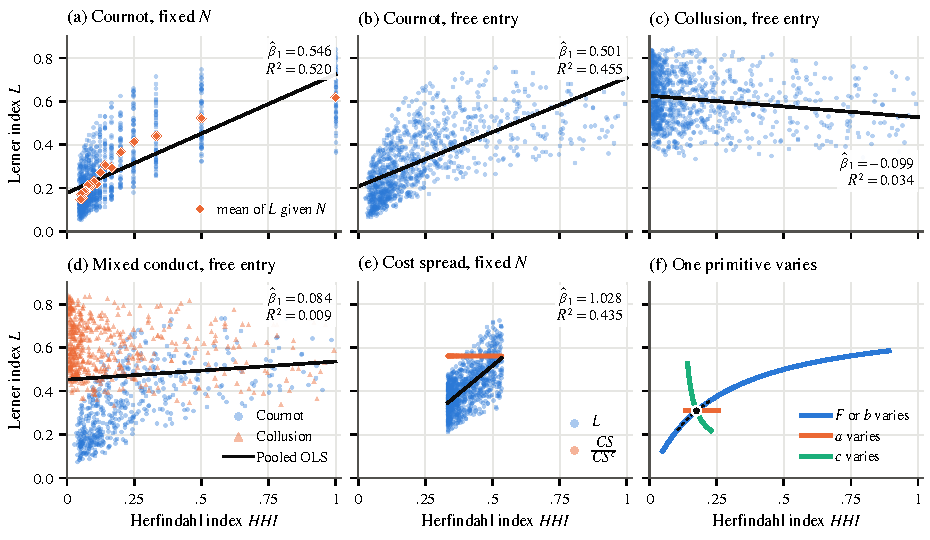
\includegraphics[width=\linewidth]{figures/ch01/scp_montecarlo.pdf}
\caption{Cross-industry SCP regressions on simulated industries. Each dot is an industry and each black
line is the OLS fit of the Lerner index on the Herfindahl index. Panel (a) also marks the mean margin at
each number of firms. Panel (d) separates Cournot and collusive industries. Panel (e) adds the consumer
surplus ratio $\frac{CS}{CS^c}$, which is the same in every industry. Panel (f) traces the free-entry
Cournot equilibrium as one primitive varies through the base point (black dot).}
\label{fig:01-montecarlo}
\end{figure}

Each of $n = 1{,}000$ industries has inverse demand $P = a - bQ$, marginal cost $c$ and fixed cost $F$.
The primitives are drawn independently, with $a \sim U[8, 12]$, $c \sim U[1, 4]$, $b \sim U[0.5, 2]$ and
$\ln F \sim U[\ln 0.1, \ln 10]$. We keep a draw only if the free-entry Cournot equilibrium has at least
one firm, which holds for 96.6 percent of draws. For each industry we compute the equilibrium
Herfindahl index and Lerner index under six designs.
\begin{enumerate}[label=(\arabic*)]
\item Cournot with a fixed number of firms $N \sim U\{1, \dots, 20\}$, drawn independently of the
primitives. Fixed costs are sunk, and in 64.4 percent of these industries the firms do not cover them.
\item Cournot with free entry, using \eqref{eq:01-fe-HL}.
\item Collusion with free entry, using \eqref{eq:01-collusion-fe}.
\item Mixed conduct with free entry, in which each industry colludes with probability $\frac{1}{2}$,
independently of its primitives.
\item Cost heterogeneity with a fixed structure. Each industry has $N = 3$ Cournot firms with marginal
costs $c_i = \bar c + \lambda (P - \bar c) z_i$, where $z = (-1, 0, 1)$ and the spread parameter
$\lambda \sim U[0, 0.95]$ is drawn independently of $(a, b, \bar c)$. The mean cost is
$\bar c \sim U[2.5, 4]$, which keeps every marginal cost positive.
\item One primitive at a time in Cournot with free entry, holding the others at the base point
$(a, c, b, F) = (10, 2.5, 1.25, 1)$.
\end{enumerate}
For designs (1) to (5) we estimate $L_k = \beta_0 + \beta_1 \HHI_k + e_k$ by OLS with
heteroskedasticity-robust standard errors in the HC1 form, which scales the White estimator by
$\frac{n}{n - 2}$. As a benchmark we compute the \emph{slope under random assignment}. It is the OLS slope of
the average causal curve $\frac{1}{n}\sum_k L_k(h)$ on $h$, with $h$ drawn from each design's own
distribution of the Herfindahl index. In designs (1), (2) and the Cournot half of (4), the causal curve of
industry $k$ is $L_k(h) = \frac{(a_k - c_k) h}{a_k h + c_k}$ (\cref{sec:01-cournot-hhi}). Under collusion it
is flat. In design (5), where concentration moves through the cost spread at fixed $N$, it is
$L_k(h) = \frac{h}{\varepsilon_k}$.
We also regress the consumer surplus ratio $\frac{CS}{CS^c}$, consumer surplus relative to its level at
price equal to (average) marginal cost, on the Herfindahl index. \Cref{fig:01-montecarlo} plots the
simulated industries and \cref{tab:01-montecarlo} reports the regressions.

\begin{table}[htbp]
\centering\small
\caption{Cross-industry OLS of the Lerner index on the Herfindahl index in 1,000 simulated industries}
\label{tab:01-montecarlo}
\begin{threeparttable}
\begin{tabular}{lccccc}
\toprule
 & \multicolumn{2}{c}{Cournot} & Collusion & Mixed & Cost spread \\
\cmidrule(lr){2-3}\cmidrule(lr){4-4}\cmidrule(lr){5-5}\cmidrule(lr){6-6}
 & Fixed $N$ & Free entry & Free entry & Free entry & Fixed $N = 3$ \\
 & (1) & (2) & (3) & (4) & (5) \\
\midrule
$\hat\beta_0$ & 0.178 & 0.208 & 0.625 & 0.453 & 0.003 \\
 & (0.004) & (0.005) & (0.005) & (0.009) & (0.016) \\
$\hat\beta_1$ & 0.546 & 0.501 & $-$0.099 & 0.084 & 1.028 \\
 & (0.022) & (0.020) & (0.016) & (0.022) & (0.042) \\
$R^2$ & 0.520 & 0.455 & 0.034 & 0.009 & 0.435 \\
Mean $\HHI$ & 0.179 & 0.238 & 0.174 & 0.206 & 0.398 \\
Mean $L$ & 0.275 & 0.327 & 0.608 & 0.470 & 0.412 \\
\midrule
Slope under random assignment & 0.535 & 0.594 & 0 & 0.340 & 1.036 \\
Slope of $\frac{CS}{CS^c}$ on $\HHI$ & $-$0.752 & $-$0.827 & 0 & $-$0.217 & 0 \\
 & (0.014) & (0.012) &  & (0.024) &  \\
\bottomrule
\end{tabular}
\begin{tablenotes}\footnotesize
\item Notes: 1,000 industries with $P = a - bQ$, marginal cost $c$ and fixed cost $F$. The primitives
$a \sim U[8, 12]$, $c \sim U[1, 4]$, $b \sim U[0.5, 2]$ and $\ln F \sim U[\ln 0.1, \ln 10]$ are drawn
independently and kept if the free-entry Cournot number of firms is at least one (96.6 percent of
draws). Column (1) draws $N \sim U\{1, \dots, 20\}$ independently of the primitives. Columns (2) to (4)
use the continuous free-entry number of firms. In column (4) each industry colludes with probability
$\frac{1}{2}$. Column (5) has 3 Cournot firms with costs $\bar c + \lambda (P - \bar c) z_i$,
$z = (-1, 0, 1)$, $\lambda \sim U[0, 0.95]$ and $\bar c \sim U[2.5, 4]$. HC1 standard errors in
parentheses. The slope under random assignment regresses the average causal curve
$\frac{1}{n}\sum_k L_k(h)$ on $h$, with $h$ drawn from the column's own distribution of $\HHI$.
$\frac{CS}{CS^c}$ is consumer surplus relative to its level at price equal to (average) marginal cost.
In columns (3) and (5) this ratio is the same in every industry, so its slope is exactly zero.
\end{tablenotes}
\end{threeparttable}
\end{table}

In design (1) the number of firms is independent of the primitives. Then $\E[L_k \mid \HHI_k = h] =
\E[L_k(h)]$, and OLS estimates the best linear approximation to the average causal curve. The estimate
$\hat\beta_1 = 0.546$ is close to the benchmark of $0.535$, and the difference is sampling error. Even here
the linear model is misspecified. Every causal curve passes through the origin and is concave
(\cref{fig:01-lerner-hhi}), and the mean margins in panel (a) trace this concavity. The fitted intercept
of $0.178$ is an artifact of fitting a line to a curve. The average derivative of the causal curves at the
observed concentrations is $1.452$, more than two and a half times the OLS slope. Most industries sit at low
concentration, where the curves are steep, while OLS gives much weight to the flat region at high
concentration.

In design (2) every industry lies on its causal curve, yet the OLS slope of $0.501$ falls about 16 percent
short of the random-assignment slope of $0.594$. The gap is the selection term of
\eqref{eq:01-potential-outcomes}. Industries become concentrated when $a - c$ is small relative to
$\sqrt{bF}$, and a small $a - c$ also lowers the causal curve $\frac{(a - c) h}{a h + c}$. The industries
observed at high concentration therefore have systematically lower curves, as in
\cref{ex:01-selection-elasticity}.

In design (3) every causal curve is flat, so concentration has no effect on margins at all. Yet OLS
reports a slope of $-0.099$ with a standard error of $0.016$. The negative sign comes from variation in
$a$ and $c$, which moves the two outcomes in opposite directions (\cref{tab:01-free-entry-cs}). Consumer
surplus is one quarter of its competitive level in every collusive industry, so concentration carries no
information about consumers either.

Design (4) mixes the two populations. The random-assignment slope is $0.340$, below the Cournot
benchmark because half of the causal curves are flat. The OLS slope is $0.084$, a quarter of the
benchmark, with an $R^2$ below one percent. Panel (d) of \cref{fig:01-montecarlo} shows why. Collusive
industries combine
high margins with low concentration and pull the pooled line toward zero.

Design (5) produces the strongest relation in the table, with $\hat\beta_1 = 1.028$ and $R^2 = 0.435$. The
benchmark slope is $1.036$, the mean of $\frac{1}{\varepsilon_k}$, because a wider cost spread raises
$L_k$ and $\HHI_k$ in the ratio $\frac{1}{\varepsilon_k}$ while leaving price unchanged. In this design the
benchmark curve comes from an intervention on the cost spread. It departs from
\cref{def:01-potential-margins}, since costs cannot stay fixed while concentration moves. In this narrower
sense the relation is causal. Yet price, output and consumer surplus are identical to those of the same industry
with symmetric costs, and $\frac{CS}{CS^c} = \frac{9}{16}$ in every industry. A researcher would see a
strong positive concentration-margin relation with no harm to consumers. \Cref{sec:01-demsetz} develops
this case.

Panel (f) isolates the comparative statics of \cref{tab:01-free-entry-cs}. Variation in $F$ or $b$ moves
the industry along an increasing concave curve, variation in $a$ moves it horizontally, and variation in
$c$ moves it down and to the right. The sign of the SCP slope depends on which primitive varies across
the sample. The slope is a property of the sample and says nothing about the technology of competition.
The fully
worked version of these models is in \cref{app:problems}.

\subsection{Panel data and fixed effects}\label{sec:01-salinger}

A natural response to omitted industry characteristics is to observe each industry several times and
remove what does not change. \citet{Salinger1990} reconsidered the concentration-margins relation with such
data. He used a Census of Manufactures panel of industries and restricted most of his analysis to
1972--84 \citep[p.~301]{Salinger1990}. Besides annual cross sections, he estimated the relation in long
differences, which remove time-invariant industry effects. The general fixed-effects version of the
regression is
\begin{equation}\label{eq:01-salinger}
\mathit{PCM}_{kt} = \alpha_k + \beta_1 \mathit{CR}_{kt} + \varphi^\top X_{kt} + e_{kt},
\qquad k = 1, \dots, n, \quad t = 1, \dots, T,
\end{equation}
where $\alpha_k$ is a fixed effect for industry $k$ and $\mathit{CR}_{kt}$ is a concentration ratio. The symbol
$\alpha_k$ is local to this subsection and differs from the price coefficient $\alpha$ of demand models. The
\emph{within estimator} subtracts each industry's time average from every variable:
\[
\mathit{PCM}_{kt} - \overline{\mathit{PCM}}_k = \beta_1 (\mathit{CR}_{kt} - \overline{\mathit{CR}}_k)
 + \varphi^\top (X_{kt} - \bar X_k) + (e_{kt} - \bar e_k),
\]
with $\overline{\mathit{PCM}}_k = \frac{1}{T}\sum_t \mathit{PCM}_{kt}$ and similarly for the other
variables. The transformation removes $\alpha_k$, and with it every time-invariant feature of the
industry, such as its demand elasticity, its technology or its accounting conventions.

With $T = 2$ the within estimator equals OLS on first differences, $\Delta \mathit{PCM}_k = \beta_1
\Delta \mathit{CR}_k + \varphi^\top \Delta X_k + \Delta e_k$. Salinger's long-difference regression has this
form without controls, plus a constant for the common change over the decade. Across 363 industries, he regressed the
change in margins from 1972 to 1982 on the change in $\mathit{CR}_4$, adjusted for market definition. The
slope is $0.178$, with a $t$-statistic of $3.49$ \citep[Table~4, row~1]{Salinger1990}. He notes that it is
roughly the size of his cross-sectional estimates \citep[p.~310]{Salinger1990}. He reads the similarity as
a sign that the cross-sectional relation could have evolved from changes in concentration over time
\citep[pp.~310--311]{Salinger1990}.

The cost is that identification now comes only from changes in concentration within an industry over
time. Consistency requires \emph{strict exogeneity}, $\E[e_{kt} \mid \mathit{CR}_{k1}, \dots,
\mathit{CR}_{kT}, X_{k1}, \dots, X_{kT}, \alpha_k] = 0$. Changes in concentration are responses to the
same demand and cost shocks that move margins. A demand boom raises margins and attracts entry, and a
cost shock can trigger exit or mergers. Such feedback violates strict exogeneity, as a simple model
shows.

\begin{example}[Entry feedback]\label{ex:01-feedback}
Let margin shocks $e_{kt}$ be independent over time with variance $\sigma_e^2$, and suppose the true
effect of concentration is $\beta_1$. Entry responds to last period's margin shock:
\[
\mathit{CR}_{kt} = \mathit{CR}_{k,t-1} - \zeta e_{k,t-1} + v_{kt}, \qquad \zeta > 0,
\]
with $v_{kt}$ independent noise of variance $\sigma_v^2$. In first differences, $\Delta \mathit{PCM}_{kt}
= \beta_1 \Delta \mathit{CR}_{kt} + \Delta e_{kt}$, where $\Delta \mathit{CR}_{kt} = -\zeta e_{k,t-1} +
v_{kt}$ and $\Delta e_{kt} = e_{kt} - e_{k,t-1}$. The two terms share $e_{k,t-1}$:
\[
\Cov(\Delta \mathit{CR}_{kt}, \Delta e_{kt}) = (-\zeta)(-\sigma_e^2) = \zeta \sigma_e^2 .
\]
With $\Var(\Delta \mathit{CR}_{kt}) = \zeta^2 \sigma_e^2 + \sigma_v^2$, the first-difference estimator
converges to
\[
\beta_1 + \frac{\zeta \sigma_e^2}{\zeta^2 \sigma_e^2 + \sigma_v^2} > \beta_1 .
\]
A favorable shock raises the margin today and attracts entry tomorrow, when the margin reverts.
Concentration and margins then fall together, and the estimator finds a positive relation even when
$\beta_1 = 0$.
\end{example}

Fixed effects also magnify measurement error. Most of the variation in concentration is between
industries and persists over time, while the within-industry changes are small. Noise in measured
concentration does not shrink in the same way. \citet{GrilichesHausman1986} make this point for panel
data in general, and the next proposition states it for the SCP regression.

\begin{proposition}[Attenuation of the within estimator]\label{prop:01-fe-attenuation}
Suppose $L_{kt} = \alpha_k + \beta_1 \HHI^*_{kt} + e_{kt}$ and we observe $\HHI_{kt} = \HHI^*_{kt} +
u_{kt}$. Industries are independent across $k$, and $T$ is fixed. The errors $u_{kt}$ are independent
across $k$ and $t$ with mean zero and variance $\sigma_u^2$, and independent of $\{\HHI^*_{ks}\}$,
$\{e_{ks}\}$ and $\alpha_k$. The shocks satisfy $\E[e_{kt} \mid \HHI^*_{k1}, \dots, \HHI^*_{kT}, \alpha_k] =
0$. Let $\sigma^2_{\tilde H} = \E\left[\frac{1}{T}\sum_t (\HHI^*_{kt} - \overline{\HHI}{}^*_k)^2\right] >
0$ be the within-industry variance of true concentration. As $n \to \infty$, the within estimator
converges to
\[
\beta_1 \, \frac{\sigma^2_{\tilde H}}{\sigma^2_{\tilde H} + \sigma^2_{\tilde u}}, \qquad
\sigma^2_{\tilde u} = \frac{T - 1}{T} \sigma_u^2 .
\]
\end{proposition}

\begin{proof}
Write $H_{kt} = \HHI_{kt}$ and $H^*_{kt} = \HHI^*_{kt}$, and write $\ddot y_{kt} = y_{kt} - \bar y_k$ for the
within transformation of any variable $y$. The fixed
effect drops out, so $\ddot L_{kt} = \beta_1 \ddot H^*_{kt} + \ddot e_{kt}$. The measured regressor
is $\ddot H_{kt} = \ddot H^*_{kt} + \ddot u_{kt}$. The within estimator is
\[
\hat\beta_1^W = \frac{\sum_k \sum_t \ddot H_{kt} \, \ddot L_{kt}}{\sum_k \sum_t \ddot H_{kt}^2}.
\]
Divide numerator and denominator by $nT$ and apply the law of large numbers across industries. The
numerator converges to
\[
\beta_1 \E\left[\frac{1}{T}\sum_t \ddot H^*_{kt} (\ddot H^*_{kt} + \ddot u_{kt})\right]
 + \E\left[\frac{1}{T}\sum_t \ddot H_{kt} \, \ddot e_{kt}\right] = \beta_1 \sigma^2_{\tilde H}.
\]
The cross term in $\ddot u_{kt}$ vanishes because $u$ is independent of $\HHI^*$. The second expectation
vanishes by strict exogeneity and the independence of $u$ and $e$. The denominator converges to
$\sigma^2_{\tilde H} + \E\left[\frac{1}{T}\sum_t \ddot u_{kt}^2\right]$. For each $t$,
\[
\E[\ddot u_{kt}^2] = \Var(u_{kt}) - 2 \Cov(u_{kt}, \bar u_k) + \Var(\bar u_k)
 = \sigma_u^2 - \frac{2\sigma_u^2}{T} + \frac{\sigma_u^2}{T} = \frac{T - 1}{T} \sigma_u^2 .
\]
Taking the ratio of the two limits gives the result.
\end{proof}

Compare the within estimator with a pooled regression that ignores the fixed effects and is valid only
if $\alpha_k$ is unrelated to concentration. Its reliability ratio is $\frac{\Var(\HHI^*)}{\Var(\HHI^*) +
\sigma_u^2}$, which uses the total variance of true concentration. The within estimator uses only the
within part. Normalize $\Var(\HHI^*) = 1$, and suppose 95 percent of it is between industries and
$\sigma_u^2 = 0.05$. The pooled reliability ratio is $\frac{1}{1.05} = 0.95$. With many periods, the
within ratio is $\frac{0.05}{0.05 + 0.05} = 0.5$, so the within estimator recovers only half of $\beta_1$.
Fixed effects remove one bias and enlarge another.

The lesson of this subsection holds for any such design. Industry fixed effects do not solve the
endogeneity of concentration, and where they remove one problem they create others: dynamic feedback
between margins and entry, and attenuation from measurement error.

\section{Efficiency, prices, and the afterlife of SCP}\label{sec:01-scp-after}

Suppose we found the econometric evidence credible: more concentrated markets have higher margins and
higher profits. Would that show that concentration is bad for consumers? This section takes up the
efficiency critique, the shift from profits to prices as the dependent variable, and the recent return of
cross-industry work in the debate over rising markups.

\subsection{Efficiency versus market power: the Demsetz critique}\label{sec:01-demsetz}

\citet{Demsetz1973} argued that concentration can be the result of superior efficiency or quality. Firms
with lower costs or better products grow, the industry becomes concentrated, and industry profits rise
because the efficient firms earn rents on their advantage. Consumers need not lose. On this view, which
became part of the Chicago critique of antitrust, the measurement may be correct while its normative
reading is wrong. \citet[p.~1013, fn.~2]{Bresnahan1989} summarizes the argument. ``Demsetz' alternative
interpretation was that high profits measure good performance, i.e.\ low costs, an argument he buttressed
by the observation that much of the profit in concentrated industries goes to large firms.'' Bresnahan
cites \citet{Demsetz1974} and notes that \citet{Bain1951} had already given a ``poor performance''
reading of the same observation. He describes the SCP literature as caught in ``a kind of gridlock'' over
whether high accounting profits signal good or bad performance \citep[p.~1013]{Bresnahan1989}.

The next proposition shows that the efficiency story holds exactly in the linear Cournot model with
heterogeneous costs.

\begin{proposition}[Concentration from cost differences]\label{prop:01-demsetz}
Let inverse demand be $P = a - bQ$, and let $N$ Cournot firms have constant marginal costs $c_1, \dots,
c_N$. Suppose all firms are active, $P > \max_i c_i$. Let $\bar c = \frac{1}{N}\sum_i c_i$ and
$\sigma_c^2 = \frac{1}{N}\sum_i (c_i - \bar c)^2$.
\begin{enumerate}[label=(\roman*)]
\item Output and price are $Q = \frac{Na - \sum_i c_i}{b(N + 1)}$ and $P = \frac{a + \sum_i c_i}{N + 1}$.
They depend on costs only through $\sum_i c_i$.
\item Shares are $s_i = \frac{P - c_i}{bQ}$, and $\HHI = \frac{1}{N} + \frac{N \sigma_c^2}{b^2 Q^2}$.
\item Industry variable profit is $\sum_i (P - c_i) q_i = bQ^2 \HHI$, and the share-weighted Lerner index
is $\sum_i s_i L_i = \frac{\HHI}{\varepsilon}$ with $\varepsilon = \frac{P}{bQ}$.
\end{enumerate}
\end{proposition}

\begin{proof}
(i) Firm $i$ maximizes $(a - bQ - c_i) q_i$. Its first-order condition is $a - bQ - b q_i - c_i = 0$, or
\[
b q_i = P - c_i .
\]
Sum over the $N$ firms: $bQ = NP - \sum_i c_i$. Substitute $P = a - bQ$:
\[
bQ = N(a - bQ) - \sum_i c_i \quad\Longrightarrow\quad bQ(N + 1) = Na - \sum_i c_i .
\]
Solve for $Q$ and substitute back into the demand curve:
\[
P = a - bQ = \frac{(N + 1)a - Na + \sum_i c_i}{N + 1} = \frac{a + \sum_i c_i}{N + 1}.
\]

(ii) The first-order condition gives $s_i = \frac{q_i}{Q} = \frac{P - c_i}{bQ}$. Because $\sum_i (P - c_i)
= bQ$, the mean of $P - c_i$ across firms is $\frac{bQ}{N} = P - \bar c$. Hence
\[
s_i - \frac{1}{N} = \frac{(P - c_i) - (P - \bar c)}{bQ} = \frac{\bar c - c_i}{bQ}.
\]
The variance of shares is $\sigma_s^2 = \frac{1}{N}\sum_i (s_i - \frac{1}{N})^2 = \frac{\sigma_c^2}{b^2
Q^2}$. By \cref{prop:01-hhi-variance}, $\HHI = \frac{1}{N} + N\sigma_s^2 = \frac{1}{N} + \frac{N
\sigma_c^2}{b^2 Q^2}$.

(iii) Using $P - c_i = b q_i$,
\[
\sum_i (P - c_i) q_i = b \sum_i q_i^2 = bQ^2 \sum_i s_i^2 = bQ^2 \HHI .
\]
Similarly, the Lerner index of firm $i$ is
\[
L_i = \frac{P - c_i}{P} = \frac{b q_i}{P} = \frac{bQ}{P} \, s_i = \frac{s_i}{\varepsilon}.
\]
Multiplying by $s_i$ and summing gives $\sum_i s_i L_i = \frac{\HHI}{\varepsilon}$.
\end{proof}

\begin{corollary}[A mean-preserving spread of costs]\label{prop:01-demsetz-spread}
Change the costs $c_i$ so that $\sum_i c_i$ is unchanged, $\sigma_c^2$ rises and all firms remain
active. Then price, output and consumer surplus $\frac{bQ^2}{2}$ are unchanged. The Herfindahl index,
industry variable profit and the share-weighted Lerner index all rise, and so does total surplus.
\end{corollary}

\begin{proof}
By \cref{prop:01-demsetz}(i), $P$ and $Q$ depend only on $\sum_i c_i$, so they and consumer surplus are
unchanged. With $Q$ fixed, part (ii) shows that $\HHI$ rises with $\sigma_c^2$. Part (iii) then shows that
industry profit $bQ^2\HHI$ and $\sum_i s_i L_i = \frac{bQ}{P}\HHI$ rise. Total surplus is consumer surplus
plus industry profit (gross of fixed costs), so it rises by the increase in profit.
\end{proof}

The corollary is the efficiency critique in one line. Across industries that differ only in the
dispersion of firm costs, concentration, margins and profits move together, and consumers are equally
well off in all of them. Design (5) of the Monte Carlo experiment is exactly this case.

\citet[Section~5.5]{Tirole1988} presents Demsetz's argument with two further examples. In Bertrand competition
with constant marginal costs, the lowest-cost firm charges the second-lowest cost and takes the whole market.
Concentration is then as high as any index that satisfies the axioms of \cref{rem:01-ej-axioms} allows, and the
firm earns a positive profit. With symmetric costs, concentration is lower and profit is zero.
\Cref{prop:01-more-draws} below studies this equilibrium when costs are random. Tirole's Exercise~5.7 is a
special case of \cref{prop:01-demsetz-spread}. Let demand be $Q = 1 - P$, so that $a = b = 1$, and let two
Cournot firms have costs $c_1 = c - d$ and $c_2 = c + d$ with $0 \le d$ and $c < 1$. The sum $c_1 + c_2 = 2c$
stays fixed as $d$ varies, and $\sigma_c^2 = d^2$. By \cref{prop:01-demsetz},
\[
  Q = \frac{2(1 - c)}{3}, \qquad P = \frac{1 + 2c}{3}, \qquad
  \HHI = \frac{1}{2} + \frac{2d^2}{Q^2} = \frac{1}{2} + \frac{9 d^2}{2(1 - c)^2} .
\]
Industry variable profit is
\[
  bQ^2 \HHI = \frac{Q^2}{2} + 2d^2 = \frac{2(1 - c)^2}{9} + 2d^2 .
\]
Both firms stay active as long as $P > c + d$, that is, $d < \frac{1 - c}{3}$. Over this range a wider cost
spread raises concentration and industry profit and leaves price unchanged.

Tirole draws a general lesson from such examples. Concentration indices give an easily computed indication of how
competitive an industry is. ``However, they have no systematic relationship with economic variables of interest
for assessing changes in cost, demand, or policy.'' With asymmetric firms, a given index need not be related in a
systematic way to welfare either. The indices are also endogenous, so their correlations with other variables
cannot be read as causal effects \citep[Section~5.5]{Tirole1988}.

The decomposition in part (ii) also shows that the source of concentration matters. Its first term,
$\frac{1}{N}$, reflects the number of firms. An extra active firm with cost $c_{N+1} < P$ lowers price,
because
\[
\frac{a + \sum_i c_i + c_{N+1}}{N + 2} < \frac{a + \sum_i c_i}{N + 1} = P
\quad\Longleftrightarrow\quad (N + 1) \, c_{N+1} < a + \sum_i c_i
\quad\Longleftrightarrow\quad c_{N+1} < P .
\]
Fewer firms therefore mean higher prices and lower consumer surplus. The second term reflects cost
dispersion, which leaves consumers unaffected. A single concentration index cannot tell the two apart.

The critique generated a large literature of firm-level \emph{horse-race regressions}. They include both
industry concentration and the firm's own market share:
\begin{equation}\label{eq:01-horse-race}
\pi_{ik} = \beta_0 + \beta_1 \mathit{CR}_k + \beta_2 s_{ik} + \varphi^\top X_{ik} + e_{ik},
\end{equation}
where $\pi_{ik}$ is the profitability of firm $i$ in industry $k$ and $s_{ik}$ its market share. The
efficiency view predicts $\beta_2 > 0$ with $\beta_1$ near zero, since large firms are profitable
because they are efficient. The market-power view predicts $\beta_1 > 0$, since concentration
facilitates high prices for all firms in the industry.

Demsetz stated the testable implication of his view himself (\citealp[p.~5]{Demsetz1973}, quoted in
\citealp[p.~46, n.~5]{LevensteinSuslow2006}). Suppose that efficiency is associated with concentration. Then
``there should be a positive correlation between concentration and the difference between the rate of return
earned by large firms and that earned by small firms.'' Let $\bar\pi^L_k$ and $\bar\pi^S_k$ be the average rates of return
of the large and the small firms in industry $k$. The implication concerns the cross-industry regression
\begin{equation}\label{eq:01-demsetz-test}
\bar\pi^L_k - \bar\pi^S_k = \gamma_0 + \gamma_1 \mathit{CR}_k + e_k ,
\end{equation}
and the efficiency view predicts $\gamma_1 > 0$. If concentration instead facilitates high prices for every firm
in the industry, the returns of small firms rise with concentration as well, and the gap need not widen. In
\eqref{eq:01-horse-race} the same contrast appears as $\beta_2 > 0$ against $\beta_1 > 0$.

Demsetz's own evidence fit the efficiency view. It was the observation, quoted above from
\citet[p.~1013, n.~2]{Bresnahan1989}, that much of the profit in concentrated industries goes to large firms.
\citet[p.~1142]{Hopenhayn1992} puts it more precisely: ``as reported by Demsetz (1973), more concentrated
industries could show higher profits for large firms and not for small ones.'' Hopenhayn also shows that the
pattern does not single out efficiency. In his competitive model of industry dynamics, a higher cost of entry
protects incumbents. It raises the profits of large firms but not necessarily those of small ones, and it raises
the market share of the largest firms. Industries with high entry costs then show the Demsetz pattern, although
every firm takes the price as given.

Later evidence was mixed. Studies that add the firm's own market share to the regression find that concentration
loses its effect \citep[Introduction, note~3]{Tirole1988}. \citet{Ravenscraft1983} reports evidence of
this kind from the line-of-business data of the Federal Trade Commission, for 3,186 business units in 258
manufacturing industries in 1975 \citep[p.~24]{Ravenscraft1983}. In the business-unit regressions of his
Table~1, the share coefficient is positive and significant. The concentration coefficient is small and negative, and significant in the generalized least squares
estimate \citep[Table~1]{Ravenscraft1983}. In the industry-level regression, which omits share, concentration has
a positive coefficient \citep[p.~26]{Ravenscraft1983}.
\citet{Schmalensee1985a} decomposed the variance of business-unit returns on assets in the 1975 line-of-business
data into industry, firm and share components. Firm effects were never statistically significant. Share effects
were significant but explained less than 1 percent of the variance. Industry effects explained about a fifth of
it, and at least 75 percent of the variance of industry average returns. About 80 percent of the variance was
unrelated to industry or share effects \citep[pp.~346--350]{Schmalensee1985a}.
Ravenscraft's paper focuses on the firm's share and Schmalensee's on the industry. Schmalensee finds the two
consistent, since share also explains less than 1 percent of the variance of profitability in Ravenscraft's
estimates \citep[p.~347]{Schmalensee1985a}. \citet[Section~5.5]{Tirole1988} and \citet[p.~46, n.~5]{LevensteinSuslow2006} point to
\citet{Schmalensee1987} for a test of collusion against differential efficiency.

The horse race cannot settle the question, because firm share is itself an equilibrium outcome. The model
of \cref{prop:01-demsetz} makes the point sharply. There, $L_{ik} = \frac{s_{ik}}{\varepsilon_k}$ for
every firm. In a sample of industries with a common elasticity $\varepsilon$, a regression of firm
margins on share and concentration returns $\beta_2 = \frac{1}{\varepsilon}$ and $\beta_1 = 0$ exactly.
Yet every firm prices above marginal cost because it internalizes the effect of its output on price,
which is market power by definition. The pattern ``$\beta_1 = 0$ and $\beta_2 > 0$'' is thus fully
consistent with a model in which firms exercise market power. It shows that margins line up with shares,
which the Cournot model of \cref{prop:01-cowling-waterson} predicts as well.

The argument has a modern echo. Dominant digital platforms attribute their large shares to the quality of
their products. Defendants have advanced this argument in recent monopolization cases. The logic is
Demsetz's: concentration may be high because some firms deliver more value per dollar, so the measured
concentration is fine and its normative reading is contested. Separating the two readings requires a
model of demand that values quality, which is the subject of \cref{ch:discrete,ch:blp}.

Efficiency and structure can also be jointly determined by competition itself. \citet{Syverson2004}
studies plants in the US ready-mixed concrete industry, where high transport costs make markets local.
Markets with denser demand have more plants, so buyers can switch between suppliers more easily. Less
efficient plants then find it harder to operate profitably, and the productivity distribution is
truncated from below. Denser markets have higher minimum and average productivity and less dispersion.
The causal arrow runs from demand density to both structure and efficiency, which no cross-industry
regression of performance on structure can capture.

\subsection{Price-concentration studies}\label{sec:01-price-concentration}

A later wave of studies replaced accounting profit with price as the dependent variable. They used
cross-sections of similar, geographically local markets within one industry
\citep[Section~3.5]{Bresnahan1989}. Examples include banking, for which \citet{Rhoades1982} lists dozens
of studies, and retail food \citep{Cotterill1986,Lamm1981}. Others cover gasoline \citep{Marvel1978},
airline city pairs \citep{GrahamKaplanSibley1983} and cement \citep{KollerWeiss1986}. \citet{Weiss1989} collected many such
studies. The estimating equation is typically a reduced form for price,
\begin{equation}\label{eq:01-price-concentration}
p_k = \beta_0 + \beta_1 \HHI_k + \varphi^\top X_k + e_k ,
\end{equation}
where $k$ now indexes local markets of one industry and $X_k$ contains demand and cost shifters. The
studies typically treat concentration as exogenous \citep[p.~1043]{Bresnahan1989}. They confirm a
positive relation between price and concentration, which is at least suggestive of market power
increasing with concentration. A variant uses changes in structure over time, as in the study of a
merger in the microfiche industry by \citet{BartonSherman1984}.

Price avoids the accounting problems of \cref{sec:01-accounting}, and similar local markets share many
omitted features. Yet the interpretation that concentration raises margins by changing conduct still
needs a defense. \citet[p.~1043]{Bresnahan1989} writes, ``I have seen no careful defense of this
interpretation, and I am troubled by it.'' He then lists difficulties which, in his words, ``have not
yet been rebutted.'' We state each one as an argument.
\begin{enumerate}[label=(\roman*)]
\item Free entry links price and concentration through scale, because larger markets fit more
firms. Take the free-entry Cournot model of \cref{sec:01-endogeneity} with $M$ consumers, so that
$b = \frac{1}{M}$. Then $P^* = c + \sqrt{\frac{F}{M}}$ and $\HHI^* = \frac{m^*}{a - c - m^*}$ with
$m^* = \sqrt{\frac{F}{M}}$, so both fall as $M$ grows. Firm output is $q^* = \frac{m^*}{b} = \sqrt{FM}$ and
average cost is $c + \frac{F}{q^*} = c + \sqrt{\frac{F}{M}} = P^*$. Firms in larger markets are larger,
have lower
average costs and break even everywhere. Price and concentration are related ``in a way that has no
obvious bad effects, and does not imply entry barriers'' \citep[p.~1044]{Bresnahan1989}.
\item Cost heterogeneity varies across markets with the same number of firms. Among such markets, the
more concentrated ones likely have more heterogeneous costs. By \cref{prop:01-demsetz}(ii),
concentration rises with $\sigma_c^2$ at fixed $N$. Cost heterogeneity may or may not interact with
conduct to raise prices.
\item Markets with more firms offer more draws on the lowest-cost firm, even if concentration is
exogenous. If that firm matters for price, price falls with the number of firms for purely
statistical reasons. \Cref{prop:01-more-draws} below formalizes the point.
\item Market-level data identify only an average of costs and conduct. Summing the first-order
conditions of \cref{prop:01-clarke-davies} with share weights gave the industry relation
\eqref{eq:01-industry-relation}. With marginal costs $mc_i$ that may vary across firms, the same steps
give Bresnahan's equation (17$'$) in our notation,
\begin{equation}\label{eq:01-avg-supply}
P = \overline{mc} - P'(Q) \, Q \, \theta, \qquad
\overline{mc} = \sum_i s_i \, mc_i, \qquad \theta = \sum_i s_i^2 (1 + r_i),
\end{equation}
which \cref{prop:01-supply-relation} derives in general. A lower price in
less concentrated markets can reflect a lower $\overline{mc}$, a lower $\theta$, or both. Most authors
have the second in mind. The two can also be linked, because a firm with a large cost advantage may
behave less competitively than it would against equal rivals.
\item The identity of the competitors matters as well as their number. \citet{GrahamKaplanSibley1983}
found that
airline city-pair markets served by carriers new to the industry have lower prices, all else equal.
These entrants very likely had
lower marginal costs, and their presence may also have changed the conditions of competition. ``Which is
it? The analysis of the paper cannot say'' \citep[p.~1044]{Bresnahan1989}. The same question applies to
the structure dummies in Porter's \citeyearpar{Porter1983} railroad cartel study.
\item Tests of the exogeneity of concentration have little power. \citet{GrahamKaplanSibley1983} tested the
exogeneity of their concentration measures and did not reject it. Their concentration coefficients
nevertheless changed
substantially when concentration was treated as endogenous. Bresnahan concludes that the test had little
power, so the assumption should not be taken as innocuous \citep[p.~1043, fn.~35]{Bresnahan1989}.
\end{enumerate}
Bresnahan stresses that these questions ``are not unanswerable'' and that the methods of
\cref{sec:01-identification} can tell marginal cost from conduct. ``The questions are, however,
unanswered'' \citep[p.~1044]{Bresnahan1989}. One clean exception he notes is \citet{SpillerFavaro1984}.
They study Uruguayan banking over a period that includes a change in entry regulation, and find that
freer entry shifts the supply relation down \citep[p.~1044, fn.~36]{Bresnahan1989}.

The more-draws argument can be made precise with order statistics, which \cref{app:math} reviews. Let
$c_{(k:N)}$ denote the $k$-th lowest of $N$ costs.

\begin{proposition}[More firms, more draws]\label{prop:01-more-draws}
Let the marginal costs of $N \ge 2$ firms be independent draws from a distribution $F_c$ on $[\underline
c, \bar c]$, and let firms compete in prices with a homogeneous good. In the equilibrium in which the
lowest-cost firm serves the market at the second-lowest cost, the price is $c_{(2:N)}$, and
\[
\E[c_{(2:N)}] = \underline c + \int_{\underline c}^{\bar c} G_N(x) \, \dd x, \qquad
G_N(x) \equiv \Pr(c_{(2:N)} > x) = (1 - F_c(x))^N + N F_c(x) (1 - F_c(x))^{N - 1}.
\]
The expected price is strictly decreasing in $N$ whenever $F_c$ is nondegenerate:
\[
\E[c_{(2:N)}] - \E[c_{(2:N+1)}] = \int_{\underline c}^{\bar c} N F_c(x)^2 (1 - F_c(x))^{N - 1} \, \dd x
> 0 .
\]
\end{proposition}

\begin{proof}
For a random variable $Y$ on $[\underline c, \bar c]$, $\E[Y] = \underline c + \int_{\underline c}^{\bar
c} \Pr(Y > x)\, \dd x$. The second-lowest cost exceeds $x$ exactly when at most one of the $N$ costs is
below $x$. No cost is below $x$ with probability $(1 - F_c(x))^N$. Exactly one is below $x$ with
probability $N F_c(x)(1 - F_c(x))^{N - 1}$. Adding the two gives $G_N(x)$. For the difference, write $F =
F_c(x)$ and compute
\begin{align*}
G_N(x) - G_{N+1}(x)
 &= (1 - F)^N \left[1 - (1 - F)\right] + F (1 - F)^{N - 1} \left[N - (N + 1)(1 - F)\right] \\
 &= F (1 - F)^N + F (1 - F)^{N - 1} \left[(N + 1)F - 1\right] \\
 &= F (1 - F)^{N - 1} \left[(1 - F) + (N + 1)F - 1\right] = N F^2 (1 - F)^{N - 1} .
\end{align*}
Integrating over $x$ gives the expression for the difference in expected prices. The integrand is
positive wherever $0 < F_c(x) < 1$, a set of positive length when $F_c$ is nondegenerate.
\end{proof}

The difference has a coupling interpretation. Adding a firm can only add a draw below $x$, so the event
``at most one cost below $x$'' becomes less likely. It fails exactly when one, and only one, of the first
$N$ costs is below $x$ and the new cost is also below $x$, which has probability
$N F_c(x)^2 (1 - F_c(x))^{N - 1}$. With costs
uniform on $[0, 1]$, $G_N(x) = (1 - x)^N + N x (1 - x)^{N - 1}$ and
\[
\E[c_{(2:N)}] = \int_0^1 (1 - x)^N \dd x + N \int_0^1 x (1 - x)^{N - 1} \dd x
 = \frac{1}{N + 1} + \frac{N}{N(N + 1)} = \frac{2}{N + 1}.
\]
The expected price is $\frac{2}{3}$ with two firms, $\frac{1}{2}$ with three and $\frac{1}{3}$ with five,
with identical Bertrand conduct in every market. In this stark model the lowest-cost firm serves the
whole market, so its share is one and the structural variable that varies is the number of firms present.
The same logic applies in any model in which the most efficient firms carry extra weight in price
determination.

\subsection{SCP today}\label{sec:01-scp-today}

SCP regressions survive as descriptive exercises. They are useful for laying out facts and empirical
regularities, such as which industries are concentrated and how margins and concentration move over
time. For the reasons in \cref{sec:01-scp-econometrics,sec:01-demsetz,sec:01-price-concentration}, they
are of little use for testing theories of market power. Schmalensee's own post-mortem concluded that the
cross-industry literature had not taught us much about how markets work
\citep[p.~160]{EinavLevin2010}.

A recent survey of health care markets restates the verdict \citep[p.~527]{HandelHo2021}. Handel and Ho note
that the SCP approach persisted longer in health economics than elsewhere. They summarize the reasons that
\citet{BerryGaynorScottMorton2019} give for the move away from it in the late 1980s. The first is measurement.
Markets are not observed directly in the data, and economic profits are hard to measure. The second is the
endogeneity of concentration. As a function of market shares, it is likely to be correlated with the unobserved
demand shifters that also move price. The third, and in their words the most fundamental, is that different
changes in primitives can produce the same correlation between concentration and prices. Mergers raise
concentration, markups and prices together and lower consumer surplus. Large firms with low marginal costs and
high fixed costs produce the same correlation, as in \citet{Demsetz1973}. So does a fall in search costs that
shifts share toward firms with high-quality products, which raises both concentration and consumer welfare
\citep{AutorEtAl2020}. The results of such regressions are therefore ``at best suggestive.'' Handel and Ho
conclude with the point of \citet{Bresnahan1989}. The effect of concentration can be studied only through three
objects: a demand system, the marginal costs of firms and the nature of oligopolistic competition.

Industry studies, the response described in \cref{sec:01-neio}, taught
much about particular industries, at the price of leaving cross-industry questions to other fields
(\cref{sec:01-today-debate}). The debate over rising markups and their role in rising inequality has
brought cross-industry, SCP-style work back, and the reactions within IO have been mixed.

\subsection{Rising markups and the production approach}\label{sec:01-rising-markups}

The recent cross-industry literature measures markups from production data instead of demand. The
approach goes back to \citet{Hall1988}, and \citet{DeLoeckerWarzynski2012} developed its firm-level
version. In this subsection $Q$ and $P$ denote the output and price of a single firm, and $\mu =
\frac{P}{mc}$ is the markup ratio of \cref{sec:01-lerner}.

\begin{proposition}[Markups from a flexible input]\label{prop:01-production-markup}
A firm produces $Q = f(V, K, \omega)$, where $V$ is a variable input bought at price $P^V$, $K$ collects
the other inputs and $\omega$ is productivity. Suppose the firm minimizes cost, takes $P^V$ as given,
and adjusts $V$ freely. Let $\lambda$ be the multiplier on the output constraint. Then $\lambda = mc$ and
\[
\mu = \frac{P}{\lambda} = \phi^V \frac{PQ}{P^V V}, \qquad
\phi^V = \frac{\partial f}{\partial V} \frac{V}{Q},
\]
where $\phi^V$ is the output elasticity of the variable input.
\end{proposition}

\begin{proof}
The firm chooses $V$ to minimize $P^V V$ plus the cost of the other inputs subject to $f(V, K, \omega) \ge
Q$. The Lagrangian is
\[
\mathcal{L} = P^V V + C^K(K) - \lambda \left[ f(V, K, \omega) - Q \right],
\]
where $C^K(K)$ is the cost of the other inputs. The first-order condition for $V$ is
\[
P^V = \lambda \frac{\partial f}{\partial V}.
\]
By the envelope theorem (\cref{app:math}), the derivative of minimized cost with respect to $Q$ equals
$\frac{\partial \mathcal{L}}{\partial Q} = \lambda$, so $\lambda = mc$. Multiply the first-order condition
by $\frac{V}{\lambda Q}$:
\[
\frac{P^V V}{\lambda Q} = \frac{\partial f}{\partial V} \frac{V}{Q} = \phi^V .
\]
Solve for $\lambda = \frac{P^V V}{\phi^V Q}$ and divide price by it:
\[
\mu = \frac{P}{\lambda} = \frac{P \phi^V Q}{P^V V} = \phi^V \frac{PQ}{P^V V}.
\qedhere
\]
\end{proof}

The formula needs no demand model and no assumption about conduct. The markup is the output elasticity
of a flexible input divided by that input's share of revenue. Its appeal for cross-industry work is
obvious, because revenue shares are available in accounting data for many firms.

\citet{DeLoeckerEeckhoutUnger2020} applied the formula to US publicly listed firms in the Compustat data from
1955 to 2016, treating cost of goods sold as the variable input. Each firm's markup is the ratio of its revenue
to its cost of goods sold, multiplied by an estimated output elasticity of the variable inputs. The method
follows \citet{DeLoeckerWarzynski2012}, and the firm markups are then averaged with revenue weights
\citep[p.~258 and n.~203]{AskerNocke2021}. As read from the figure in \citet[Figure~11, p.~259]{AskerNocke2021},
the revenue-weighted average markup rose from about 1.21 in 1980 to about 1.61 in 2016. The rise was confined to
the upper tail. The median markup is flat over the period, and in the authors' own words, ``Most firms see no
increase in markups. For the higher percentiles, markups increase. For the 90th percentile in particular, the
increase is sharpest. Between 1980 and 2016, it increases from 1.5 to 2.5'' (quoted in
\citealp[p.~258]{AskerNocke2021}). The rise in the average is thus ``largely driven by a few firms that currently
have much higher markups than decades ago.'' The finding drew wide attention because it suggested a rise in
market power across the economy. \citet{DeLoeckerSyverson2021} survey the production approach behind it, and
their chapter closes with its use to measure market power in product and labor markets
\citep[Preface, p.~xvi]{HoHortacsuLizzeri2021}.

The critiques mirror the problems of the SCP literature.
\begin{itemize}
\item The output elasticity $\phi^V$ must be estimated, usually from a production function by industry.
Most data record revenue instead of physical output. With revenue $R = PQ$ and profit maximization,
which sets marginal revenue $MR$ equal to $mc = \lambda$, the elasticity of revenue with respect to $V$ is
\[
\frac{\partial \ln R}{\partial \ln V} = \frac{\partial \ln R}{\partial \ln Q} \, \phi^V
 = \frac{MR}{P} \, \phi^V = \frac{\phi^V}{\mu}.
\]
Plugging this revenue elasticity into \cref{prop:01-production-markup} in place of $\phi^V$ gives
\[
\frac{\phi^V}{\mu} \cdot \frac{PQ}{P^V V} = \frac{\mu}{\mu} = 1
\]
for every firm. A revenue elasticity therefore carries no information about the markup, a point
developed by \citet{BondEtAl2021}.
\item A markup ratio above one must cover fixed and overhead costs (\cref{prop:01-zero-profit-markup}).
If technology has shifted toward fixed costs, such as software and overhead, $\mu$ rises with no rise in
profits. Which costs count as variable, cost of goods sold or also overhead, matters for the trend. A shift
of the population toward firms with larger fixed costs or lower costs of goods sold moves the average markup
by composition alone \citep[p.~258]{AskerNocke2021}. De Loecker, Eeckhout and Unger reply that the rise in
markups ``is not merely to offset a rise in overhead costs'' (quoted in \citealp[p.~258, n.~205]{AskerNocke2021}).
They find that markups rose by more than overhead costs, and that the excess markups are highest for the firms
with high overhead costs. Their measure of profits rose too, as did market value as a share of sales.
\item The average depends on the weights. A revenue-weighted mean rises when sales move toward large firms
with high markups, even if no firm's markup changes.
\item The relation between markups and concentration across industries is subject to every problem of
\cref{sec:01-scp-econometrics}.
\end{itemize}
Descriptive evidence on concentration itself gives a modern version of the Demsetz pattern of
\cref{sec:01-demsetz}. \citet{Ganapati2020} examines detailed firm-level Census data for 1972--2012. As reported
by \citet[p.~259]{AskerNocke2021}, increases in concentration are positively correlated with productivity and with real output growth. They are
uncorrelated with price changes and with overall payroll, and they are negatively correlated with labor's share
of revenue. Concentration rose where output and productivity grew, without the price increases that the
market-power reading would predict. This fits the efficiency reading better than the market-power reading,
although, as \cref{sec:01-demsetz} showed, it cannot rule out market power.

\citet{BerryGaynorScottMorton2019}, to whom \citet[p.~259, n.~206]{AskerNocke2021} point for an IO perspective on
this literature, develop the last point of the bulleted list above.
Their argument, summarized in \cref{sec:01-scp-today}, is that different changes in primitives can produce the
same correlation between concentration and markups, with very different positive and normative implications
\citep[p.~47]{BerryGaynorScottMorton2019}.
Following \citet{Bresnahan1989}, they hold that the effect of concentration cannot be interpreted without
demand, the marginal costs of firms and the nature of oligopolistic competition
\citep[p.~48]{BerryGaynorScottMorton2019}. They regard the production
approach as persuasive evidence that markups have risen, although the size and causes of the rise remain open
\citep[p.~49]{BerryGaynorScottMorton2019}.
Because industries are so heterogeneous, they argue that careful industry studies are also needed. They call
for many more such studies \citep[pp.~50 and 53]{BerryGaynorScottMorton2019}.

A demand-side study of one large industry models these three objects and reaches a contrasting answer.

\casehead{The US automobile industry}\citet{GriecoMurryYurukoglu2024}, GMY below, ask whether market power in the
US new-car market rose between 1980 and 2018, a period over which the production approach reports rising markups. We cite
the author manuscript on hand, whose title page is dated July 5, 2023. Its table and figure numbers may differ
from those of the published article.
Product data from Ward's Automotive give the sales, list prices and characteristics of new
cars and light trucks. An observation is a make-model-year, such as the 1987 Honda Accord, and the sample has
9,694 of them (Table~I). The market size is the number of US households divided by 2.5. The divisor reflects that
a household owns nearly two cars and keeps each for about five years. Survey data add the demographics of buyers
and the models they name as their second choices.

\casehead{Model and identification}Demand is a random coefficients logit of the kind developed in \cref{ch:blp}.
Household $i$ in year $t$ obtains from model $j$ the utility
\[
  u_{ijt} = x_{jt}\beta_i - \alpha_i p_{jt} + \xi_{jt} + \epsilon_{ijt}
\]
in our sign convention for price (their equation 1). The tastes $(\alpha_i, \beta_i)$ depend on demographics drawn
from the Current Population Survey and on normal taste shocks (equations 3 and 4). Manufacturers set the prices of
all their models in a static Nash-Bertrand game each year. The first-order conditions are those of
\cref{prop:01-multiproduct-foc} (their equation 6). GMY solve them for the marginal cost of every model at the
estimated demand parameters, as in \eqref{eq:01-implied-mc}. The price instrument is the real exchange rate of the
country where the model is built, lagged one year and taken from the Penn World Table. It moves with local labor
costs and with the nominal exchange rate, so it shifts the cost of supplying the US market. Average unobserved
quality and the value of the outside good both move the total share of new cars each year. The year effects alone
cannot separate them. GMY follow \citet{PakesBerryLevinsohn1993} and assume that, for models sold in two
consecutive years without a redesign, the change in $\xi_{jt}$ has mean zero (their equation 2).

Estimation is by the generalized method of moments (GMM) in three steps (their Section~5). The first matches micro moments, such as the average price paid
by each income quintile and the correlation of characteristics between first and second choices. The second
regresses the estimated mean utilities on characteristics, price, make and year dummies by two-stage least
squares with the exchange-rate instrument. The third applies the continuing-model restriction to the estimated
year effects. Standard errors come from a bootstrap of the micro data.

\begin{table}[htbp]
\centering
\caption{Markups, concentration and welfare in the US new-car market}
\label{tab:01-gmy}
\small
\begin{tabular}{@{}lrrl@{}}
\toprule
\multicolumn{4}{@{}l}{\textit{Panel A. Baseline estimates}} \\
\addlinespace[2pt]
 & 1980 & 2018 & Source \\
\midrule
Median Lerner index & 0.325 & 0.185 & Figure VIa, p.~2 \\
Share-weighted mean Lerner index & 0.42 & 0.22 & Table VII \\
Share-weighted mean Lerner index, log price & 0.32 & 0.27 & p.~21 \\
Herfindahl index (HHI points) & 2661 & 1132 & Table VII \\
Consumers' share of total surplus & 0.62 & 0.82 & p.~2 \\
\bottomrule
\end{tabular}

\medskip
\begin{tabular}{@{}lrr@{}}
\toprule
\multicolumn{3}{@{}l}{\textit{Panel B. Hypothetical cartels in 2018 (Table VII)}} \\
\addlinespace[2pt]
Cartel members & Mean Lerner index & HHI points \\
\midrule
None (2018 baseline) & 0.22 & 1132 \\
GM, Ford and Toyota & 0.26 & 2546 \\
Top three and Fiat & 0.35 & 3724 \\
Top four and Honda & 0.39 & 4819 \\
Top five and Nissan & 0.46 & 6000 \\
\bottomrule
\end{tabular}
\par\smallskip
\begin{minipage}{\textwidth}\footnotesize
\textit{Notes:} The Lerner index is $\frac{p - mc}{p}$, with marginal costs implied by Nash-Bertrand pricing.
Means are weighted by market shares. Total surplus is the sum of consumer surplus, producer surplus and deadweight
loss, which the authors call efficient surplus. In Panel B, parent companies join the cartel in order of 2018
sales, and Fiat is the parent of Chrysler. Source: Grieco, Murry and Yurukoglu (2024), author manuscript (title
page dated July 5, 2023), with the table, figure and page numbers of that manuscript.
\end{minipage}
\end{table}

\casehead{Results}\Cref{tab:01-gmy} collects the main numbers. The median Lerner index fell from 0.325 in 1980 to
0.185 in 2018, and the share-weighted mean fell from 0.42 to 0.22 (Figure~VIa and Table~VII). Markups fell across
the distribution, for every vehicle style and for imported as well as domestic models (Figures~VI and~VII). Demand
became more elastic. The share-weighted average own-price elasticity was $-4.23$ in 1985 and $-5.36$ in 2015, and
the market elasticity moved from $-1.07$ to $-1.29$ (Table~V). Concentration fell as well, and consumers gained.
The share of total surplus going to consumers rose from 0.62 to 0.82, and consumer surplus per household rose by
roughly \$8,000 (p.~2). GMY attribute the gain mainly to better product quality and better production technology.

Two checks address the main threats to this conclusion. With log price in utility in place of price, the mean
Lerner index still falls, from 0.32 to 0.27 (p.~21). The supply side assumes Nash-Bertrand pricing throughout, so
a move toward collusion could hide rising market power. Under fixed alternative conduct, collusion among the three
US manufacturers or among all firms, markups still decline (Figure~X). Panel~B of \cref{tab:01-gmy} asks how large
a cartel in 2018 would have to be to restore the 1980 mean of 0.42. Only a cartel of the six largest parent
companies exceeds it. GMY judge that a cartel of that scale would hardly escape the notice of antitrust
authorities (p.~27).

\casehead{Comparison with the production approach}GMY compare their series with the auto-industry estimates
of \citet{DeLoeckerEeckhoutUnger2020} in their Section~5.6 and Figure~XI. They also restate the
economy-wide rise from 1.21 to 1.61 in the sales-weighted ratio of price to marginal cost (p.~28), which matches
the figures above. The two auto series differ in level and in trend, although both are fairly flat after 1995. GMY
give three reasons why the production approach may fail in this industry. First, cost of goods sold includes fixed
manufacturing overhead under US accounting rules, so it is not the freely chosen input that
\cref{prop:01-production-markup} requires. Second, the output elasticity is estimated from revenue in place of
physical output, as in the critique of \citet{BondEtAl2021}. It is also pooled with firms in many other
manufacturing industries that share its two-digit code. Third, Compustat covers only listed firms. Several
manufacturers that sell in the US never appear in it, and its revenues include sales outside the US and of other
products.

The next example shows why a markup, even a correctly measured one, is a poor guide to welfare when products
improve.

\begin{example}[Quality, markups and consumer surplus]\label{ex:01-quality-markup}
This example follows \citet[p.~26, n.~13]{GriecoMurryYurukoglu2024}. A monopolist sells one product with constant
marginal cost $mc$ to $M$ consumers, who may instead choose an outside good. Consumer $i$ obtains utility
$\xi - \alpha p + \epsilon_{i}$ from the product and $\epsilon_{i0}$ from the outside good. The shocks are type-I
extreme value, and $\xi$ measures quality. Let $v = \xi - \alpha p$. The share of buyers and its price derivative
are
\[
  s = \frac{e^{v}}{1 + e^{v}}, \qquad \frac{\partial s}{\partial p} = -\alpha s (1 - s).
\]
The first-order condition $s + (p - mc)\frac{\partial s}{\partial p} = 0$ gives the dollar markup
\[
  p - mc = \frac{1}{\alpha (1 - s)} .
\]
Now raise quality and hold $mc$ fixed. Since $\dd s = s(1 - s)\,\dd v$ and $\dd v = \dd\xi - \alpha\,\dd p$,
differentiating the markup equation gives
\[
  \dd p = \frac{\dd s}{\alpha (1 - s)^2} = \frac{s}{\alpha (1 - s)}\left(\dd\xi - \alpha\,\dd p\right).
\]
Collect the terms in $\dd p$, using $1 + \frac{s}{1 - s} = \frac{1}{1 - s}$:
\[
  \frac{\dd p}{1 - s} = \frac{s}{\alpha (1 - s)}\,\dd\xi
  \quad\Longrightarrow\quad
  \frac{\dd p}{\dd \xi} = \frac{s}{\alpha} > 0 .
\]
The dollar markup rises one for one with price. The Lerner index rises too, because
\[
  \frac{\dd}{\dd \xi}\left(\frac{p - mc}{p}\right) = \frac{mc}{p^2}\,\frac{\dd p}{\dd \xi} > 0 .
\]
Yet the net utility of the product rises as well:
\[
  \frac{\dd v}{\dd \xi} = 1 - \alpha\,\frac{\dd p}{\dd \xi} = 1 - s > 0 .
\]
Consumer surplus is $\frac{M}{\alpha}\ln(1 + e^{v})$ up to a constant, by the log-sum formula of
\cref{sec:07-logsum}, so it rises with $v$. A better product raises the markup, by either measure, and consumer
surplus at the same time.
\end{example}

The data of GMY show the converse case. Better cars were also costlier to build. Over 1980 to 1999, average shares
and their price derivatives were stable while average prices rose (their Section~5.4.1 and Figure~VIII). For a
single-product firm the first-order condition gives
\[
  \frac{p - mc}{p} = -\frac{1}{p}\, s \left(\frac{\partial s}{\partial p}\right)^{-1}
\]
(their equation 7). Stable shares and derivatives keep the dollar margin fixed, so a higher price lowers the Lerner
index. A counterfactual that holds observed characteristics at their 1980 distribution removes the rise in
marginal cost and much of the fall in markups (Figure~IX). In both directions the lesson is the one GMY draw. A
markup is a poor measure of performance over long periods in which products change (p.~2). \Cref{ch:blp} develops
the model behind such studies, and \cref{app:problems} estimates simpler demand models on the replication data of
GMY.

The SCP paradigm and its critics leave one lesson for the rest of the book. Cross-industry correlations
between margins and concentration cannot separate demand, cost and conduct, because all three determine
both variables at once. The response is to study one industry at a time, with a model of its demand,
its costs and the conduct of its firms. \Cref{sec:01-neio} turns to that response.

\section{The New Empirical Industrial Organization}\label{sec:01-neio}

The cross-industry program of \cref{sec:01-scp} asked a single regression to separate demand, cost and conduct
across hundreds of industries. From the late 1970s the field moved in the opposite direction. Researchers studied
one industry at a time, wrote down an explicit model of its demand, cost and conduct, and estimated the conduct of
firms as a parameter. \citet{Bresnahan1989} named this program the \emph{New Empirical Industrial Organization}
(NEIO) and gave it its first systematic statement. This section presents the origins of the NEIO, its principles, its
workhorse model and its treatment of conduct. \Cref{sec:01-identification} then asks which features of the data
reveal market power. \Cref{fig:01-timeline} places the main contributions in time.

\begin{figure}[htbp]
\centering
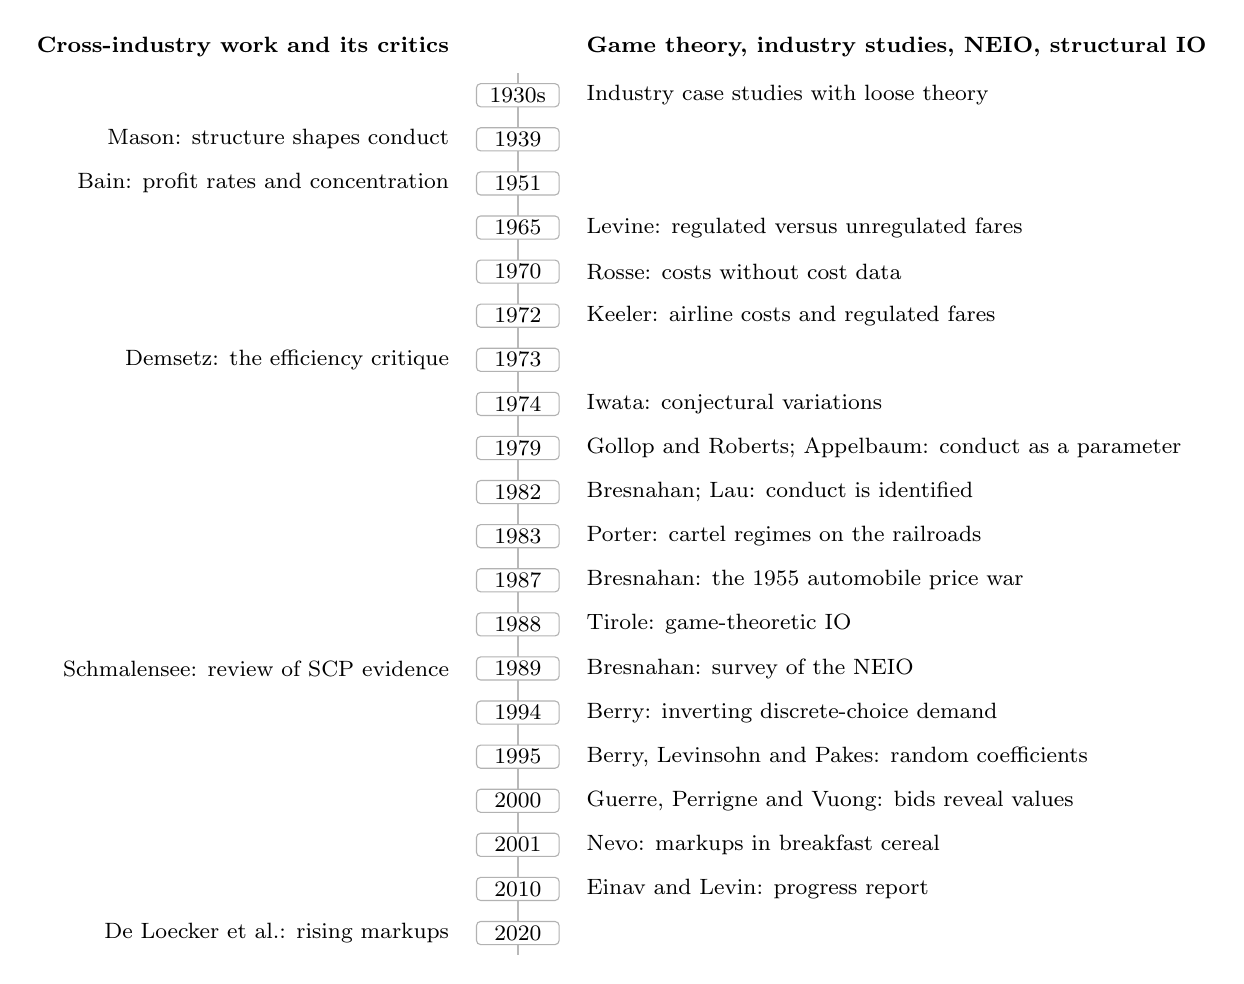
\begin{tikzpicture}[x=1cm, y=-0.56cm, every node/.style={font=\footnotesize}]
  \node[anchor=east, font=\footnotesize\bfseries] at (-0.75,-0.1) {Cross-industry work and its critics};
  \node[anchor=west, font=\footnotesize\bfseries] at (0.75,-0.1) {Game theory, industry studies, NEIO, structural IO};
  \draw[line width=0.8pt, gray!55] (0,0.5) -- (0,20.5);
  \foreach \y/\yr/\lt/\rt in {
    1/1930s//{Industry case studies with loose theory},
    2/1939/{Mason: structure shapes conduct}/,
    3/1951/{Bain: profit rates and concentration}/,
    4/1965//{Levine: regulated versus unregulated fares},
    5/1970//{Rosse: costs without cost data},
    6/1972//{Keeler: airline costs and regulated fares},
    7/1973/{Demsetz: the efficiency critique}/,
    8/1974//{Iwata: conjectural variations},
    9/1979//{Gollop and Roberts; Appelbaum: conduct as a parameter},
    10/1982//{Bresnahan; Lau: conduct is identified},
    11/1983//{Porter: cartel regimes on the railroads},
    12/1987//{Bresnahan: the 1955 automobile price war},
    13/1988//{Tirole: game-theoretic IO},
    14/1989/{Schmalensee: review of SCP evidence}/{Bresnahan: survey of the NEIO},
    15/1994//{Berry: inverting discrete-choice demand},
    16/1995//{Berry, Levinsohn and Pakes: random coefficients},
    17/2000//{Guerre, Perrigne and Vuong: bids reveal values},
    18/2001//{Nevo: markups in breakfast cereal},
    19/2010//{Einav and Levin: progress report},
    20/2020/{De Loecker et al.: rising markups}/%
  }{
    \node[fill=white, draw=gray!60, rounded corners=1.5pt, inner sep=1.6pt, minimum width=1.05cm] at (0,\y) {\yr};
    \node[anchor=east] at (-0.75,\y) {\lt};
    \node[anchor=west] at (0.75,\y) {\rt};
  }
\end{tikzpicture}
\caption[A timeline of empirical industrial organization]{A timeline of empirical industrial organization. Left:
the cross-industry tradition, its critics and its recent revival \citep{Mason1939,Bain1951,Demsetz1973,
Schmalensee1989,DeLoeckerEeckhoutUnger2020}. Right: game-theoretic IO, single-industry work, the NEIO and the
structural demand and supply models that followed \citep{Tirole1988,Levine1965,Rosse1970,Keeler1972,Iwata1974,
GollopRoberts1979,Appelbaum1979,Bresnahan1982,Lau1982,Porter1983,Bresnahan1987,Bresnahan1989,Berry1994,
BerryLevinsohnPakes1995,GuerrePerrigneVuong2000,Nevo2001,EinavLevin2010}. Rows are in chronological order and are
not drawn to scale.}
\label{fig:01-timeline}
\end{figure}

\subsection{Industry studies before the NEIO}\label{sec:01-early-studies}

Industry studies are older than the SCP paradigm. From the 1930s economists wrote detailed case studies of single
industries. These studies described pricing, capacity and rivalry with care. They made little attempt to generalize beyond the industry at hand, and the theory behind them was
loose. A case study could document that prices were high and stable. It could rarely say whether this reflected
market power, high costs or something else.

The clearest successes came in regulatory economics. \citet{Levine1965} compared air fares between Los Angeles
and San Francisco with fares in markets regulated by the Civil Aeronautics Board. Purely intrastate carriers on
this route, such as Pacific Southwest Airlines, were outside the Board's economic jurisdiction. The California
Public Utilities Commission, their only regulator, could not control entry in the period Levine studied
\citep[pp.~1430--1431]{Levine1965}. A state law signed on June 17, 1965, after Levine had written his article, gave the
Commission the power to regulate entry into intrastate air passenger service \citep[p.~1431, n.~63]{Levine1965}. The jet coach fare on this 350-mile route was about 3.9 cents per mile. The
national average jet coach fare was about 5.5 cents per mile, over longer stages that are cheaper to operate
\citep[p.~1433]{Levine1965}.
\citet{Keeler1972} estimated an airline cost function from interstate data and adjusted it to the operating
practices of the California intrastate carriers \citep[pp.~400--401]{Keeler1972}. He used seating densities
matching those of Pacific Southwest Airlines and a 60 percent load factor, below what the California carriers had
achieved \citep[pp.~405--406, 415 and 417]{Keeler1972}. The resulting
cost-based fares came within 3 percent of actual fares on two California intrastate routes. Among the 30 densest
routes in 1968, regulated coach fares exceeded these cost-based fares by 20 to 95 percent, and the markup tended
to rise with distance \citep[p.~416 and Table~6]{Keeler1972}. Both studies shaped the case for airline deregulation in the
late 1970s, the starting point of \cref{ch:airlines}. Their method compared prices with a competitive benchmark that
the data supplied directly, either an unregulated market or an estimate of cost.

\citet{Rosse1970} took a route that anticipated the NEIO. His title, which promises cost estimates ``without using cost
data'' (\cref{sec:01-lerner}), states the central idea of the later literature. He studied local newspapers, each treated as a
monopolist, and inferred marginal cost from the firm's pricing condition once demand had been estimated. The
application needed care because a newspaper sells two products. It sells circulation to readers and space to
advertisers, and the demand on each side depends on the other.

Let $Q^c$ denote circulation, $Q^a$ the column inches of advertising and $Q^e$ the column inches of editorial
content. The circulation price $P^c$ is the average price per subscription copy and the advertising price $P^a$ is
the average price per inch. Suppressing demand shifters and error terms, the inverse demands are
\begin{equation}\label{eq:01-rosse-demand}
P^a = P^a(Q^a, Q^c), \qquad P^c = P^c(Q^a, Q^c, Q^e).
\end{equation}
Advertisers pay more to reach more readers, so $\frac{\partial P^a}{\partial Q^c} > 0$. The newspaper chooses
$(Q^a, Q^c, Q^e)$ to maximize
\begin{equation*}
\Pi = P^a(Q^a, Q^c)\,Q^a + P^c(Q^a, Q^c, Q^e)\,Q^c - C(Q^a, Q^c, Q^e).
\end{equation*}
The marginal revenue of a product is the derivative of the firm's entire revenue with respect to that product's
quantity. For circulation, with $mc^c = \frac{\partial C}{\partial Q^c}$, the first-order condition is
\begin{equation*}
P^c + Q^c\frac{\partial P^c}{\partial Q^c} + Q^a\frac{\partial P^a}{\partial Q^c} - mc^c = 0 .
\end{equation*}
Solving for the circulation price gives the two-sided pricing condition \citep[eq.~6c]{Bresnahan1989}
\begin{equation}\label{eq:01-rosse-foc}
P^c = mc^c - Q^c\frac{\partial P^c}{\partial Q^c} - Q^a\frac{\partial P^a}{\partial Q^c} .
\end{equation}
The second term is the usual monopoly markup. The third term is new. It is the extra advertising revenue that one more
reader generates, and it lowers the circulation price. To see its size, divide \eqref{eq:01-rosse-foc} by $P^c$. Define
the inverse demand elasticities $f^c = -\frac{\partial \ln P^c}{\partial \ln Q^c} > 0$ and
$f^{ac} = \frac{\partial \ln P^a}{\partial \ln Q^c} > 0$. Then
\begin{align*}
\frac{P^c - mc^c}{P^c}
  &= -\frac{Q^c}{P^c}\frac{\partial P^c}{\partial Q^c} - \frac{Q^a}{P^c}\frac{\partial P^a}{\partial Q^c} \\
  &= f^c - \frac{P^a Q^a}{P^c Q^c}\cdot\frac{Q^c}{P^a}\frac{\partial P^a}{\partial Q^c}
   = f^c - \frac{P^a Q^a}{P^c Q^c}\, f^{ac} .
\end{align*}
The circulation price lies below marginal cost whenever $\frac{P^a Q^a}{P^c Q^c}\,f^{ac} > f^c$. This happens when
advertising revenue is large relative to circulation revenue and advertisers value readers highly. Most newspaper
revenue comes from advertising \citep[p.~1037]{Bresnahan1989}, so a reader price below marginal cost is a natural
outcome. A markup test applied to circulation alone would find price below marginal cost and could wrongly
conclude that newspapers have no market power. The theory of two-sided platforms later generalized this logic
\citep{RochetTirole2003,Armstrong2006}.

Rosse estimated the demand system \eqref{eq:01-rosse-demand} jointly with the pricing conditions. The
cross-equation restrictions between demand and marginal revenue then deliver marginal cost from the condition that
marginal cost equals marginal revenue. This let him treat marginal cost flexibly, for example by allowing transitory
shocks to firm size to separate short-run from long-run marginal cost. The approach is only as good as the estimated
marginal revenue. A linear demand curve may fit the data well and still give a poor estimate of its slope at the
observed point \citep[p.~1021]{Bresnahan1989}.

Two developments turned such isolated studies into a research program. The first was the critique of SCP regressions
developed in \cref{sec:01-scp-econometrics,sec:01-scp-after}. The second was the game theory revolution of the 1980s, which gave the field
sharp models of product differentiation, entry, pricing strategies and asymmetric information
\citep{Tirole1988}. Models proliferated so quickly that prominent members of the field lamented their overabundance
\citep{Fisher1989,Peltzman1991}. \citet[p.~146]{EinavLevin2010} note a lasting effect of this abundance. Because
predictions depended on fine details of preferences, information and commitment, empirical researchers learned to
take the institutional details of each market seriously. A single industry, studied with an explicit model, was the
natural place to do so.

\citet[Introduction]{Tirole1988} tells this history as two waves of interest in the field. The first was the
empirical Harvard tradition of \cref{sec:01-scp}. Alongside it, the ``Chicago tradition'' of Aaron Director and
George Stigler stressed rigorous theory and the empirical identification of competing theories. It also took a
permissive view of vertical restraints and predatory pricing, treating collusion as the main offense, and it
distrusted government intervention more than the Harvard tradition did. By the early 1970s many felt that theory
served more to explain statistical results or to buttress positions than to investigate markets systematically.
\citet[p.~273]{Joskow1975} wrote that ``the important messages are being carried by the informal theories,
stories, and behavioral observations.'' The formal models, in his phrase, were ``trotted out ex-post'' to show
that some formal apparatus could explain what was observed. Tirole attributes the second, mainly theoretical,
wave, which started in the 1970s, to three causes. On the demand side, researchers were dissatisfied with the
limits of cross-section work. On the supply side, leading theorists entered a field they had long ignored, and
noncooperative game theory became its standard tool. Game theory also made progress in two areas central to IO,
dynamics and asymmetric information. Tirole saw the new intra-industry studies of \citet{Porter1983} and
\citet{Bresnahan1987} as a sign that theory would soon feed back into empirical work (note~8).

\subsection{Principles of the NEIO}\label{sec:01-neio-principles}

\citet[p.~1012]{Bresnahan1989} summarizes the new approach in four ideas.
\begin{enumerate}
\item Price-cost margins are not observed. Economic marginal cost cannot be read from accounting data. The analyst
  infers it from firm behavior, uses differences between closely related markets to trace the effects of changes in
  marginal cost, or quantifies market power without measuring cost at all.
\item Industries have important idiosyncrasies. Institutional detail affects conduct, and it affects the measurement
  strategy even more. Comparative statics across industries are therefore suspect unless the markets are closely
  related.
\item Firm and industry conduct are unknown parameters. The behavioral equations by which firms set prices and
  quantities are estimated, and their parameters map into the notions of conduct of oligopoly theory.
\item The inference is explicit about its alternatives. The set of hypotheses is stated in advance. It includes the
  hypothesis of no strategic interaction, typically perfect competition, and the data can select it.
\end{enumerate}

The NEIO defined itself against three maintained hypotheses of the SCP paradigm \citep[pp.~1012--1013]{Bresnahan1989}.
The first was that economic price-cost margins can be observed in accounting data. The second was that
cross-industry differences in structure can be captured by a few observable measures, such as concentration ratios.
The third was that empirical work should estimate the reduced-form relation between structure and performance.
The gridlock over the meaning of high accounting profits, described in \cref{sec:01-demsetz}, showed where these
hypotheses led. No cross-industry regression could tell the market-power reading from the efficiency reading,
because both predict the same correlation.

The NEIO kept what the SCP paradigm had added to the field, namely systematic statistical evidence. It combined that
evidence with the attention to a single industry that marked the older case studies. In Bresnahan's words, the NEIO at
its best takes ``the best from the two great empirical IO traditions'' \citep[p.~1013]{Bresnahan1989}. A typical NEIO
paper is first of all an econometric model of one industry, with economic theory guiding both the specification and
the inference.

In practice these ideas translate into a recognizable research design.
\begin{itemize}
\item The unit of study is one industry, observed either as a time series or as a cross-section of geographic markets.
  Observations are similar to one another, so fewer factors are omitted than in a cross-section of industries.
\item Knowledge of the institutions guides the specification: which inputs matter, how the market clears, whether firms
  choose prices or quantities, and which prices are list prices and which are transaction prices.
\item Economic costs are inferred from pricing decisions rather than read from accounts. The inversion
  $\hat c = p\left(1 - \frac{1}{\hat\varepsilon^R}\right)$ of \cref{prop:01-infer-cost} is the simplest example.
\item Conduct is a parameter with an explicit interpretation (\cref{sec:01-conduct-parameter}).
\item External validity is claimed qualitatively. Some industries are studied as laboratories, for example ketchup,
  yogurt, laundry detergents or cement, and their value lies in mechanisms that travel to other markets. Others matter in
  their own right, for example health care, education, automobiles or airlines, and the specific numbers carry policy
  weight.
\end{itemize}
\citet[p.~147]{EinavLevin2010} make the same point about generality. The lasting lessons of industry studies tend to be
qualitative insights, such as the finding that entry can have large effects on prices, or methods that apply in many
settings.

A last principle concerns data. Economists in the field had long felt starved of appropriate data. The early NEIO
studies show this view to be false \citep[p.~1025]{Bresnahan1989}. The dissertations of Rosse, Bresnahan and Suslow
built their data from public industry sources, without relying on government statistics for the endogenous variables.
Porter's railroad data, discussed next, also came from industry records.

\subsection{Bresnahan's stylized model}\label{sec:01-stylized-model}

Most NEIO studies of homogeneous-good industries share one econometric structure. We present it in general form,
following \citet[Section~2.1]{Bresnahan1989} in the notation of this book, and then sketch Porter's study of a
railroad cartel as an illustration.

\casehead{Variables and equations}
Firms are indexed by $i = 1, \dots, N$ and observations, usually time periods, by $t$. The industry sells a single
product, so industry output $Q_t = \sum_i q_{it}$ is well defined. Demand has no intertemporal links from durability,
habits or learning. The endogenous variables are the market price $P_t$ and each firm's output $q_{it}$, or only
$Q_t$ when firm data are missing. Price-cost margins are not observed. The exogenous variables are demand shifters
$Y_t$, factor prices $W_{it}$ paid by firm $i$, and other cost shifters $Z_{it}$, such as fixed factors in a short-run
cost function. Three sets of unknown parameters describe demand ($\gamma$), cost ($\Gamma$) and conduct
($\vartheta$). The econometric errors $u^d_t$ and $u^c_{it}$ may enter nonlinearly and need not be scalars. The model
has five parts.
\begin{align}
P_t &= P(Q_t, Y_t, \gamma, u^d_t), \label{eq:01-bres-demand}\\
C_{it} &= C(q_{it}, W_{it}, Z_{it}, \Gamma, u^c_{it}), \label{eq:01-bres-cost}\\
mc_{it} &= C_q(q_{it}, W_{it}, Z_{it}, \Gamma, u^c_{it}), \label{eq:01-bres-mc}\\
P_t &= C_q(q_{it}, W_{it}, Z_{it}, \Gamma, u^c_{it}) - P_Q(Q_t, Y_t, \gamma, u^d_t)\, q_{it}\, \vartheta_{it}.
  \label{eq:01-bres-supply}
\end{align}
Equation \eqref{eq:01-bres-demand} is the inverse demand curve, \eqref{eq:01-bres-cost} the cost function and
\eqref{eq:01-bres-mc} marginal cost, where $C_q = \frac{\partial C}{\partial q}$. Equation \eqref{eq:01-bres-supply}
is the \emph{supply relation} of firm $i$, with $P_Q = \frac{\partial P}{\partial Q} < 0$ the slope of inverse
demand. Solving the demand equation and the $N$ supply relations together gives the reduced forms
\begin{equation}\label{eq:01-bres-rf}
P_t = P^*(W_t, Z_t, Y_t, \Theta, u_t), \qquad q_{it} = q_i^*(W_t, Z_t, Y_t, \Theta, u_t),
\end{equation}
where $\Theta = (\gamma, \Gamma, \vartheta)$ collects all parameters, $u_t$ all errors, and $W_t$ and $Z_t$ the
shifters of all firms. Equations \eqref{eq:01-bres-demand} to \eqref{eq:01-bres-rf} are Bresnahan's equations (1) to
(5) and (5$'$). We write $\Theta$ where Bresnahan writes $\Omega$, because $\Omega$ is the ownership matrix in this
book, and $\gamma$ where he writes $\delta$.

\casehead{The supply relation}
The supply relation states that marginal cost equals a ``perceived'' marginal revenue. For a monopolist,
$P + P_Q\,Q$ is marginal revenue. In \eqref{eq:01-bres-supply} the term $-P_Q\,q_{it}\vartheta_{it}$ is the wedge
between price and marginal cost, and $\vartheta_{it} \ge 0$ indexes how far the conduct of firm $i$ departs from price
taking. The value $\vartheta_{it} = 0$ is price taking. The value $\vartheta_{it} = 1$ is Cournot conduct and, with a
single firm, monopoly. Bresnahan calls it a supply relation because outside perfect competition firms have no
\emph{supply curve}, that is, no function $Q = S(P)$ that solves $P = mc(Q)$ \citep[fn.~6]{Bresnahan1989}. A firm
with market power chooses its output in response to the whole demand curve, including its slope, so the same price
can go with different outputs.

Equation \eqref{eq:01-bres-supply} seems to contain marginal cost, which the NEIO treats as unobserved. The
contradiction is only apparent. In the model, marginal cost is a function of the unknown parameters $\Gamma$, and it
can be computed only after $\Gamma$ has been estimated. Most methods estimate $\Gamma$ and $\vartheta$ in the same econometric step. A conduct parameter
that varies freely by firm and period would overparameterize the model. Bresnahan writes it this way only to nest all
known oligopoly theories, and every application restricts how $\vartheta_{it}$ varies.

\begin{remark}[Firm-level and industry conduct]\label{rem:01-firm-industry-conduct}
Bresnahan uses one symbol for two normalizations of conduct, and we keep them apart. The firm-level parameter
$\vartheta_{it}$ in \eqref{eq:01-bres-supply} equals $1 + r_i$ in the conjectural-variations notation of
\cref{sec:01-cournot-hhi}. It is $0$ for price taking, $1$ for Cournot and $N$ for symmetric collusion. The industry
parameter $\theta$ of this book weights each firm's conduct by its squared share, $\theta = \sum_i s_i^2\,\vartheta_i$,
as derived in \cref{prop:01-supply-relation} below. It is $0$ for price taking, $\HHI$ for Cournot and $1$ for collusion. With
symmetric firms, $q_{it} = \frac{Q_t}{N}$ and $s_i = \frac{1}{N}$, so
\begin{equation*}
\theta = \sum_{i=1}^{N} \frac{1}{N^2}\,\vartheta = \frac{\vartheta}{N}.
\end{equation*}
Symmetric Cournot ($\vartheta = 1$) gives $\theta = \frac{1}{N}$ and symmetric collusion ($\vartheta = N$) gives
$\theta = 1$, the convention used throughout the book.
\end{remark}

The core econometric methods are those for simultaneous equations, since $P_t$ and $q_{it}$ (or $Q_t$) are jointly
determined. Some studies estimate \eqref{eq:01-bres-demand} and \eqref{eq:01-bres-supply} directly as structural
equations, which is attractive because the conduct parameters are the object of interest. Studies that lack price,
quantity or firm-level data estimate reduced forms such as \eqref{eq:01-bres-rf} or aggregate the supply relations
to the industry level.

\subsubsection{An illustration: the Joint Executive Committee}\label{sec:01-porter-illustration}

\citet{Bresnahan1989} develops the stylized model alongside one application, Porter's (\citeyear{Porter1983}) study of
a nineteenth-century railroad cartel. We sketch that study here and draw out what it teaches about the NEIO. The full
case study, with the theory of \citet{GreenPorter1984} behind it and later reanalyses, appears in
\cref{ch:collusion-evidence}.

The Joint Executive Committee (JEC) was a legal cartel that controlled eastbound freight shipments from Chicago to the
Atlantic seaboard \citep[p.~302]{Porter1983}. Porter asks whether its prices switched between collusive and price-war
regimes, as trigger-price theories of collusion predict. The data are weekly records from the first week of 1880 to
the sixteenth week of 1886, which gives 328 observations. Quantity $Q_t$ is the tonnage of grain shipped by members,
and price $P_t$ is the grain rate in dollars per 100 pounds \citep[Table~2]{Porter1983}. Demand has constant
elasticity and shifts down when the Great Lakes are open to shipping. The supply relation is the industry version of
\eqref{eq:01-bres-supply}, derived in \cref{prop:01-supply-relation} below. Conduct takes a collusive value
$\theta^{c}$ in some weeks, and Porter normalizes conduct during price wars to the Bertrand value $\theta^{w} = 0$. He
treats each week's regime as an unobserved draw, collusive with a constant probability $\varpi$, and estimates the
system by maximum likelihood. We write $\varpi$ to keep $\pi$ for profit. Demand is inelastic, with an estimated
elasticity of $\hat\varepsilon = 0.80$ \citep[Table~3]{Porter1983}. With the lakes closed, predicted prices are 0.2780
dollars in collusive weeks and 0.1673 in price-war weeks \citep[Table~4]{Porter1983}. Collusion thus raised price by
66 percent and lowered quantity by 33 percent \citep[p.~310]{Porter1983}. The implied collusive conduct parameter is
$\hat\theta^{c} = 0.336$, which Porter calls roughly consistent with Cournot behavior \citep[p.~309]{Porter1983}.
\Cref{sec:13-jec} develops the model and estimates.

\citet[p.~1018]{Bresnahan1989} summarizes these findings in three statements. First, successful collusion raised
price by about 40 percent. This is the 0.40 reported for Porter in \cref{tab:01-bresnahan-table}. It measures the gap
from the collusive price, since $1 - \frac{0.1673}{0.2780} = 0.40$. Porter's 66 percent measures the same gap from
the price-war price. Second, the implied conduct was about as anticompetitive as Cournot. Only the gap between
the regimes is identified, because conduct during wars and the cost intercept enter the supply relation together. The
Cournot reading therefore rests on the unidentified assumption that price-war conduct was price taking (his
fn.~10). Third, the cartel broke down 28 percent of the time.

\casehead{What the illustration teaches}
Bresnahan sees three advantages in this structural approach \citep[p.~1018]{Bresnahan1989}. First, every parameter
has an economic meaning, so implausible estimates are diagnostic. Porter's demand elasticity is an example. With
$\hat\varepsilon = 0.80 < 1$, industry marginal revenue is negative, so the collusive weeks cannot reflect static joint
profit maximization \citep[p.~308]{Porter1983}. A conduct parameter of one would imply a Lerner index of
$\frac{1}{0.8} = 1.25$, which is impossible with positive marginal cost. Second, if the interpretation of conduct is
right, the link between the estimates and oligopoly theory is clear. Third, because the model is structural, the reason
why the data identify conduct can be stated. \Cref{sec:01-identification} takes up this third point.

Bresnahan also notes what the specification leaves out \citep[p.~1025]{Bresnahan1989}. A single constant probability
$\varpi$ tells us how often the cartel broke down. It cannot tell us what triggered breakdowns or what ended them,
which is where theories of collusion disagree. Answering that question needs a state-dependent switching probability.
Bresnahan doubts that the data can discriminate among the theories. A test of whether there are two regimes uses every
week of data, but a test of what starts and stops price wars has as many observations as there are price wars.

\subsection{Conduct as a parameter}\label{sec:01-conduct-parameter}

The stylized model treats conduct as an unknown parameter. This subsection derives the industry supply relation in
general form and lists the values of conduct implied by standard theories. It then surveys how the literature
specified conduct and explains how the estimates should and should not be read.

\begin{proposition}[Industry supply relation]\label{prop:01-supply-relation}
Consider a homogeneous good with differentiable inverse demand $P(Q)$, $P'(Q) < 0$, and $N$ firms with differentiable
costs $C_i(q_i)$. Firm $i$ chooses $q_i$ to maximize $P(Q)\,q_i - C_i(q_i)$, where $Q = q_i + Q_{-i}$ and the
conjectural variation $r_i = \frac{\dd Q_{-i}}{\dd q_i}$ of \cref{sec:01-cournot-hhi} is treated as a constant. Assume an interior solution
with every firm active, and let $mc_i = C_i'(q_i)$, $s_i = \frac{q_i}{Q}$ and $\varepsilon = -\frac{P}{Q\,P'(Q)}$.
Then:
\begin{enumerate}[label=(\roman*)]
\item Each firm satisfies the supply relation $P = mc_i - P'(Q)\,q_i\,(1 + r_i)$.
\item The industry satisfies
  \begin{equation}\label{eq:01-supply-relation}
  P = \overline{mc} - P'(Q)\,Q\,\theta, \qquad
  \overline{mc} = \sum_{i=1}^{N} s_i\, mc_i, \qquad
  \theta = \sum_{i=1}^{N} s_i^2 (1 + r_i).
  \end{equation}
\item Equivalently, $\frac{P - \overline{mc}}{P} = \frac{\theta}{\varepsilon}$, and average marginal cost can be
  recovered as $\overline{mc} = P + \theta\, Q\, P'(Q) = P\left(1 - \frac{\theta}{\varepsilon}\right)$.
\end{enumerate}
\end{proposition}

\begin{proof}
(i) The derivative of firm $i$'s profit is
\begin{equation*}
\frac{\dd}{\dd q_i}\Bigl[P(Q)\,q_i - C_i(q_i)\Bigr]
= P(Q) + q_i\,P'(Q)\,\frac{\dd Q}{\dd q_i} - C_i'(q_i)
= P + q_i\,P'(Q)\,(1 + r_i) - mc_i ,
\end{equation*}
because $\frac{\dd Q}{\dd q_i} = 1 + \frac{\dd Q_{-i}}{\dd q_i} = 1 + r_i$. Setting it to zero and solving for $P$
gives (i). (ii) Multiply (i) by $s_i$ and sum over $i$:
\begin{align*}
\sum_i s_i P &= \sum_i s_i\, mc_i - P'(Q)\sum_i s_i\, q_i (1 + r_i), \\
P &= \overline{mc} - P'(Q)\, Q \sum_i s_i^2 (1 + r_i),
\end{align*}
using $\sum_i s_i = 1$ and $q_i = s_i Q$. (iii) Subtract $\overline{mc}$ from both sides of \eqref{eq:01-supply-relation}
and divide by $P$:
\begin{equation*}
\frac{P - \overline{mc}}{P} = -\frac{Q\,P'(Q)}{P}\,\theta = \frac{\theta}{\varepsilon}.
\end{equation*}
Solving \eqref{eq:01-supply-relation} for $\overline{mc}$ gives the last statement.
\end{proof}

\Cref{prop:01-supply-relation} extends \cref{prop:01-clarke-davies} to marginal costs that vary with output. It shows
that one number, $\theta$, summarizes industry conduct for the purpose of the industry markup, whatever the
heterogeneity across firms. \Cref{tab:01-conduct-menu} lists the values implied by standard theories. The
inversion in part (iii) is the conduct-adjusted version of \cref{prop:01-infer-cost}. It is how the NEIO turns an
estimated demand curve and an assumed or estimated $\theta$ into an estimate of marginal cost.

\begin{table}[htbp]
\centering
\begin{threeparttable}
\caption{Conduct implied by standard oligopoly theories}
\label{tab:01-conduct-menu}
\small
\renewcommand{\arraystretch}{1.45}
\begin{tabular}{@{}lcccc@{}}
\toprule
Conduct & $r_i = \frac{\dd Q_{-i}}{\dd q_i}$ & $\vartheta_i = 1 + r_i$ & $\theta = \sum_i s_i^2(1 + r_i)$
  & $\frac{P - \overline{mc}}{P}$ \\
\midrule
Perfect competition & $-1$ & $0$ & $0$ & $0$ \\
Cournot & $0$ & $1$ & $\HHI$ & $\frac{\HHI}{\varepsilon}$ \\
Symmetric Cournot & $0$ & $1$ & $\frac{1}{N}$ & $\frac{1}{N\varepsilon}$ \\
Collusion (joint profit maximum) & $\frac{1 - s_i}{s_i}$ & $\frac{1}{s_i}$ & $1$ & $\frac{1}{\varepsilon}$ \\
Symmetric collusion & $N - 1$ & $N$ & $1$ & $\frac{1}{\varepsilon}$ \\
Clarke-Davies, $\kappa \in [0, 1]$ & $\kappa\frac{1 - s_i}{s_i}$ & $\frac{\kappa + (1 - \kappa)s_i}{s_i}$
  & $\kappa + (1 - \kappa)\HHI$ & $\frac{\kappa + (1 - \kappa)\HHI}{\varepsilon}$ \\
\bottomrule
\end{tabular}
\begin{tablenotes}\footnotesize
\item Notes: $s_i$ are output shares, $\HHI = \sum_i s_i^2$, and $\varepsilon$ is the market elasticity of demand.
Under collusion each firm acts as if rivals match its output in proportion to their shares, so
$1 + r_i = \frac{1}{s_i}$ and $\theta = \sum_i s_i = 1$. With constant marginal costs, the collusion rows require
equal costs across active firms. With rising marginal costs, they equalize marginal costs across firms. The
Clarke-Davies row is
\cref{prop:01-clarke-davies}: $s_i^2(1 + r_i) = (1 - \kappa)s_i^2 + \kappa s_i$, and summing gives
$\kappa + (1 - \kappa)\HHI$. Perfect competition requires rising marginal cost for an interior solution.
\end{tablenotes}
\end{threeparttable}
\end{table}

\subsubsection{How the literature specified conduct}\label{sec:01-conduct-taxonomy}

\citet[Section~2.2]{Bresnahan1989} sorts the early studies into four groups by how they wrote the supply relation. The
groups differ in language more than in substance.

\casehead{Supply relations from a single theory}
The first group derives $\vartheta_{it}$ from one explicit theory. The simplest case is monopoly or Cournot, where
$\vartheta_{it} = 1$ for all firms and periods \citep[eq.~6]{Bresnahan1989}:
\begin{equation*}
P_t = C_q(q_{it}, W_{it}, Z_{it}, \Gamma, u^c_{it}) - P_Q(Q_t, Y_t, \gamma, u^d_t)\,q_{it}.
\end{equation*}
With several firms this gives one estimating equation per firm. Rosse's newspapers, with the two-sided condition
\eqref{eq:01-rosse-foc}, belong here.

Bertrand pricing is the other static noncooperative model. With a homogeneous product and a flat marginal cost common to all firms
it is indistinguishable from perfect competition, so applications use differentiated products. \citet{Bresnahan1981}
estimates such a model on the 1977 and 1978 cross-sections of American automobiles. Products are ordered on a
one-dimensional quality index $\chi_j$, with neighbors $j - 1$ and $j + 1$. Consumers differ in a scalar taste for
quality. A consumer with taste $\nu$ who buys product $j$ at price $p_j$ gets $\nu\chi_j - p_j$, so she prefers $j$ to
$j + 1$ exactly when $\nu < \frac{p_{j+1} - p_j}{\chi_{j+1} - \chi_j}$. (Here $\nu$ is a taste for quality. Dividing
utility by $\nu$ gives the equivalent form with a consumer-specific price sensitivity used in \cref{ch:discrete}.) With
tastes spread uniformly with density $\gamma_0$, demand is
\begin{equation}\label{eq:01-vertical-demand}
q_j = \gamma_0\left(\frac{p_{j+1} - p_j}{\chi_{j+1} - \chi_j} - \frac{p_j - p_{j-1}}{\chi_j - \chi_{j-1}}\right) + u^d_j ,
\end{equation}
and quality is a hedonic function of observed characteristics $x_j$, such as length, weight and horsepower,
\begin{equation}\label{eq:01-vertical-quality}
\chi_j = f(x_j, \gamma_1) + u^{\chi}_j .
\end{equation}
These are Bresnahan's equations (7) and (8). Prices are manufacturer-to-dealer list prices, which equal transaction
prices for most sales, and quantities are model-year production. A firm $f$ owning the set of products
$\mathcal{J}_f$ chooses prices to maximize $\sum_{k \in \mathcal{J}_f} (p_k - mc_k)\,q_k$. Differentiating
\eqref{eq:01-vertical-demand},
\begin{equation*}
\frac{\partial q_j}{\partial p_j} = -\gamma_0\left(\frac{1}{\chi_{j+1} - \chi_j} + \frac{1}{\chi_j - \chi_{j-1}}\right),
\qquad
\frac{\partial q_{j+1}}{\partial p_j} = \frac{\gamma_0}{\chi_{j+1} - \chi_j},
\qquad
\frac{\partial q_{j-1}}{\partial p_j} = \frac{\gamma_0}{\chi_j - \chi_{j-1}} .
\end{equation*}
Let $\Omega_{jk} = 1$ if the same firm sells $j$ and $k$, and $\Omega_{jk} = 0$ otherwise. The matrix $\Omega$ is the
\emph{ownership matrix}, which returns in \cref{sec:01-workflow}. The first-order condition $q_j + \sum_{k \in \mathcal{J}_f}(p_k - mc_k)\frac{\partial q_k}{\partial p_j} = 0$ becomes
the supply relation
\begin{equation}\label{eq:01-vertical-foc}
q_j = \gamma_0 (p_j - mc_j)\left(\frac{1}{\chi_{j+1} - \chi_j} + \frac{1}{\chi_j - \chi_{j-1}}\right)
 - \Omega_{j,j+1}\,\gamma_0\,\frac{p_{j+1} - mc_{j+1}}{\chi_{j+1} - \chi_j}
 - \Omega_{j,j-1}\,\gamma_0\,\frac{p_{j-1} - mc_{j-1}}{\chi_j - \chi_{j-1}} ,
\end{equation}
the counterpart of Bresnahan's equation (6$''$). Marginal cost depends on the characteristics of the product. The
markup of product $j$ is large when its neighbors are far away in quality space. \citet{Bresnahan1981} finds large
price-cost margins on the larger cars, which are also much farther apart in quality space. The obvious weakness is the
restrictive demand system. Bresnahan probes it through the residuals, firm dummies and the quality error in
\eqref{eq:01-vertical-quality}. \Cref{ch:discrete} develops the vertical model in full.

A second class of single theories gives firms different roles. In the \emph{Stackelberg} model, firms
$2, \dots, N$ follow Cournot supply relations and the leader, firm 1, internalizes their reaction. Its supply relation is
\begin{equation}\label{eq:01-stackelberg}
P_t = C_q(q_{1t}, W_{1t}, Z_{1t}, \Gamma, u^c_{1t}) - P_Q(Q_t, Y_t, \gamma, u^d_t)\,q_{1t}\,(1 + \theta_S),
\end{equation}
where $\theta_S$ is the derivative of the followers' total output with respect to $q_1$, obtained by solving their
supply relations. A linear example shows what $\theta_S$ looks like. Let $P = a - bQ$ and let the $N - 1$ followers
have constant marginal cost $c$. Follower $j$'s Cournot condition is $a - bQ - b q_j = c$. Summing over the followers,
with $Q = q_1 + Q_F$ and $Q_F$ their total output,
\begin{align*}
(N - 1)(a - c) - (N - 1)\,b\,(q_1 + Q_F) - b\,Q_F &= 0, \\
Q_F &= \frac{(N - 1)(a - c - b\,q_1)}{N b}.
\end{align*}
Hence $\theta_S = \frac{\dd Q_F}{\dd q_1} = -\frac{N - 1}{N}$, and the leader's firm-level conduct is
$\vartheta_1 = 1 + \theta_S = \frac{1}{N}$. The leader behaves more aggressively than a Cournot firm because each unit
it adds displaces part of the followers' output.

The \emph{dominant-firm} model is closely related. \citet{Suslow1986} estimates it for Alcoa in the interwar period,
when Alcoa was the only producer of new aluminum and a fringe of firms recycled scrap. The fringe takes price as given,
so its supply relation is a supply curve. Write it as $Q_{ft} = S(P_t, W_{ft}, Z_{ft}, \Gamma, u^c_{ft})$, the inverse
of $P_t = C_q(Q_{ft}, \dots)$. Bresnahan's equations (10) and (10$'$) are these two forms. The dominant firm faces the
residual demand $q_1 = Q(P) - S(P)$, where $Q(P)$ is market demand. Its slope is
\begin{equation*}
\frac{\dd P}{\dd q_1} = \frac{1}{Q'(P) - S_P} = \frac{P_Q}{1 - P_Q S_P},
\end{equation*}
where $P_Q = \frac{1}{Q'(P)} < 0$ and $S_P = \frac{\partial S}{\partial P} \ge 0$. The first-order condition
$P + q_1\frac{\dd P}{\dd q_1} = mc_1$ can be written in the form of \eqref{eq:01-bres-supply}:
\begin{equation}\label{eq:01-dominant}
P_t = mc_{1t} - P_Q\,q_{1t}\,(1 + S_D), \qquad S_D = \frac{P_Q S_P}{1 - P_Q S_P} \in (-1, 0].
\end{equation}
These are Bresnahan's equations (11) and (11$'$). With no fringe response ($S_P = 0$) the leader is a monopolist on its residual demand and $S_D = 0$. As the fringe supply becomes
perfectly elastic, $S_D \to -1$ and the leader becomes a price taker. In elasticity form, with $s_1$ the leader's share
and $e_S$ the fringe supply elasticity, $P_Q S_P = -\frac{(1 - s_1)e_S}{\varepsilon}$, and
\begin{equation*}
\frac{P - mc_1}{P} = \frac{s_1}{\varepsilon}\,(1 + S_D) = \frac{s_1}{\varepsilon + (1 - s_1)\,e_S} .
\end{equation*}
In Suslow's data Alcoa's marginal cost is shifted by its accounting average variable cost, which does not enter the fringe
supply. The fringe supply is shifted by the stock of aluminum available for recycling. She estimates $S_D$ to be small, so
Alcoa had considerable market power despite the fringe \citep[p.~1023]{Bresnahan1989}. She identifies Alcoa as the
leader from the structure of the industry, a monopoly in new aluminum facing many recyclers.

Dynamic theories of collusion form the last part of this group. \citet{Stigler1964} argued that cartels held together
by self-interest should sometimes break down. Firms cannot always tell whether a fall in their sales reflects secret
price cutting, so suspicion leads to price wars even without cheating. \citet{GreenPorter1984} formalized this idea.
Firms observe the market price but not rivals' outputs, and a low price triggers a reversion to Cournot behavior for a
fixed period. The cartel chooses the collusive output, the trigger price and the length of punishment to maximize
expected profit. It does not push price to the monopoly level, because a higher price raises the gain from cheating.
\citet{AbreuPearceStacchetti1986} find more profitable designs in which both the start and the end of a price war are
triggered, so wars have random length and endogenous severity. \citet{RotembergSaloner1986} let demand fluctuate. When
current demand does not predict future demand, the gain from defecting is largest in booms, so the cartel must lower
its price in booms. All these theories imply that $\vartheta_{it}$ varies over time. They differ in the predicted
timing of the regimes, which is why Porter's constant $\varpi$ cannot tell them apart. \Cref{ch:collusion-theory}
develops these models.

\casehead{Testing a small set of theories}
A second group estimates the supply relations of a few distinct theories and tests among them.
\citet{Bresnahan1987} uses the vertical model \eqref{eq:01-vertical-demand} for the American automobile industry in
the mid-1950s. Under joint profit maximization, $\Omega_{jk} = 1$ for every pair of neighbors in
\eqref{eq:01-vertical-foc}, because industry marginal revenue counts every product. Under Bertrand pricing $\Omega_{jk}$
follows actual ownership.
Non-nested tests favor collusion in 1954 and 1956 and Bertrand competition in 1955, the year of a large expansion of
output and a fall in prices. A temporary breakdown of collusion thus explains part of the 1955 boom. \Cref{ch:discrete}
treats this paper as a case study. \citet{Geroski1983} and \citet{Roberts1984} test leader-follower theories on the
coffee-roasting data of \citet{GollopRoberts1979}. The smaller roasters behave as price-taking followers. The leading
firms behave less competitively than Cournot firms. They stop short of maximizing joint profits, even given the
fringe \citep[p.~1026]{Bresnahan1989}.

The difference between estimating a continuous $\vartheta$ and choosing among a few theories is purely econometric
\citep[p.~1026]{Bresnahan1989}. A researcher who estimates $\vartheta$ on a continuum tests theories with nested tests,
and may find a value between two theories. A researcher who specifies a few theories uses non-nested tests.

\casehead{Conjectural-variations language}
A third group writes conduct as a conjectural variation, a firm's ``expectation'' of how rivals' outputs respond
to its own. Starting with \citet{Iwata1974}, these papers write the supply relation as
\begin{equation}\label{eq:01-cv-supply}
P_t = C_q(\cdot) - P_Q(\cdot)\, q_{it}\,\bigl(1 + r_i(q_{it}, Q_{-i,t}, Z_{it}, \Phi)\bigr),
\end{equation}
where the parameters $\Phi$ let conjectures depend on firm size and other variables. Iwata asked where the Japanese
plate glass industry lay between competition and monopoly. He assumed, unlike most later work, that accounting data
reveal margins. \citet{GollopRoberts1979} let conjectures differ across firms in coffee roasting, and
\citet{SpillerFavaro1984} and \citet{GelfandSpiller1987} continued this emphasis on heterogeneous conduct in banking.

Equation \eqref{eq:01-cv-supply} differs from \eqref{eq:01-bres-supply} only in replacing $\vartheta_{it}$ by
$1 + r_i(\cdot)$. As a matter of logic the two are identical, since $\vartheta_{it} - 1 = r_i(\cdot)$ nests the same
models. Bresnahan puts it strongly: saying what the conjectural variation is and saying which theory of oligopoly holds
in the data are the same statement \citep[p.~1027]{Bresnahan1989}. The practical differences are two.
Conjectural-variation papers allow all values of $r_i$, and they stress the link between firm size and conduct.

\casehead{Aggregate data and average conduct}
A fourth group has only industry data. It writes the supply relation in aggregate form \citep[eq.~16]{Bresnahan1989},
\begin{equation}\label{eq:01-aggregate-supply}
P_t = C_q(Q_t, W_t, Z_t, \Gamma, u^c_t) - P_Q(Q_t, Y_t, \gamma, u^d_t)\, Q_t\, \theta_t ,
\end{equation}
as in \citet{Appelbaum1979} and Porter's study. Under the null of price taking ($\theta_t = 0$), $C_q$ is industry
marginal cost. With market power, firms generally have different marginal costs in equilibrium. Cournot firms with
different costs have different margins \citep{CowlingWaterson1976}, so a stable industry marginal cost curve need not
exist. \Cref{prop:01-supply-relation} gives the right reading. The aggregate $\theta_t = \sum_i s_{it}^2\vartheta_{it}$
weights each firm's conduct by its squared share, and $\frac{P - C_q}{P}$ is the share-weighted average markup. Some authors claimed that oligopoly theory implies identical
conduct across firms \citep{Appelbaum1982,Lopez1984}. Bresnahan rejects this claim, since nothing in oligopoly theory
forces firms to behave alike.

\subsubsection{What an estimated conjecture means}\label{sec:01-cv-warning}

The language of conjectures invites a misreading \citep[pp.~1027--1029]{Bresnahan1989}. Suppose we read
\eqref{eq:01-cv-supply} as the first-order condition of a firm that expects rivals' outputs to depend on its own:
\begin{equation}\label{eq:01-cv-profit}
\max_{q_i}\; P\Bigl(q_i + \sum_{j \ne i} Q_j(q_i)\Bigr)\, q_i - C(q_i),
\qquad
1 + r_i = \frac{\dd q_i}{\dd q_i} + \sum_{j \ne i} \frac{\dd Q_j}{\dd q_i} .
\end{equation}
For Cournot conduct ($r_i = 0$) and price taking ($r_i = -1$) the reading is harmless. A Cournot firm can be described as
expecting rivals' outputs to stay fixed, and a competitive firm as expecting price to stay fixed.

The trouble arises near collusion. Let all $N$ firms have the same costs and the collusive conjecture $1 + r_i = N$.
Each supply relation becomes
\begin{equation}\label{eq:01-collusive-foc}
P = C_q(\cdot) - P_Q(\cdot)\, N\, q_i ,
\end{equation}
which is the first-order condition for maximizing the joint profit of all $N$ firms. Read literally, $r_i = N - 1$ says
that each firm expects every rival to match any change in its output one for one, $\frac{\dd Q_j}{\dd q_i} = 1$. Repeated
games give a different account of the same outcome. Firms produce their share of the collusive output because they expect
a deviation to trigger a general breakdown of restraint. The matching behavior is never observed. It is the threat that
keeps it off the equilibrium path.

Bresnahan therefore separates two objects: (i) what firms believe will happen if they deviate, and (ii) what firms do
as a result of those beliefs. Estimated conjectures measure only (ii). If they are stable over time and breakdowns are
rare, they measure the average collusiveness of conduct. They carry no information about what would happen if one
firm expanded output on its own, which is the sense of ``conjectural variation'' in theoretical work. The only thing
they reveal about expectations is that the expectations suffice to deter departures from the normal arrangement
\citep[fn.~19]{Bresnahan1989}. For the same reason Bresnahan rejects reading the slope of $r_i(\cdot)$ in own output as
evidence of ``mutual forbearance''.

A second interpretive issue concerns firm size. Models with different conjectures for different size classes produce
an equilibrium size distribution even among identical firms. A competing explanation is that firms differ in cost.
Separating the two requires firm-specific cost functions, and in particular a comparison of the marginal costs of large
and small firms at the same output \citep[p.~1030 and fn.~20]{Bresnahan1989}.

\subsubsection{Every specification is a test of price taking}\label{sec:01-appelbaum}

\citet{Appelbaum1979} observed that setting every conduct parameter to zero in \eqref{eq:01-bres-supply}, or every
$r_i$ to $-1$, imposes price taking. Every specification of conduct, theoretical or not, therefore nests the
competitive model. Its estimation is a test of price-taking behavior, the title of Appelbaum's paper, against an
alternative in which firms raise price above marginal cost. This is the advance that the NEIO claims over the SCP
paradigm \citep[p.~1031]{Bresnahan1989}. When price taking is rejected, it is rejected against specific theories of
market power. The interpretation of the result is then clear, and only econometric problems can cloud the inference.

Two cautions carry over to later chapters. First, an estimated $\theta$ is a reduced summary of behavior, as the
discussion of conjectures shows. \citet{Corts1999} shows that when firms collude dynamically, the estimated $\theta$
tracks how the markup responds to demand shocks at the margin. It can then differ greatly from the average markup that
it is meant to measure. His Proposition~1 (p.~233) states the condition exactly, for linear demand, constant
marginal cost and a symmetric equilibrium. Let $q^*$ be equilibrium output per firm and $Y$ a demand shifter. The
estimate equals the elasticity-adjusted Lerner index that $\theta$ is meant to measure if and only if
\[
\frac{P - mc}{q^*} = \frac{\frac{\dd (P - mc)}{\dd Y}}{\frac{\dd q^*}{\dd Y}} .
\]
The margin per unit of output must equal the marginal response of the margin to output along demand-driven
movements. Under efficient supergame collusion this condition fails. The estimated conduct parameter then
understates market power unless demand shocks are fully permanent. When the shocks are completely transitory, it
may detect no market power at all, even if average margins are near the monopoly level (p.~245).
\Cref{ch:conduct} develops this critique. Second, the theory of the conduct parameter, including
its links to conjectural variations and pass-through, appears in \cref{ch:theory}.

\section{How the data identify market power}\label{sec:01-identification}

A structural model states the class of hypotheses among which the data choose. This makes a central question
answerable \citep[p.~1031]{Bresnahan1989}. Why do the data identify the inference of market power? Which implication
of perfect competition has been rejected when market power is measured? The question does not arise in the SCP
paradigm, which takes margins to be observed. In the NEIO margins are estimated, so we must ask which features of the
data and which natural experiments reveal them. Bresnahan distinguishes four classes of arguments: comparative statics
in demand, comparative statics in cost, direct estimation of marginal cost, and supply shocks. A fifth, comparative
statics in industry structure, is familiar in its logic but still lacked a sound identification argument in 1989. This
section explains each, then turns to differentiated products and to what the NEIO learned.

\subsection{The identification question}\label{sec:01-id-question}

The question is this. Given equilibrium prices and quantities from different but similar markets, under what conditions
can we identify conduct, or test for market power, without observing demand and cost? A linear model shows the
difficulty. Let demand and marginal cost be
\begin{equation}\label{eq:01-linear-id-model}
Q_t = a_0 + a_1 P_t + a_2 Y_t + u^d_t, \qquad mc_t = b_0 + b_1 Q_t + b_2 W_t + u^c_t ,
\end{equation}
with $a_1 < 0$, a demand shifter $Y_t$ and a cost shifter $W_t$. The slope of inverse demand is $\frac{1}{a_1}$, so the
supply relation of \cref{prop:01-supply-relation} is $P_t = mc_t - \theta\frac{Q_t}{a_1}$. Substituting marginal cost,
\begin{equation}\label{eq:01-linear-supply}
P_t = b_0 + \left(b_1 - \frac{\theta}{a_1}\right) Q_t + b_2 W_t + u^c_t .
\end{equation}
The cost shifter $W_t$ is excluded from demand, so it identifies $(a_0, a_1, a_2)$. The demand shifter $Y_t$ is
excluded from the supply relation, so it identifies $b_0$, $b_2$ and the slope $b_1 - \frac{\theta}{a_1}$. The two
parameters $b_1$ and $\theta$ enter only through this slope. A competitive industry with steep marginal cost and a
monopoly with flatter marginal cost produce the same data. When demand shifts out, price rises in both, either because
marginal cost rises with output or because of market power. Demand shifts that move the curve in parallel cannot tell
the two apart. \Cref{ch:conduct} develops this observational equivalence in detail, with figures, and shows how
\citet{Bresnahan1982} breaks it. The next subsection previews the general arguments.

\subsection{Five identification arguments}\label{sec:01-id-arguments}

\subsubsection{Comparative statics in demand}\label{sec:01-id-demand}

The first argument, due to \citet{Bresnahan1982} and \citet{Lau1982}, uses demand shifters that change the slope of
demand. \citet[Section~3.1]{Bresnahan1989} presents it in a simple version. Errors are additive, conduct $\theta$ is
constant, and the slope of inverse demand depends on the demand shifters but not on quantity. The demand equation and
the aggregate supply relation \eqref{eq:01-aggregate-supply} become
\begin{align}
P_t &= P(Q_t, Y_t, \gamma) + u^d_t, \label{eq:01-id-demand}\\
P_t &= C_q(Q_t, W_t, Z_t, \Gamma) + u^c_t - P_Q(Y_t, \gamma)\, Q_t\, \theta . \label{eq:01-id-supply}
\end{align}
Demand \eqref{eq:01-id-demand} has one endogenous regressor, $Q_t$, and the cost shifters provide instruments, so
$\gamma$ can be estimated. Call the estimate $\hat\gamma$ and form the constructed variable
$\hat P_{Q,t} = P_Q(Y_t, \hat\gamma)$. Then consider
\begin{equation}\label{eq:01-id-twostep}
P_t = C_q(Q_t, W_t, Z_t, \Gamma) + u^c_t - \hat P_{Q,t}\, Q_t\, \theta .
\end{equation}
Equations \eqref{eq:01-id-demand} to \eqref{eq:01-id-twostep} are Bresnahan's (17) to (19). Bresnahan calls the
two-step procedure too ugly for anyone to use, but it shows why better estimators identify $\theta$.

Equation \eqref{eq:01-id-twostep} has two endogenous variables: $Q_t$, which enters cost, and $\hat P_{Q,t}Q_t$, whose
coefficient is $\theta$. Two conditions are needed to estimate $\theta$. First, the two variables must not be
perfectly collinear. If the slope of demand does not depend on $Y_t$, then $\hat P_{Q,t}$ is a constant and
$\hat P_{Q,t}Q_t$ is proportional to $Q_t$. This is exactly the linear model above. Second, there must be instruments
for both endogenous variables. Both conditions hold when $Y_t$ has two elements, one that enters the slope $P_Q$ and one
that does not. A linear example is the inverse demand
\begin{equation*}
P_t = \gamma_0 + \gamma_1 Y_{1t} + (\gamma_2 + \gamma_3 Y_{2t})\, Q_t + u^d_t ,
\end{equation*}
in which $Y_{1t}$ shifts demand and $Y_{2t}$ rotates it. \citet{Lau1982} gives a general sufficient condition. The
parameter $\theta$ is identified if the inverse demand function cannot be written as $P(Q, Y) = \tilde P(Q, h(Y))$ for
a scalar index $h$. With a single demand shifter the index form holds trivially, with $h(Y) = Y$, so
identification requires at least two demand shifters.

\begin{remark}[Why a single demand index is not enough]\label{rem:01-lau}
Suppose $P(Q, Y) = \tilde P(Q, h(Y))$ with scalar $h$, and ignore errors. Fix $W$ and let $Q^*(h, W)$ be the
equilibrium quantity of a model with conduct $\theta > 0$ and marginal cost $C_q(Q, W)$. Assume $Q^*$ is strictly
monotone in $h$, with inverse $h = H(Q, W)$. Define a new marginal cost $mc^{\dagger}(Q, W) = \tilde P(Q, H(Q, W))$,
which depends only on cost variables. Consider a competitive industry with this marginal cost, and assume its
equilibrium is unique. For any $(h, W)$, the quantity $Q^*(h, W)$ satisfies $\tilde P(Q, h) = mc^{\dagger}(Q, W)$
because $H(Q^*(h, W), W) = h$. The competitive
model therefore reproduces every equilibrium of the model with market power, and $\theta$ is not identified without
restrictions on cost. With two demand shifters this construction fails. Two values of $Y$ can produce the same
equilibrium quantity with different slopes of demand. Competition then predicts the same price for both, while market
power predicts different prices.
\end{remark}

The economics is simple \citep[p.~1033]{Bresnahan1989}. Suppose the demand shifters could rotate the demand curve
around the equilibrium point. Under perfect competition nothing happens, because supply and demand still cross at the
same point. Under monopoly or any oligopoly theory, the change in the elasticity of demand shifts perceived marginal
revenue, and price and quantity respond. Market power has an idiosyncratic comparative static, and the data can detect
it.

Applications need a natural experiment that changes the slope of demand. In \citet{JustChern1980} the market power lies
on the buying side. A concentrated processing industry buys tomatoes from many farmers, and the adoption of a
mechanical harvester changed the elasticity of supply. The logic is the same as for sellers. In
\citet{Bresnahan1981,Bresnahan1987} elasticities depend on how close products are in quality space. More generally,
one shifter might measure the size of the economy, such as national income, and a second the price of a substitute.
The method stands or falls with the estimated demand elasticities. Critics offered other readings of the tomato
harvester, and the automobile results depend on the ordering of products in quality space.

A second route uses the structure of cost. Suppose marginal cost is homogeneous of degree one in factor prices, as it is
whenever it is derived from a cost function. Then every term of marginal cost involves a factor price. Any term in the
supply relation that does not involve a factor price must belong to the markup \citep[p.~1034]{Bresnahan1989}. For example, if
$C_q(Q, W) = \sum_k W_k\, g_k(Q)$, the supply relation
\begin{equation*}
P_t = \sum_k W_{kt}\, g_k(Q_t) - \theta\, Q_t\, P_Q(Q_t, Y_t, \gamma) + u^c_t
\end{equation*}
identifies $\theta$ from the one term that no factor price multiplies. This is how \citet{Appelbaum1979,Appelbaum1982}
obtained identification. The argument leans heavily on the functional form of marginal cost and on observing the true
marginal price of every input, capital in particular. The defense is robustness to other functional forms, to
quasi-fixed capital and labor, and to economic rather than accounting costs of capital. \Cref{ch:conduct} gives the
full treatment of identification through demand, with figures and estimation.

\subsubsection{Comparative statics in cost}\label{sec:01-id-cost}

\citet{PanzarRosse1987} propose two ideas. The first is to estimate a reduced form and to focus on the coefficients of
factor prices. The second is that a reduced-form revenue equation can be estimated even where price and quantity are
not observed. Let firm $i$'s equilibrium revenue be
\begin{equation}\label{eq:01-pr-revenue}
R_{it} = R^*(W_{it}, Z_{it}, Y_t, \Theta, u_t),
\end{equation}
obtained by solving demand and the supply relations for price and quantity and multiplying them. The
\emph{Panzar-Rosse statistic} is the sum of the elasticities of reduced-form revenue with respect to all factor prices,
\begin{equation}\label{eq:01-pr-stat}
\psi = \sum_k \frac{\partial R^*}{\partial W_k}\,\frac{W_k}{R^*} .
\end{equation}
Equations \eqref{eq:01-pr-revenue} and \eqref{eq:01-pr-stat} are Bresnahan's (20) and (21), where the statistic is
called $H_R$. It needs little data on endogenous variables, but it needs every variable that shifts cost or demand.
Revenue also avoids a quality correction. If the product is better in some markets, price per unit overstates the true
price there, but revenue is unaffected.

For an elementary monopolist, which chooses one quantity, $\psi$ has a definite sign. Let $R(Q, Y) = Q\,P(Q, Y)$ be
revenue as a function of output, so that $R_Q$ is marginal revenue. Let $Q^*(W)$ solve $R_Q(Q) = C_Q(Q, W)$, and let
equilibrium revenue be $R^*(W) = R(Q^*(W))$. Differentiating the first-order condition with respect to $W_k$,
\begin{equation*}
R_{QQ}\,\frac{\partial Q^*}{\partial W_k} = C_{QQ}\,\frac{\partial Q^*}{\partial W_k} + C_{QW_k}
\quad\Longrightarrow\quad
\frac{\partial Q^*}{\partial W_k} = \frac{C_{QW_k}}{R_{QQ} - C_{QQ}} .
\end{equation*}
Then $\frac{\partial R^*}{\partial W_k} = R_Q \frac{\partial Q^*}{\partial W_k}$. Because $C$ is homogeneous of degree
one in $W$, so is $C_Q$, and Euler's theorem gives $\sum_k W_k C_{QW_k} = C_Q$. At the optimum $C_Q = R_Q$. Hence
\begin{equation}\label{eq:01-pr-monopoly}
\psi = \frac{1}{R^*}\sum_k W_k\,R_Q\,\frac{C_{QW_k}}{R_{QQ} - C_{QQ}}
     = \frac{R_Q\,C_Q}{(R_{QQ} - C_{QQ})\,R^*}
     = \frac{(R_Q)^2}{(R_{QQ} - C_{QQ})\,R^*} \le 0 ,
\end{equation}
since the second-order condition requires $R_{QQ} - C_{QQ} < 0$. This is Bresnahan's equation (23). The intuition is
direct. A one percent increase in all factor prices raises marginal cost by one percent, and a monopolist's revenue
always falls when its costs rise. Otherwise its output was too large before the increase. \citet{PanzarRosse1987} show
that the result holds for a monopolist with many choice variables, including several outputs, quality or advertising.

A second hypothesis also has a sharp prediction. In long-run competitive equilibrium with free entry, every firm
produces at the minimum of its average cost. A proportional increase in all factor prices raises minimum average cost in
the same proportion and leaves the efficient scale unchanged. Firm revenue, the product of the two, rises in the same
proportion, so $\psi = 1$. Industry output falls through exit. In this case demand shifters should not enter the
revenue equation, which gives a second testable restriction \citep[p.~1037 and fn.~30]{Bresnahan1989}.

The statistic does not discriminate perfectly. It need not be positive when firms are not monopolists, although
\citet{PanzarRosse1987} show that it is positive in some models of oligopoly and monopolistic competition. A negative
$\psi$ can also arise for reasons other than monopoly, so false findings of monopoly are possible. The applications
use cross-sections of similar local markets. \citet{PanzarRosse1977} study newspapers in local media markets and reject
monopoly even for newspapers that are alone in their market, which points to competition from other media.
\citet{Shaffer1982} studies banks in New York State in 1979 and rejects both monopoly and long-run competition. These
studies are convincing to the extent that the cross-section reflects long-run equilibria and every cost shifter is
measured and correctly entered. \Cref{ch:conduct} proves the results above and discusses the test further.

A per-unit tax is the cleanest cost shifter, because it enters marginal cost one for one and is observed.
\citet{Sumner1981} builds a test of monopoly pricing on state cigarette excise taxes. Let a firm face a residual
demand elasticity $\varepsilon^R > 1$ that is constant over the sample. Its marginal cost is $mc = X\phi + E + R$,
where $X$ contains observed cost factors, $E$ unobserved ones and $R$ the tax per pack. Marginal revenue equals
marginal cost when
\[
P = \frac{\varepsilon^R}{\varepsilon^R - 1}\, mc
\]
(his equations 1 and 2, with his elasticity $\eta = -\varepsilon^R$). Multiplying out and absorbing the factor
$\frac{\varepsilon^R}{\varepsilon^R - 1}$ into the coefficients of $X$ gives his estimating equation (4), for
state $i$ in year $t$,
\begin{equation}\label{eq:01-sumner}
P_{it} = X_{it}\phi + \rho R_{it} + U_{it}, \qquad \rho = \frac{\varepsilon^R}{\varepsilon^R - 1} = \frac{P}{mc} .
\end{equation}
Sumner calls the tax coefficient $\theta$. We write $\rho$ because the coefficient is a pass-through rate that
equals the ratio of price to marginal cost. It differs from the conduct parameter $\theta$ of
\cref{sec:01-conduct-parameter}. Competition with constant marginal cost implies $\rho = 1$. The data
are 1,200 state-years, for 47 states and the District of Columbia over 1954--1978, and the estimator is OLS. With
state and year dummies in $X_{it}$, $\hat\rho = 1.074$ (0.013). With the national consumer price index in place of
the dummies, $\hat\rho = 1.029$ (0.011), and a variance-components model gives $1.069$ (0.013) (Table~1,
p.~1017). Sumner reports implied firm elasticities of 13.5, 34.5 and 14.5 in absolute value. Every estimate is
significantly above one, so atomistic competition is rejected. Yet the firm elasticities lie far above the
industry elasticities of 0.3 to 0.8 found in other studies (p.~1017), so an effective cartel is rejected too.
The reported elasticities equal $\frac{1}{\hat\rho - 1}$, and \cref{ch:conduct} compares them with the exact
inversion of \eqref{eq:01-sumner} in its full treatment of the paper.

\citet{Sullivan1985} and \citet{AshenfelterSullivan1987} extend the idea to settings where market price and quantity
are observed. Let all firms share a constant marginal cost $c$, and let firm $i$ satisfy the supply relation
$P = c - P'(Q)\,q_i\,(1 + r_i)$. Solving for output and summing over firms,
\begin{equation*}
q_i = \frac{P - c}{-P'(Q)\,(1 + r_i)}
\quad\Longrightarrow\quad
Q = \frac{P - c}{-P'(Q)}\sum_i \frac{1}{1 + r_i}
  = (P - c)\,\frac{\varepsilon\, Q}{P}\sum_i \frac{1}{1 + r_i},
\end{equation*}
using $-\frac{1}{P'(Q)} = \frac{\varepsilon Q}{P}$. Dividing by $Q$ gives $\sum_i (1 + r_i)^{-1} = \frac{1}{\varepsilon L}$,
where $L = \frac{P - c}{P}$. Now let $E_P = \frac{\dd \ln P}{\dd \ln c}$ and $E_Q = \frac{\dd \ln Q}{\dd \ln c}$ be the
elasticities of the reduced forms with respect to marginal cost. A cost shift moves the equilibrium along a fixed demand
curve, so $\varepsilon = -\frac{E_Q}{E_P}$. Hence
\begin{equation}\label{eq:01-sullivan}
\sum_i \frac{1}{1 + r_i} = -\frac{E_P}{E_Q\, L} \;\ge\; -\frac{E_P}{E_Q} ,
\end{equation}
where the inequality uses $L \le 1$, which holds when marginal cost is nonnegative. Bresnahan's equation (25) states the
first relation as a weak inequality, which is all the test needs. The left side equals $1$ under collusion, $N$ under
Cournot and infinity under perfect competition. The right side can be estimated from cost shifts alone. If
$-\frac{E_P}{E_Q}$ exceeds one, the data reject collusion. No value of the bound can reject competition. Sullivan uses a
panel of American states and years for cigarettes, with state excise taxes as the cost shifter. Assuming that costs are
at least as large as taxes tightens the bound, and he rejects the hypothesis that prices are set as if by a cartel.
\citet{AshenfelterSullivan1987} use year-to-year tax changes within a state in a nonparametric version. Their tests
indicate that monopoly and the other simple models without at least a moderate amount of competition predict
poorly how excise tax changes affect cigarette prices, sales and revenues (p.~483). They also find some evidence
that tax increases do not consistently raise prices and lower sales. The main
questions are whether the cost shifters proxy for other variables and whether their link to marginal cost is known.
Taxes are strong on the second count.

Why do cost shifts give only inequalities while demand shifts can deliver an estimate of conduct
\citep[p.~1039]{Bresnahan1989}? The conduct parameter lives in the supply relation. A demand shift traces out the supply
relation, which is the object we want. A cost shift traces out the demand curve. It sheds light on the supply relation
only indirectly.

\subsubsection{Estimating marginal cost more directly}\label{sec:01-id-factor}

The previous arguments use only price and quantity as endogenous variables. A third approach estimates marginal cost
from cost or factor-demand data, using the duality between cost and production \citep[Section~3.3]{Bresnahan1989}.
\citet{GollopRoberts1979} and \citet{Appelbaum1979,Appelbaum1982} add the demands for inputs, typically labor, capital
and materials, to the system. By Shephard's lemma (\cref{app:math}) the factor demands are the derivatives of the cost
function with respect to factor prices. With $X_{it}$ the vector of input demands, the system is
\begin{align}
P_t &= P(Q_t, Y_t, \gamma, u^d_t), \notag\\
P_t &= C_q(q_{it}, W_{it}, Z_{it}, \Gamma, u^c_{it}) - P_Q(Q_t, Y_t, \gamma, u^d_t)\, q_{it}\,\vartheta_{it},
  \label{eq:01-factor-system}\\
X_{it} &= C_W(q_{it}, W_{it}, Z_{it}, \Gamma, u^c_{it}), \notag
\end{align}
Bresnahan's equations (26) to (28). The cost parameters $\Gamma$ appear in both the supply relation and the factor
demands. Because $C$ is homogeneous of degree one in $W$, the factor demands taken together depend on all its parameters.
Every parameter of marginal cost is then estimated from the factor demands, and the supply relation is left to identify
conduct.

A Cobb-Douglas example makes this concrete. Let $C(q, W) = A\, q^{\frac{1}{\rho}}\prod_k W_k^{\beta_k}$ with
$\sum_k \beta_k = 1$, where $\rho$ measures returns to scale and $A$, $\rho$ and $\beta_k$ are local symbols. Shephard's
lemma gives
\begin{equation*}
X_k = \frac{\partial C}{\partial W_k} = \beta_k\,\frac{C}{W_k}
\quad\Longrightarrow\quad
\ln X_k = \ln(\beta_k A) + \frac{1}{\rho}\ln q + \sum_l \beta_l \ln W_l - \ln W_k ,
\end{equation*}
so regressions of input quantities on output and factor prices identify $(A, \rho, \beta)$. Marginal cost is then known,
$mc = \frac{C}{\rho\, q}$, and the supply relation $P = mc - \theta\,Q\,P_Q$ identifies $\theta$ once demand is
estimated.

The method's success turns on how well marginal cost is estimated. Functional form can be checked by trying several
forms and by using knowledge of the technology. Two problems remain. A demand equation for capital requires splitting
capital into the price and the quantity of capital services, so the accounting criticisms of the SCP paradigm return.
If all inputs are treated as variable, the estimated margins are relative to long-run marginal cost.

\citet{Hall1988}, circulated in 1986, offers a related index-number approach. Marginal cost is in principle observable
as the change in input spending when output changes and nothing else does. Under constant returns, input demands are
proportional to output, so $\frac{\Delta \ell}{\Delta Q} = \frac{\ell}{Q}$ for labor $\ell$ with wage $W_\ell$. Labor's
share of cost is $s_\ell = \frac{W_\ell \ell}{C}$. Then
\begin{equation*}
\frac{W_\ell\,\Delta \ell}{s_\ell\,\Delta Q} = \frac{W_\ell\, \ell}{s_\ell\, Q} = \frac{C}{Q} = mc .
\end{equation*}
The labor input alone thus reveals average incremental cost, which equals marginal cost when marginal cost is flat.
Short-run marginal cost is unlikely to be flat, and labor's share must still be computed. Hall applied the idea to
aggregate data. \Cref{sec:01-rising-markups} returns to its modern descendant, the production approach to markups.
Bresnahan notes two regularities in practice. None of the factor-demand papers used industry detail to defend its
maintained hypotheses. Conversely, none of the other NEIO papers used factor demands to improve its estimates of
marginal cost, although the two approaches are complements.

\subsubsection{Supply shocks and regime switching}\label{sec:01-id-regimes}

The fourth argument identifies changes in conduct from the shape of the distribution of the data
\citep[Section~3.4]{Bresnahan1989}. Suppose conduct takes two values, $\theta^{w}$ during price wars and
$\theta^{c} > \theta^{w}$ during collusion. Two supply relations then hold in the data:
\begin{equation}\label{eq:01-regimes}
\begin{aligned}
P_t &= C_q(\cdot) - P_Q(Y_t, \gamma)\, Q_t\, \theta^{w} \quad &&\text{during price wars},\\
P_t &= C_q(\cdot) - P_Q(Y_t, \gamma)\, Q_t\, \theta^{c} \quad &&\text{during collusion},
\end{aligned}
\end{equation}
Bresnahan's equations (29) and (30). Collusion occurs with probability $\varpi$. The analyst does not know whether two
regimes exist, let alone which weeks belong to which.

Fix the exogenous variables. In each regime, price and quantity are random because of the errors, and the two regimes
have different centers. A linear version shows this. Let inverse demand be $P = a - bQ + u^d$ and marginal cost
$mc = c_0 + c_1 Q + u^c$. In regime $j \in \{w, c\}$ the supply relation is $P = c_0 + c_1 Q + \theta^{j} b Q + u^c$,
and equating it with demand gives
\begin{equation*}
Q^{j} = \frac{a - c_0 + u^d - u^c}{b(1 + \theta^{j}) + c_1}, \qquad P^{j} = a - b\,Q^{j} + u^d .
\end{equation*}
Since $\theta^{c} > \theta^{w}$, mean quantity is lower and mean price higher under collusion. The joint distribution of
$(P, Q)$ given the exogenous variables is therefore a two-component mixture, with one component per regime. A mixture
need not have two modes. For example, an equal-weight mixture of two normal distributions with a common standard
deviation $\sigma$ has a single mode whenever their means are at most $2\sigma$ apart. \citet[p.~1042]{Bresnahan1989} argues that successful collusion puts the two regime means far
apart. The mixture then has two local modes, one near each regime's mean. Switching regressions and other mixture
methods estimate the components themselves, together with $\varpi$, and classify observations. With normal errors each
component is normal, and a finite mixture of distinct normal distributions is identified even when its components
overlap and a single mode is visible. Overlap does make the
estimates less precise and the classification less reliable. \Cref{fig:01-regimes} illustrates with simulated data in
which the two components are well separated. The emphasis differs from the previous arguments. There, identification came from
comparative statics in observed exogenous variables. Here it comes from a component of the error, assumed to take two
values, that enters the system as a supply shock.

\begin{figure}[htbp]
\centering
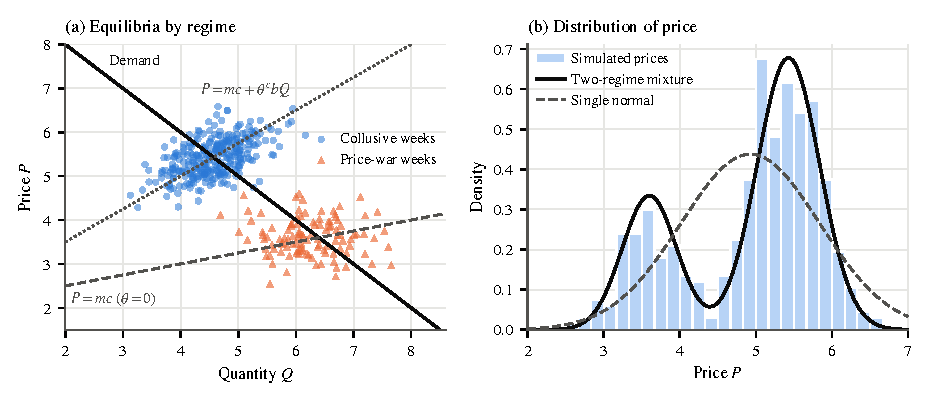
\includegraphics[width=\textwidth]{figures/ch01/regime_mixture.pdf}
\caption{Identification of conduct regimes from the distribution of the data. The simulated market has inverse demand
$P = 10 - Q + u^d$ and marginal cost $mc = 2 + 0.25\,Q + u^c$, observed for 400 weeks. Conduct is collusive
($\theta^{c} = 0.5$) with probability $\varpi = 0.7$ and competitive ($\theta^{w} = 0$) otherwise, with
$u^d \sim N(0, 0.8^2)$ and $u^c \sim N(0, 0.4^2)$. Panel (a) colors each week by its true regime, which the analyst does not observe, and draws the deterministic demand
curve and the two supply relations. Panel (b) shows the distribution of price that the analyst sees. The two-regime
mixture fits it, while a single normal distribution does not. The regime means of price, $3.6$ and $5.43$, differ by
more than four within-regime standard deviations, so the distribution is bimodal. Closer regimes could produce a single
mode. All values are illustrative.}
\label{fig:01-regimes}
\end{figure}

The main threat to this inference is that some other unobserved shock moves the supply relation. Because the
identifying variation is an error component, nothing in the procedure guarantees the conduct interpretation. Unrecorded
changes in factor prices or technology could produce the same pattern, and Porter had no factor-price data. Bresnahan
finds the conduct interpretation likely in the railroad case for two reasons. The regime shifts move price and quantity
by about 50 percent, and contemporary sources discuss cartel adherence extensively. An alternative is to fix the sample
split in advance and estimate $\theta^{c}$ and $\theta^{w}$ separately, as \citet{Bresnahan1987} does. This needs prior
information but allows a more direct check that the apparent supply shocks reflect conduct. \Cref{ch:collusion-evidence}
returns to these issues with \citet{Porter1983} and \citet{Ellison1994}.

\subsubsection{Comparative statics in industry structure}\label{sec:01-id-structure}

The fifth argument relates price to the number of firms or to concentration across similar local markets. Its logic is
familiar, but \citet[p.~1032]{Bresnahan1989} judges that it still awaited its identification arguments.
\Cref{sec:01-price-concentration} presented these studies and the six difficulties Bresnahan raises. In the language of
this section, all of them come back to the aggregate supply relation \eqref{eq:01-avg-supply}, which is
\cref{prop:01-supply-relation}(ii) applied market by market. A lower price in markets with more firms can mean lower
average conduct $\theta$ or lower average marginal cost $\overline{mc}$. Price and quantity data alone cannot apportion
the change between the two. A change in entry regulation, as in \citet{SpillerFavaro1984}, offers cleaner
variation because it moves structure for a reason unrelated to costs. The arguments of this section can then separate
the two channels, for example by checking whether demand rotations identify a lower $\theta$ after deregulation.

\subsubsection{Synthesis}\label{sec:01-id-synthesis}

\Cref{tab:01-id-strategies} summarizes the arguments. Their variety reflects the variety of data across industry
studies \citep[Section~3.6]{Bresnahan1989}. Each industry offers different information and institutional detail, and
therefore different defenses of different methods. The variety also reflects how many comparative statics of markets
with market power have no counterpart in competitive markets.

\begin{table}[htbp]
\centering
\begin{threeparttable}
\caption{How the data identify market power}
\label{tab:01-id-strategies}
\footnotesize
\setlength{\tabcolsep}{4pt}
\begin{tabularx}{\textwidth}{@{}>{\raggedright\arraybackslash}p{2.05cm}
  >{\raggedright\arraybackslash}X >{\raggedright\arraybackslash}X >{\raggedright\arraybackslash}X
  >{\raggedright\arraybackslash}p{2.2cm} >{\raggedright\arraybackslash}p{1.8cm}@{}}
\toprule
Argument & Exogenous variation & What is identified & Key maintained assumption & Applications & Full treatment \\
\midrule
Comparative statics in demand & Demand shifters that rotate demand ($Y_t$ entering $P_Q$) & Conduct $\theta$ and
  the slope of marginal cost separately & Correct demand specification; demand not of the form $\tilde P(Q, h(Y))$ &
  \citet{JustChern1980}; \citet{Bresnahan1981,Bresnahan1987} & \cref{ch:conduct} \\
\addlinespace
Homogeneity of marginal cost & Factor prices & $\theta$ from terms not multiplied by factor prices & Marginal cost
  homogeneous of degree one in observed factor prices & \citet{Appelbaum1979,Appelbaum1982} & \cref{ch:conduct} \\
\addlinespace
Comparative statics in cost & All factor prices, or taxes & Sign of $\psi$; bound on $\sum_i (1 + r_i)^{-1}$ &
  All cost shifters measured; long-run equilibrium (for $\psi$); known link to marginal cost &
  \citet{PanzarRosse1977}; \citet{Shaffer1982}; \citet{Sullivan1985}; \citet{AshenfelterSullivan1987} &
  \cref{ch:conduct} \\
\addlinespace
Direct estimation of marginal cost & Factor prices with input quantities & Marginal cost from factor demands, then
  $\theta$ & Cost-function form; correct price of capital services & \citet{GollopRoberts1979};
  \citet{Appelbaum1982}; \citet{Hall1988} & \cref{sec:01-rising-markups} \\
\addlinespace
Supply shocks & Unobserved two-valued shock to the supply relation & Frequency and size of regime changes in conduct &
  No other unobserved shifts in the supply relation & \citet{Porter1983}; \citet{LeePorter1984} &
  \cref{ch:collusion-evidence} \\
\addlinespace
Comparative statics in structure & Number of firms or concentration across local markets & Reduced-form price and
  structure relation & Structure exogenous; average cost unrelated to structure & \citet{GrahamKaplanSibley1983};
  \citet{SpillerFavaro1984} & \cref{sec:01-price-concentration} \\
\addlinespace
Residual demand & Cost shifters specific to one firm & Elasticity of the firm's residual demand & Firm's costs move
  independently of rivals' costs & \citet{BakerBresnahan1988} & \cref{ch:conduct} \\
\bottomrule
\end{tabularx}
\begin{tablenotes}\footnotesize
\item Notes: The first six rows follow the classification of \citet[Section~3]{Bresnahan1989} and are introduced in
\cref{sec:01-id-arguments}. The last row is the summary-statistic approach of his Section~4, introduced in
\cref{sec:01-neio-diffprod}. The last column gives the place in this book where each argument is developed in full.
\end{tablenotes}
\end{threeparttable}
\end{table}

\subsection{Market power with product differentiation}\label{sec:01-neio-diffprod}

Product differentiation raises short-run and long-run questions \citep[Section~4]{Bresnahan1989}. In the short run the
set of products and their attributes are fixed, and we ask how much market power existing differentiation confers. The
question has two parts. As products become more distinct, each firm's profit depends less on rivals' prices, which the
own- and cross-price elasticities of demand measure. As products become more distinct, each firm also responds less to
rivals' moves, which requires a model of competitive interaction.

The conceptual issues resemble those of the homogeneous-good case, but measurement is much harder. Suppose an industry
has $J$ products and we assume constant elasticities and symmetric cross effects. Demand still has $J$ own-price
elasticities, $J$ income elasticities and $\frac{J(J - 1)}{2}$ cross-price elasticities. With $J = 100$ products this is
\begin{equation*}
J + J + \frac{J(J - 1)}{2} = 100 + 100 + 4{,}950 = 5{,}150
\end{equation*}
elasticities, and few industries have fewer than 100 products. Multi-product firms may also have economies of scope.
Prior information from trade journals and marketing studies becomes indispensable, and how it is used varies from
industry to industry.

The most common shortcut treats the products as close substitutes, uses a price index as the observed price, and
proceeds as for a homogeneous good. Bresnahan warns that this can attribute to conduct what is due to product
differentiation \citep[p.~1046]{Bresnahan1989}. The next example makes the warning precise.

\begin{example}[Differentiation that looks like conduct]\label{ex:01-index-conduct}
Let $J$ symmetric single-product firms set prices in a Bertrand equilibrium with constant marginal cost. Let
$\varepsilon_{\mathrm{own}} > 0$ be each product's own-price elasticity (as a positive number) and
$\varepsilon_{\mathrm{cross}} \ge 0$ the cross-price elasticity between any two products. The pricing rule of
\cref{prop:01-pricing-rule} gives each firm the Lerner index $L = \frac{1}{\varepsilon_{\mathrm{own}}}$. An analyst
who treats the products as one homogeneous good measures the market elasticity when all prices move together,
\begin{equation*}
\varepsilon = \varepsilon_{\mathrm{own}} - (J - 1)\,\varepsilon_{\mathrm{cross}} ,
\end{equation*}
and reads conduct from $\frac{P - mc}{P} = \frac{\theta}{\varepsilon}$. The apparent conduct parameter is
\begin{equation*}
\tilde\theta = \varepsilon L = \frac{\varepsilon_{\mathrm{own}} - (J - 1)\,\varepsilon_{\mathrm{cross}}}{\varepsilon_{\mathrm{own}}}
 = 1 - (J - 1)\,D, \qquad D = \frac{\varepsilon_{\mathrm{cross}}}{\varepsilon_{\mathrm{own}}} .
\end{equation*}
With symmetric quantities, $D$ is the \emph{diversion ratio} between two products, the fraction of the sales lost by one
product that go to another when its price rises (\cref{ch:diffprod}). So $\tilde\theta$ is the fraction of lost sales that leave
the industry. It lies between zero and one although no firm colludes. With $J = 4$, $\varepsilon_{\mathrm{own}} = 4$ and
$\varepsilon_{\mathrm{cross}} = 1$ we get $\varepsilon = 1$, $L = 0.25$ and $\tilde\theta = 0.25$. This is exactly the
value of symmetric Cournot with four firms, produced by differentiated Bertrand competition.
\end{example}

To study differentiation directly, the analyst must reduce the dimension of the problem. Bresnahan describes three ways.

\casehead{Modeling product choice}
The first models how consumers choose among products, which yields demand systems with few parameters. Discrete-choice
models \citep[see][]{McFadden1984}, such as the nested logit, fit industries in which trade sources describe distinct
segments with much closer competition inside than across them. Spatial models of differentiation fit industries without
clear segment boundaries. In such industries, products A and B can both matter for C without A mattering for B. Spatial
models reduce the parameter count by localizing competition, and discrete-choice models do it by grouping. A
multinomial logit without nests is the limiting case in which the whole industry is one segment and competition is
symmetric. Bresnahan's spatial model of automobiles is an example \citep{Bresnahan1981,Bresnahan1987}. Any such model
is only as convincing as the information used to specify it, and the localized-versus-segmented distinction matters most.
\citet{Schmalensee1985b} proposes a test of localization based on how the prices and quantities of brands move together.
In ready-to-eat breakfast cereals he decisively rejects the model in which all brands compete equally, although he doubts
the covariance restrictions that identify the pattern of localization. \Cref{ch:discrete,ch:logit,ch:blp} develop the
modern versions of this approach.

\casehead{Aggregating products}
The second approach aggregates similar products until only a few elasticities remain. \citet{GelfandSpiller1987}
aggregate many types of bank loans into two and estimate a two-by-two system. Their model lets each bank's profit in
one market depend on rivals' strategies in both, an interdependence they write in conjectural-variations form.
\citet{Slade1987} studies ``majors'' and ``independents'' among gasoline stations in Vancouver. \citet{Suslow1986}
aggregates output into the dominant firm's product and the fringe's product. The dominant firm's marginal revenue then
depends on the substitutability of the two products, the market elasticity and the fringe supply elasticity.

\casehead{Estimating a summary statistic: residual demand}
The third approach, due to \citet{BakerBresnahan1985,BakerBresnahan1988}, estimates only the summary statistic that
measures one firm's market power. Consider the seller of product 1, facing the inverse demand
\begin{equation}\label{eq:01-bb-demand}
P_1 = P^1(Q_1, P_2, \dots, P_J, Y, \gamma),
\end{equation}
where $P_2, \dots, P_J$ are the prices of competing products. The parameter vector $\gamma$ contains the cross effects of
all $J - 1$ rivals, so it can be very long. Each rival product $j = 2, \dots, J$ has its own demand equation like
\eqref{eq:01-bb-demand} and a supply relation
\begin{equation}\label{eq:01-bb-rival}
P_j = C_q^{j}(Q_j, W_j, Z_j, \Gamma_j) - \frac{\partial P^{j}}{\partial Q_j}\, Q_j\, \vartheta_j ,
\qquad j = 2, \dots, J .
\end{equation}
These $2(J - 1)$ equations can be solved for the rivals' prices and quantities as functions of $Q_1$ and the exogenous
variables, $P_j = P_j^*(Q_1, W_{-1}, Z_{-1}, \Gamma_{-1}, \vartheta_{-1}, Y, \gamma)$. Here $W_{-1}$ and $Z_{-1}$ are the
rivals' cost shifters, and $Q_1$ remains because only the rivals' equations have been solved. Substituting into
\eqref{eq:01-bb-demand} gives the \emph{residual demand curve} of product 1,
\begin{equation}\label{eq:01-bb-residual}
P_1 = P^1\bigl(Q_1, P_2^*(\cdot), \dots, P_J^*(\cdot), Y, \gamma\bigr)
    \equiv P^{R}(Q_1, W_{-1}, Z_{-1}, \Gamma_{-1}, \vartheta_{-1}, Y, \gamma).
\end{equation}
Equations \eqref{eq:01-bb-demand} to \eqref{eq:01-bb-residual} are Bresnahan's (31), (4$^d$) and (32). By the chain rule,
the elasticity of residual inverse demand is
\begin{equation*}
-\frac{1}{\varepsilon^{R}_1} = \frac{\partial \ln P^{R}}{\partial \ln Q_1}
 = \frac{\partial \ln P^1}{\partial \ln Q_1} + \sum_{j = 2}^{J}\frac{\partial \ln P^1}{\partial \ln P_j}\,
   \frac{\partial \ln P_j^*}{\partial \ln Q_1} .
\end{equation*}
The first term is the direct effect of firm 1's output on its price. The sum adds the effect of rivals' price responses.
Substituting out the rivals' prices loses a great deal of information, since the separate elements of $\gamma$ can no
longer be estimated. That loss matters little for the question at hand. The slope of $P^{R}$ tells us how much power
firm 1 has over its price after all rivals have adjusted. Suppose product 1 is a perfect substitute for rival products
sold by price takers at constant cost. Then $P^{R}$ equals the lowest rival cost and does not respond to $Q_1$, so
$\frac{1}{\varepsilon^{R}_1} = 0$.

Residual demand can be estimated only if firm 1's costs move independently of its rivals' costs
\citep[fn.~43]{Bresnahan1989}. Its own cost shifters then serve as instruments for $Q_1$, while the rivals' cost
shifters enter \eqref{eq:01-bb-residual} directly. International markets offer natural experiments, since exchange-rate
movements change the relative costs of producers in different countries. The reciprocal
$\frac{1}{\varepsilon^{R}_1}$ of the residual-demand elasticity summarizes a firm's market power, but it does not reveal the sources of that power. It
equals the Lerner index only under particular conduct, for example when firm 1 acts as a Stackelberg leader toward
its rivals \citep[p.~289]{BakerBresnahan1988}. This is why Bresnahan leaves residual-demand studies out of his summary
table. The approach complements the
aggregation approach, which estimates every elasticity but only for a few products. \Cref{ch:conduct} treats
\citet{BakerBresnahan1988} and its application to brewing in depth.

\casehead{Market definition and policy}
These techniques bear on market definition in antitrust. Antitrust often asks whether a single firm has market power,
or whether a group of firms would have it if they acted together. \Cref{sec:01-market-definition} quoted Bresnahan's
remark that these questions are well posed even where computing shares in a relevant market is senseless. Residual
demand answers the first question directly. \citet{ScheffmanSpiller1987} extend
it to a group of firms, which answers the second. \citet{BakerBresnahan1985} ask how much steeper the residual demand of
two merging firms would be after the merger. If the two sell close substitutes and few other firms sell similar products,
each firm is an important brake on the other, and the merger steepens the curve. The Panzar-Rosse statistic gives a
related answer. A rejection of monopoly for a firm or group means that it cannot be treated as acting in isolation.
\Cref{ch:mergers} develops merger analysis with differentiated products.

\casehead{Differentiation in the long run}
In the long run firms add products, change attributes or perceptions, and new firms enter with new products or
imitations. Theory offers many strategic hypotheses: preemption by reputation for quality, preemption by filling the
product space, and coordination of product choices to soften competition. In 1989 essentially nothing empirical was known
about any of them \citep[p.~1050]{Bresnahan1989}. The same passage contains the welfare point of
\cref{sec:01-fixed-costs}. Under the Chamberlin tangency every firm prices above marginal cost, so short-run market power
says little about efficiency until we know how new products and new firms are supplied.

\subsection{What the NEIO learned}\label{sec:01-neio-lessons}

The case-study character of the NEIO raises questions of interpretation \citep[Section~5]{Bresnahan1989}. How general
are the results, and what do they reveal about market power in the economy as a whole? The SCP paradigm aimed to estimate
a map from structure to conduct and performance. Such a map would be valuable, for example to guide merger policy, which
acts on structure. A single industry study reveals at most one point on it. By 1989 NEIO studies covered more than a
dozen industries. \Cref{tab:01-bresnahan-table} reproduces the estimated Lerner indices that Bresnahan collected.

\begin{table}[htbp]
\centering
\begin{threeparttable}
\caption{Estimated Lerner indices from early NEIO studies}
\label{tab:01-bresnahan-table}
\small
\begin{tabular}{@{}llc@{}}
\toprule
Author & Industry & $L$ \\
\midrule
\citet{Lopez1984} & Food processing & 0.504 \\
\citet{Roberts1984} & Coffee roasting & 0.055 / 0.025$^{a}$ \\
\citet{Appelbaum1982} & Rubber & 0.049$^{c}$ \\
\citet{Appelbaum1982} & Textile & 0.072$^{c}$ \\
\citet{Appelbaum1982} & Electrical machinery & 0.198$^{c}$ \\
\citet{Appelbaum1982} & Tobacco & 0.648$^{c}$ \\
\citet{Porter1983} & Railroads & 0.40$^{b}$ \\
\citet{Slade1987} & Retail gasoline & 0.10 \\
\citet{Bresnahan1981} & Automobiles (1970s) & 0.1 / 0.34$^{d}$ \\
\citet{Suslow1986} & Aluminum (interwar) & 0.59 \\
\citet{SpillerFavaro1984} & Banks ``before''$^{e}$ & 0.88 / 0.21$^{f}$ \\
\citet{SpillerFavaro1984} & Banks ``after''$^{e}$ & 0.40 / 0.16$^{f}$ \\
\bottomrule
\end{tabular}
\begin{tablenotes}\footnotesize
\item Notes: $L = \frac{P - mc}{P}$. $^{a}$Largest and second-largest firm, respectively. $^{b}$When the cartel was
succeeding (0 in reversionary periods). $^{c}$At the sample midpoint. $^{d}$Varies by type of car, larger in the standard
and luxury segments. $^{e}$Uruguayan banks before and after entry deregulation. $^{f}$Large firms / small firms.
Panzar-Rosse and Sullivan studies are excluded because they yield only tests of, or bounds on, conduct.
Residual-demand studies are excluded because the reciprocal $\frac{1}{\varepsilon^{R}}$ of the residual-demand elasticity
equals the Lerner index only in special cases.
\item Source: \citet{Bresnahan1989}, Table~17.1.
\end{tablenotes}
\end{threeparttable}
\end{table}

From this evidence Bresnahan draws three guarded conclusions \citep[pp.~1052--1053]{Bresnahan1989}.

\casehead{Conclusion A}
Some concentrated industries have a great deal of market power, in the sense of high price-cost margins. Several entries
in \cref{tab:01-bresnahan-table} exceed 0.4. The industries cannot be matched systematically to census concentration
measures, because many data sets were collected by the authors. A glance at the list shows that they come overwhelmingly
from the concentrated end of the spectrum.

Two reasons warn against generalizing. First, researchers who invent a method for detecting market power apply it first
where they expect to find it. They choose concentrated industries, known or suspected cartels, or industries where earlier
case studies suggested anticompetitive conduct. Second, the data often come from trade journals, regulators or court records.
Industries with excellent trade journals are industries in which firms know a lot about their rivals, an information
structure that favors collusion. Suslow could use the trial record on Alcoa because Alcoa was suspected of market power.
More sources of data, from more industries, were needed.

\casehead{Conclusion B}
One significant cause of high margins is anticompetitive conduct. The studies separate conduct, the behavioral rules by
which firms set prices, from performance, the price-cost margin. They do not find small departures from price taking
combined with very steep demand. Several find conduct well toward the collusive end. \citet{Porter1983} and \citet{Bresnahan1987}
both find collusive conduct, although of different kinds. The railroads in Porter's study had formed the JEC by a
publicly acknowledged agreement \citep[p.~302]{Porter1983}. \citet[pp.~457 and 479]{Bresnahan1987} interprets automobile
pricing in 1954 and 1956 as tacit collusion, meaning collusive pricing without an explicit agreement among firms. His
tests compare a collusive pricing model with a Bertrand model, so they cannot reveal whether the automakers
communicated. Conduct is not uniform. \citet{Roberts1984} classifies most
coffee roasters as a price-taking fringe, while the largest firms behave less competitively without reaching the profit
maximum given the fringe.

\casehead{Conclusion C}
The new methods had taught little about the relation between market power and industry structure. The studies cover only
the concentrated end of the range, so they reveal the structure-performance map over a narrow interval. Few of them
address the causes of market power. Long-lived market power suggests that entry fails to discipline conduct, yet the
studies hardly discuss entry.

\casehead{The sources of market power}
Bresnahan closes by pointing to the causes of market power as the frontier \citep[Section~6]{Bresnahan1989}. Entry,
predation, entry deterrence and long-run strategic competition had received little empirical work with explicit
theoretical foundations. \citet{Burns1986} studies the American tobacco trust and finds that its acquisitions of
competitors became cheaper after episodes of predatory pricing. The study relies on a nineteenth-century documentary record
that modern firms would not leave. The open problem was to find the empirical implications of predation when predatory acts
must be inferred. On entry, \citet{PanzarRosse1977} add to demand and the supply relations an entry condition for the
marginal firm, $P = \mathit{LRAC}(W, Y)$, with $\mathit{LRAC}$ long-run average cost.
\citet{BresnahanReiss1990} model the entry decisions of the first two firms in a market with an integer number of firms.
They use 149 geographically isolated American markets for new car dealers. A second entrant faces nearly the same costs
and opportunities as the first, and its entry does not lower the monopoly dealer's margins by much. Both papers
argue that cross-sections of closely related markets are the right samples for studying entry. \Cref{sec:01-today-structure}
takes up the sequel by \citet{BresnahanReiss1991}.

Bresnahan's final assessment is optimistic about measurement and modest about explanation. By abandoning accounting
measures of performance, the NEIO produced a new kind of evidence of substantial market power, immune to the standard
criticisms of earlier work. Its studies are detailed enough that alternative explanations can be confronted and rebutted.
In his words, ``we know that there is market power out there, and need to know a lot more about exactly where''
\citep[p.~1055]{Bresnahan1989}. Its causes and systematic predictors remained essentially unknown.

The program that followed kept the NEIO's commitment to single industries and explicit models. Its main change was on the
demand side. Classic analyses of market power, such as \citet{Porter1983}, \citet{Bresnahan1987} and
\citet{Nevo2001}, supply the basic toolkit \citep[p.~151]{EinavLevin2010}. That toolkit combines demand and supply in
an equilibrium analysis of imperfect competition. Modern work replaces the conduct parameter with explicit models of differentiated-product
competition and estimates rich demand systems with instruments. \Cref{sec:01-today} describes this structural workflow.

\section{Empirical IO today}\label{sec:01-today}

The previous sections traced how the field moved from cross-industry regressions to studies of single
industries with explicit models of conduct. This section describes what empirical research in industrial
organization looks like after that transition. We follow the progress report of \citet{EinavLevin2010},
which maps the modern field, and we add the formal content that a survey essay leaves implicit.

Einav and Levin summarize the state of the field in a few sentences (p.~147). Most influential research
looks to economic theory for guidance, especially in modeling the behavior of firms. Studies frequently
focus on a single industry or market. They pay careful attention to institutional specifics, to the
measurement of key variables and to econometric identification. Advocates argue that, when it succeeds,
this approach combines the conceptual clarity of theory with convincing empirical measurement.

There is no recipe, but most papers share a few themes (p.~148). A study usually begins with a theory of
market equilibrium, which can be more or less explicit. The theory then plays one of three roles. It
supplies optimization or equilibrium conditions from which we infer unobserved parameters. It delivers
testable predictions. Or it helps us interpret estimated causal effects. In every case the institutional
details of the market matter, and one broad lesson from looking across industries is that they can matter
a great deal.

Industry studies have drawbacks as well (p.~147). They can lead to narrow analyses, and researchers are
often reluctant to generalize their findings to markets with different institutions. The broader lessons
therefore tend to be qualitative insights, or methods that can be applied in other settings. Critics also
argue that models resting heavily on equilibrium assumptions can obscure the link between the estimated
parameters and the variation in the data. We return to this debate in \cref{sec:01-today-debate}.

The section has six parts. \Cref{sec:01-workflow} sets out the structural workflow that organizes most of
the book. \Cref{sec:01-today-demand,sec:01-today-pricing} discuss demand estimation and the measurement of
market power. \Cref{sec:01-today-auctions} shows that auctions are pricing problems governed by the same
first-order logic. \Cref{sec:01-today-structure} turns to entry, market structure and dynamics, with a
full case study of \citet{BresnahanReiss1991}. \Cref{sec:01-today-debate} discusses the debate
between structural and design-based empirical work.

\subsection{The structural workflow: demand, supply, counterfactuals}\label{sec:01-workflow}

A large share of modern empirical IO follows a three-step workflow. We first estimate demand. We then
combine the demand estimates with a model of pricing to recover marginal costs. Finally we use the
estimated demand and costs to solve for the equilibrium under a counterfactual policy or market structure.
This subsection states the canonical model behind the workflow, derives its central equation and
illustrates the three steps. Later chapters develop each step in full.

\subsubsection{The canonical model}

Consider a market with $J$ inside products and an outside good $j = 0$. (When several markets
$t = 1, \dots, T$ appear, we add the subscript $t$.) Product $j$ has price $p_j$, a row vector of observed
characteristics $x_j$ and an unobserved demand shock $\xi_j$, which we call \emph{unobserved product
quality}. Market size is $M$, the quantity of product $j$ is $q_j$, and its market share is
$s_j = \frac{q_j}{M}$. Each firm $f$ owns a set of products $\mathcal{J}_f$, and every product has exactly
one owner.

\begin{assumption}[Canonical static model]\label{ass:01-canonical}
\leavevmode
\begin{enumerate}[label=(\roman*)]
  \item Market shares are $s_j = s_j(p, x, \xi; \gamma)$ for $j = 1, \dots, J$. Here
        $p = (p_1, \dots, p_J)^\top$ is the price vector, $x$ and $\xi$ collect the characteristics and
        demand shocks of all products, and $\gamma$ is a finite-dimensional vector of demand parameters.
        Each $s_j$ is continuously differentiable in $p$.
  \item Product $j$ has a constant marginal cost $mc_j = c(w_j, \omega_j; \Gamma)$, where $w_j$ is a vector
        of observed cost shifters, $\omega_j$ is an unobserved cost shock and $\Gamma$ is a vector of cost
        parameters. Fixed costs do not affect prices.
  \item Firms choose prices simultaneously. Each firm sets the prices of its own products to maximize their
        joint profit, taking the prices of rival products as given. We call this \emph{multi-product
        Bertrand-Nash} pricing.
  \item The equilibrium is interior, so it satisfies the first-order conditions, and the matrix
        $\Omega \odot \Delta^\top$ defined below is invertible at the equilibrium prices.
\end{enumerate}
\end{assumption}

Two matrices summarize conduct and demand. The ownership matrix $\Omega$, met with the vertical model in
\cref{sec:01-conduct-taxonomy}, is the $J \times J$ matrix with $\Omega_{jk} = 1$ if products $j$ and $k$ have the same owner and $\Omega_{jk} = 0$ otherwise. It is
symmetric and has ones on the diagonal. The matrix of share derivatives $\Delta$ has $(j, k)$ element
$\Delta_{jk} = \frac{\partial s_j}{\partial p_k}$, so row $j$ collects the effects of all prices on the
share of product $j$. The symbol $\odot$ denotes the element-wise (Hadamard) product.

\begin{proposition}[Multi-product pricing and implied marginal costs]\label{prop:01-multiproduct-foc}
Under \cref{ass:01-canonical}, equilibrium prices satisfy the system of $J$ first-order conditions
\begin{equation}\label{eq:01-foc-matrix}
  s + (\Omega \odot \Delta^\top)(p - mc) = 0,
\end{equation}
where $s$, $p$ and $mc$ are $J$-vectors. Equivalently, markups and marginal costs are
\begin{equation}\label{eq:01-implied-mc}
  p - mc = -(\Omega \odot \Delta^\top)^{-1} s,
  \qquad
  mc = p + (\Omega \odot \Delta^\top)^{-1} s .
\end{equation}
\end{proposition}

\begin{proof}
Firm $f$ earns
\[
  \pi_f = \sum_{k \in \mathcal{J}_f} (p_k - mc_k)\, M s_k(p) - C_f ,
\]
where $C_f$ is its fixed cost. Take a product $j \in \mathcal{J}_f$. The price $p_j$ enters the margin of
product $j$ and the shares of every product. By the product rule,
\[
  \frac{\partial \pi_f}{\partial p_j}
  = M s_j + M \sum_{k \in \mathcal{J}_f} (p_k - mc_k) \frac{\partial s_k}{\partial p_j} .
\]
Setting this derivative to zero and dividing by $M > 0$ gives
\[
  s_j + \sum_{k \in \mathcal{J}_f} (p_k - mc_k) \frac{\partial s_k}{\partial p_j} = 0 .
\]
The ownership matrix lets us replace the sum over the firm's products by a sum over all products:
\[
  s_j + \sum_{k = 1}^{J} \Omega_{jk} \frac{\partial s_k}{\partial p_j} (p_k - mc_k) = 0 .
\]
The derivative in this sum is $\frac{\partial s_k}{\partial p_j} = \Delta_{kj} = (\Delta^\top)_{jk}$. The
coefficient on $(p_k - mc_k)$ in the condition for product $j$ is therefore
$\Omega_{jk} (\Delta^\top)_{jk} = (\Omega \odot \Delta^\top)_{jk}$. Stacking the $J$ conditions gives
\eqref{eq:01-foc-matrix}. Premultiplying \eqref{eq:01-foc-matrix} by $(\Omega \odot \Delta^\top)^{-1}$ and
rearranging gives \eqref{eq:01-implied-mc}.
\end{proof}

The transpose has a simple origin. The condition for $p_j$ involves the effect of $p_j$ on the shares of the
firm's other products. These effects form column $j$ of $\Delta$, which is row $j$ of $\Delta^\top$.
Because $\Omega$ is symmetric, $\Omega \odot \Delta^\top = (\Omega \odot \Delta)^\top$, and some references
write the system in that form.

\begin{remark}[Special cases and conduct]\label{rem:01-foc-cases}
With single-product firms, $\Omega$ is the identity matrix. Condition $j$ then reads
$s_j + \Delta_{jj}(p_j - mc_j) = 0$, so
\[
  p_j - mc_j = -s_j\left(\frac{\partial s_j}{\partial p_j}\right)^{-1}
             = -q_j\left(\frac{\partial q_j}{\partial p_j}\right)^{-1},
\]
which is the dollar markup of \cref{prop:01-pricing-rule} applied to the residual demand $q_j$. A cartel that
maximizes the joint profit of all products sets every element of $\Omega$ equal to one. Intermediate cases
put a weight between zero and one on rival products. In this sense $\Omega$ plays the role in
differentiated-product markets that the conduct parameter $\theta$ plays in the homogeneous-good supply
relation $P = \overline{mc} - \theta P'(Q) Q$ of \cref{prop:01-supply-relation}. Equation
\eqref{eq:01-implied-mc} also shows that markups depend only on shares, share derivatives and conduct. Once
demand is known and conduct is assumed, marginal costs follow from observed prices without any cost data.
\end{remark}

\begin{example}[Same data, two conduct assumptions]\label{ex:01-two-products}
Two symmetric products sell at $p_1 = p_2 = 2$ with shares $s_1 = s_2 = 0.2$. Suppose demand estimates give
own-price derivatives $\frac{\partial s_j}{\partial p_j} = -0.4$ and cross-price derivatives
$\frac{\partial s_k}{\partial p_j} = 0.1$ (per dollar). The numbers are illustrative.

If the products have different owners, $\Omega$ is the identity and each markup is
$p_j - mc_j = \frac{0.2}{0.4} = 0.5$. Implied marginal cost is $1.5$ and the Lerner index is $0.25$.

If one firm owns both products, \eqref{eq:01-foc-matrix} becomes
\[
  \begin{pmatrix} 0.2 \\ 0.2 \end{pmatrix}
  + \begin{pmatrix} -0.4 & 0.1 \\ 0.1 & -0.4 \end{pmatrix}
    \begin{pmatrix} p_1 - mc_1 \\ p_2 - mc_2 \end{pmatrix} = 0 .
\]
By symmetry both markups equal some $m$, and each row reads $0.2 - 0.4m + 0.1m = 0$. Hence
$m = \frac{0.2}{0.3} = \frac{2}{3}$, implied marginal cost is $\frac{4}{3}$ and the Lerner index is
$\frac{1}{3}$. The diversion ratio from product 1 to product 2 (\cref{ex:01-index-conduct}), the fraction
of the sales lost by product 1 after a price increase that go to product 2, is
$D_{12} = -\frac{\partial s_2}{\partial p_1}\left(\frac{\partial s_1}{\partial p_1}\right)^{-1}
= \frac{0.1}{0.4} = \frac{1}{4}$.
In this symmetric case the joint-ownership markup equals the single-product markup divided by $1 - D_{12}$:
\[
  m = \frac{0.2}{0.4 - 0.1} = \frac{0.5}{1 - \frac{1}{4}} = \frac{2}{3} .
\]
The same prices and demand estimates thus imply different marginal costs under different conduct
assumptions. With independent cost data we could tell the two models apart. This is the logic of the
conduct tests in \cref{sec:01-today-pricing}, and diversion ratios return in \cref{ch:diffprod,ch:mergers}.
\end{example}

\subsubsection{The three steps}

\Cref{fig:01-workflow} displays the workflow. Each step uses the output of the previous one.

\begin{enumerate}[label=\textit{Step \arabic*.}, leftmargin=*, itemsep=4pt]
  \item \textit{Estimate demand.} We estimate $\gamma$ from data on shares, prices and characteristics,
        usually across many markets. Firms observe $\xi_j$ when they set prices, and
        \eqref{eq:01-implied-mc} shows that markups depend on shares. Prices are therefore correlated with
        $\xi_j$, and least squares estimates of price sensitivity are biased. The remedy is a set of
        instruments $z_j$ that satisfy $\E[\xi_j \mid z_j] = 0$ and move prices
        (\cref{sec:01-today-demand}).
  \item \textit{Recover marginal costs or test conduct.} Given $\hat\gamma$, we compute $\hat\Delta$ and the
        implied costs $\widehat{mc} = p + (\Omega \odot \hat\Delta^\top)^{-1}s$. With a cost specification
        $mc_{jt} = w_{jt}\Gamma + \omega_{jt}$, the supply-side estimating equation is
        \begin{equation}\label{eq:01-supply-eq}
          p_{jt} + \big[(\Omega_t \odot \hat\Delta_t^\top)^{-1} s_t\big]_j = w_{jt}\Gamma + \omega_{jt},
        \end{equation}
        which we estimate by least squares or instrumental variables, or jointly with demand by the
        generalized method of moments. Alternatively we compare the implied costs under several conduct
        assumptions with direct cost information.
  \item \textit{Solve for a counterfactual equilibrium.} We solve
        \begin{equation}\label{eq:01-counterfactual}
          s(p'; \hat\gamma) + \big(\Omega' \odot \Delta(p'; \hat\gamma)^\top\big)(p' - mc') = 0
        \end{equation}
        for the new price vector $p'$. A merger changes the ownership matrix to $\Omega'$. A per-unit tax
        $t$ changes costs to $mc' = \widehat{mc} + t$. A new product enlarges the choice set. The demand
        model then delivers changes in consumer welfare, and the cost estimates deliver changes in profits.
\end{enumerate}

\begin{figure}[htbp]
\centering
\begin{tikzpicture}[
  node distance=6mm and 4mm,
  box/.style={draw, rounded corners=2pt, align=flush center, text width=6.1cm, minimum height=1.05cm,
              font=\small, fill=gray!7},
  inp/.style={align=flush right, text width=2.7cm, font=\footnotesize},
  note/.style={align=flush left, text width=3.5cm, font=\footnotesize\itshape, text=black!75},
  arr/.style={-{Stealth[length=2.4mm]}, thick},
  side/.style={-{Stealth[length=1.9mm]}, semithick, black!65}
]
\node[box] (data) {\textbf{Data}\\ prices $p$, shares $s$, characteristics $x$,\\ cost shifters $w$,
  instruments $z$};
\node[box, below=of data] (dem) {\textbf{Demand model and estimation}\\ $s_j(p, x, \xi; \gamma)$
  \enspace$\Rightarrow$\enspace $\hat\gamma$, $\hat\Delta$};
\node[box, below=of dem] (foc) {\textbf{First-order conditions plus conduct}\\
  $s + (\Omega \odot \Delta^\top)(p - mc) = 0$};
\node[box, below=of foc] (mc) {\textbf{Marginal costs}\\
  $\widehat{mc} = p + (\Omega \odot \hat\Delta^\top)^{-1} s$};
\node[box, below=of mc] (cf) {\textbf{Counterfactual equilibrium}\\ solve for $p'$ under a new
  $\Omega'$, $mc'$ or choice set};
\draw[arr] (data) -- (dem);
\draw[arr] (dem) -- (foc);
\draw[arr] (foc) -- (mc);
\draw[arr] (mc) -- (cf);
\node[inp, left=of dem] (iv) {exclusion restrictions\\ $\E[\xi \mid z] = 0$};
\node[inp, left=of foc] (cond) {conduct assumption\\ (ownership $\Omega$ or $\theta$)};
\node[inp, left=of mc] (val) {cost data and\\ tests of conduct};
\node[inp, left=of cf] (pol) {policy: merger,\\ tax, new good};
\draw[side] (iv) -- (dem);
\draw[side] (cond) -- (foc);
\draw[side, dashed, {Stealth[length=1.9mm]}-{Stealth[length=1.9mm]}] (val) -- (mc);
\draw[side] (pol) -- (cf);
\node[note, right=of dem] {product space: AIDS\\ characteristic space:\\ discrete choice, logit, BLP};
\node[note, right=of foc] {multi-product pricing,\\ conduct parameters};
\node[note, right=of mc] {validation with\\ engineering or accounting costs};
\node[note, right=of cf] {mergers, new goods,\\ pass-through};
\end{tikzpicture}
\caption{The structural workflow. Solid arrows show the flow of estimates. Inputs on the left are
assumptions or outside information. Notes on the right name the models used at each step. Demand models are
developed in \cref{ch:aids,ch:discrete,ch:logit,ch:blp}, pricing and conduct in
\cref{ch:diffprod,ch:conduct}, and counterfactuals in \cref{ch:mergers,ch:newgoods}, with pass-through theory
in \cref{ch:theory}.}
\label{fig:01-workflow}
\end{figure}

The following example runs the three steps on the campus coffee shop of \cref{ex:01-coffee}. It shows that
two demand models that agree at the observed data can disagree sharply about a counterfactual.

\begin{example}[A tax on campus coffee]\label{ex:01-coffee-tax}
In \cref{ex:01-coffee} the shop charges $p = 4$ and we estimate its residual demand elasticity as
$\hat\varepsilon^R = 2.5$ with standard error $0.5$. The numbers are illustrative. If the shop sets a
monopoly price, \cref{prop:01-infer-cost} gives
\[
  \hat c = p\left(1 - \frac{1}{\hat\varepsilon^R}\right) = 4\left(1 - \frac{1}{2.5}\right) = 2.40 .
\]
Suppose the university now levies a tax of $t = 0.30$ on every coffee sold, paid by the shop. How much does
the price rise?

\emph{Pass-through in general.} With the tax, the shop maximizes $(p - c - t)Q(p)$, and its first-order
condition is
\[
  Q(p) + (p - c - t)\,Q'(p) = 0 .
\]
This condition defines the price as a function of $t$. Differentiating both sides with respect to $t$, and
writing $\rho = \frac{\dd p}{\dd t}$ for \emph{pass-through}, gives
\[
  Q'(p)\rho + (\rho - 1)\,Q'(p) + (p - c - t)\,Q''(p)\rho = 0 .
\]
Collecting the terms in $\rho$ gives
\begin{equation}\label{eq:01-passthrough}
  \rho = \frac{Q'(p)}{2Q'(p) + (p - c - t)\,Q''(p)} .
\end{equation}
Pass-through depends on the curvature $Q''$ of demand. The elasticity at the observed point does not pin
down the curvature. \Cref{ch:theory} develops this formula in full.

\emph{Constant-elasticity demand.} Let $Q(p) = A p^{-\varepsilon^R}$ with $\varepsilon^R = 2.5$. The pricing
rule is $p = \frac{\varepsilon^R}{\varepsilon^R - 1}(c + t)$, so
\[
  \rho = \frac{\varepsilon^R}{\varepsilon^R - 1} = \frac{2.5}{1.5} = \frac{5}{3} \approx 1.67 .
\]
The price rises from $\frac{5}{3} \times 2.40 = 4.00$ to $\frac{5}{3} \times 2.70 = 4.50$. The increase of
$0.50$ exceeds the tax.

\emph{Linear demand.} Let $Q(p) = A - Bp$. The monopoly price is $p = \frac{1}{2}\left(\frac{A}{B} + c\right)$.
Matching $p = 4$ with $c = 2.40$ requires $\frac{A}{B} = 5.6$. The elasticity at the observed point is then
\[
  \frac{Bp}{A - Bp} = \frac{p}{\frac{A}{B} - p} = \frac{4}{1.6} = 2.5 ,
\]
the same as before. So the two models fit the price, the elasticity and the implied marginal cost equally
well. With $Q'' = 0$, \eqref{eq:01-passthrough} gives $\rho = \frac{1}{2}$. The new price is
$\frac{1}{2}(5.6 + 2.70) = 4.15$, an increase of $0.15$.

\emph{Perfect competition.} With price-taking firms and flat marginal cost, $p = c + t$ and the price rises
by exactly $0.30$.

\emph{Sampling uncertainty.} Under constant elasticity the predicted price change is
$\frac{\varepsilon^R}{\varepsilon^R - 1}t$. Its derivative with respect to $\varepsilon^R$ is
$-\frac{t}{(\varepsilon^R - 1)^2}$. By the delta method (\cref{app:econometrics}),
\[
  \mathrm{se}(\widehat{\Delta p}) \approx \frac{t}{(\hat\varepsilon^R - 1)^2}\,\mathrm{se}(\hat\varepsilon^R)
  = \frac{0.30}{2.25} \times 0.5 \approx 0.067 .
\]
The same calculation gives $\mathrm{se}(\hat\rho) \approx \frac{0.5}{2.25} \approx 0.22$, so an approximate
95 percent confidence interval for $\rho$ is $[1.23, 2.10]$. The predicted increase ranges from $0.15$ to
$0.50$ across models, a spread far wider than the sampling error within one model. Functional form is a
substantive assumption in counterfactual work. \Cref{ch:conduct} returns to this point in the tax pass-through
test of \citet{Sumner1981} and its critiques.
\end{example}

The second step deserves a caution. Inferring marginal costs from first-order conditions is elegant and needs
no cost data, but it rests on the assumption that firms set profit-maximizing prices. Einav and Levin warn
that the approach ``can be a bit too seductive'' (p.~151). Researchers sometimes discard available cost data
because they are imperfect, even when the data could be informative or at least complementary. A few studies
combine direct and indirect cost measurement to cross-check the analysis and test the hypothesis of
equilibrium pricing. Examples are \citet{Nevo2001} for breakfast cereal (\cref{ch:blp}) and
\citet{HortacsuPuller2008} for the Texas electricity market. \Cref{ch:conduct} treats two classic
validations, \citet{GenesoveMullin1998} for sugar and \citet{Wolfram1999} for British electricity. Wolfram
measures marginal cost directly from the fuel costs and efficiencies of power plants. She finds prices above
marginal cost yet well below the predictions of Cournot and supply-function models of the two dominant
generators (p.~805). Of three explanations, regulatory constraints, the threat of entry and financial contracts,
she finds more support for the first two than for contracts (p.~806).

\subsection{Demand estimation}\label{sec:01-today-demand}

Most studies of imperfect competition begin by estimating demand. Demand is interesting in its own right
\citep[p.~148]{EinavLevin2010}. It tells us what consumers value and how they substitute between products
as prices or product offerings change. It is the input for the welfare effects of mergers and new products,
and for measuring how information or advertising affect choices. Demand elasticities are also the key input
for measuring market power, as \cref{prop:01-multiproduct-foc} shows. Many advances in this area are
econometric models that can be applied in many markets, and even outside markets.

\subsubsection{The dimensionality problem}

Einav and Levin illustrate the problem with the pricing of the iPhone (p.~148). Some consumers simply prefer
the iPhone to comparable phones, and consumers who value its interface differ from those who value a rival's
link to corporate email. Apple also sells several versions, and consumers can delay their purchase and wait
for prices to fall. Apple's pricing incentives therefore depend on a whole set of elasticities, which
describe how customers shift their purchases when Apple changes its price schedule.

A flexible demand system needs many parameters. Consider the linear system
\begin{equation}\label{eq:01-linear-system}
  q_j = a_j + \sum_{k=1}^{J} b_{jk}\, p_k + x_j \beta + \xi_j, \qquad j = 1, \dots, J,
\end{equation}
which has $J^2$ price coefficients $b_{jk}$ (p.~149). With $J = 50$ products there are 2,500 of them.
Identification requires distinct variation in each of the $J$ prices. Attractive sources of variation, such
as cost shocks, often move all prices together. Suppose, for example, that every price responds to a single
cost shifter $z$ through $p_k = \pi_k z + v_k$. Substituting into \eqref{eq:01-linear-system} gives the
reduced form
\[
  q_j = a_j + \Big(\sum_{k=1}^{J} b_{jk}\pi_k\Big) z + x_j\beta + \xi_j + \sum_{k=1}^{J} b_{jk} v_k .
\]
The shifter identifies only the combination $\sum_k b_{jk}\pi_k$ in each equation, one number for $J$
unknowns. Idiosyncratic shocks have the opposite problem: they move a few prices and leave the effects of the
others unidentified.

Demand modeling has therefore centered on a trade-off between flexible substitution patterns and the limited
variation in typical data (p.~149). There are two main strategies.

\begin{enumerate}[label=(\alph*)]
  \item \emph{Segments in product space.} We divide products into groups and restrict substitution across
        groups while allowing flexibility within them. \citet{Hausman1997} divides ready-to-eat cereals into
        adult, family and kids' segments. With $S$ equal segments of $\frac{J}{S}$ products, a linear system
        with unrestricted within-segment coefficients has $S\left(\frac{J}{S}\right)^2 = \frac{J^2}{S}$ of
        them, plus $S^2$ segment-level coefficients. For $J = 30$ and $S = 3$ this is $300 + 9$ parameters
        instead of 900. \Cref{ch:aids,ch:newgoods} develop the approach.
  \item \emph{Characteristic space.} We describe each product by a few characteristics and let consumers
        trade off price against those characteristics in a way that is common across products.
        \citet{BerryLevinsohnPakes1995} describe cars by size, horsepower and fuel efficiency, plus a quality
        characteristic $\xi_j$ that the researcher does not observe. A typical utility function is
        \begin{equation}\label{eq:01-char-utility}
          u_{ij} = x_j\beta_i - \alpha_i p_j + \xi_j + \epsilon_{ij},
        \end{equation}
        where consumer $i$ has taste coefficients $\beta_i$ and price coefficient $\alpha_i$, and
        $\epsilon_{ij}$ is an idiosyncratic shock. The number of parameters depends on the number of
        characteristics and does not grow with $J$. \Cref{ch:discrete,ch:logit,ch:blp} develop the approach.
\end{enumerate}

These techniques are the main source of the policy footprint described in \cref{sec:01-what-is-io}. They
underlie market definition and merger simulation in antitrust, damages in litigation, and the treatment of new
goods in the Consumer Price Index (\cref{ch:mergers,ch:newgoods}).

\subsubsection{Simultaneity and instruments}

Demand models are estimated from individual choice data or from aggregate prices and market shares
(p.~149). Prices respond to demand shocks, which creates a simultaneity problem. It is the imperfect
competition analogue of the textbook simultaneity of supply and demand, and researchers address it with
instrumental variables. The simplest case shows the structure. If utility \eqref{eq:01-char-utility} has
common coefficients $\beta_i = \beta$ and $\alpha_i = \alpha$, and $\epsilon_{ij}$ is type-I extreme value,
the market shares invert to the linear estimating equation
\begin{equation}\label{eq:01-logit-inversion}
  \ln s_{jt} - \ln s_{0t} = x_{jt}\beta - \alpha p_{jt} + \xi_{jt}
\end{equation}
of \citet{Berry1994}, derived in \cref{ch:logit}. Firms set higher prices for products with high $\xi_{jt}$,
so $\Cov(p_{jt}, \xi_{jt}) > 0$. Least squares then biases the estimate of $\alpha$ toward zero and makes
demand look less elastic than it is. Estimation instead uses moment conditions $\E[z_{jt}\xi_{jt}] = 0$
for instruments $z_{jt}$.

Because independent movements in many prices are rare, the most popular instruments exploit restrictions
across the equations of the demand system (pp.~149--150).

\begin{enumerate}[label=(\alph*)]
  \item \emph{Prices of the same product in other markets.} The instrument for $p_{jt}$ is, for example,
        $z_{jt} = \frac{1}{T - 1}\sum_{t' \ne t} p_{jt'}$. The idea is that, conditional on observed demand
        characteristics, prices of the same product are correlated across markets because of common costs.
        The exclusion restriction requires the demand shocks to be uncorrelated across markets,
        $\Cov(\xi_{jt}, \xi_{jt'}) = 0$ for $t \ne t'$. A national advertising campaign would violate it.
        \citet{Hausman1997} and \citet{Nevo2001} use such instruments, which we call \emph{Hausman
        instruments}.
  \item \emph{Characteristics of competing products.} The instruments are functions such as
        $\sum_{k \notin \mathcal{J}_f} x_k$ and $\sum_{k \in \mathcal{J}_f, k \ne j} x_k$, which proxy for
        the closeness of competition and so shift markups. The exclusion restriction requires that the
        characteristics be uncorrelated with $\xi$. We call these \emph{BLP instruments}.
\end{enumerate}

Neither solution is perfect, and the source of price variation and its strength must be evaluated in each
application (p.~150). Return to the iPhone. Rivals that introduce touch screens compete harder with Apple and
lead it to cut the iPhone's price, so rivals' characteristics move the iPhone's price. But suppose the rivals
were responding to the surprisingly high demand for iPhones, a high $\xi$. Then the rivals' characteristics
are correlated with $\xi$, and the exclusion restriction fails. Einav and Levin's own assessment is that many
applications are careful about the statistical conditions behind identification. They are often thin,
however, in explaining the precise source of identifying variation, in arguing why the conditions hold, and
in reporting first-stage regressions and other diagnostics (p.~150). We ask these three questions of every
demand estimate in the case studies of later chapters.

\subsubsection{Experiments and models}

Proprietary data and experiments sanctioned by firms are increasingly available (p.~150).
\citet{LewisReiley2009} analyze a large-scale experiment that randomized consumers' exposure to internet
advertising by a large retailer and then tracked their purchases. The study measures the effect of
advertising on purchases. It shows what new data technologies and cooperating firms make possible.

Experimental measurement is not a panacea, however (p.~150). An experiment measures the response to one
specific change in prices or information. A model of consumer choice links different behavioral responses to
common underlying parameters, and it translates responses into statements about welfare. Two examples
illustrate the point. \citet{HendelNevo2006} show that short-run elasticities mislead when consumers stockpile
storable goods during sales. Their model relates short-run responses to the long-run elasticities that
determine the price effects of a merger. \citet{CohenEinav2007} show how choices of insurance deductibles
reveal risk preferences under the assumption that consumers maximize expected utility. Better data will make
estimated responses more precise and more convincing, and these estimates will complement the demand models
of this book.

\subsection{Market power and pricing}\label{sec:01-today-pricing}

How far market outcomes reflect market power, or implicit or explicit collusion, is a central question of
the field. We met the three classic analyses that Einav and Levin single out (p.~151) at the end of
\cref{sec:01-neio-lessons}. They are \citet{Porter1983} on the railroad cartel of the 1880s,
\citet{Bresnahan1987} on the automobile industry and \citet{Nevo2001} on breakfast cereal. The first two estimate conduct in the
NEIO manner. The third shows the modern form of the toolkit.

Underlying each study is a model of market equilibrium. The most common one is Bertrand-Nash price
competition with differentiated products. In equilibrium each firm sets price equal to marginal cost plus a
markup that depends on the semi-elasticity of its demand, taking rivals' prices as given. This is
\cref{prop:01-multiproduct-foc}. With estimates of demand and costs, these conditions let us compute
equilibrium prices. They also let us test noncooperative pricing against alternatives such as collusion.
Because accounting data rarely measure economic marginal cost (\cref{sec:01-what-is-io}), a typical study
estimates demand, computes the optimal markup and subtracts it from the observed price, as \citet{Rosse1970}
did. This is Step~2 of the workflow.

\subsubsection{Testing conduct}

The same logic turns conduct into a testable hypothesis. Let $m = 1, \dots, \bar m$ index a menu of conduct
models, each with its own matrix $\Omega^m$. Examples are single-product pricing, pricing by the actual
multi-product owners and joint profit maximization. Model $m$ implies the markup vector
$b^m = -(\Omega^m \odot \hat\Delta^\top)^{-1}s$ and the cost vector $mc^m = p - b^m$. There are two ways
to confront the menu with data. The first compares the implied margins with direct measures of cost or margin.
\citet{Nevo2001} compares the margins implied by the three models above with accounting margins in the cereal
industry. The second specifies costs as $mc_{jt} = w_{jt}\Gamma + \omega_{jt}$ and writes, for each model,
\begin{equation}\label{eq:01-conduct-test}
  p_{jt} - b^m_{jt}(\hat\gamma) = w_{jt}\Gamma + \omega^m_{jt}, \qquad \E\big[\omega^m_{jt} \mid z_{jt}\big] = 0
  \text{ under model } m .
\end{equation}
Only the true model satisfies the moment condition. Instruments that move markups differently across
models, such as changes in rivals' products or in ownership, give the comparison power. \citet{Bresnahan1987}
uses non-nested (Cox) tests to compare collusive and competitive models of automobile pricing in 1954, 1955
and 1956 (\cref{ch:discrete}). The homogeneous-good version, with the conduct parameter $\theta$, is the
subject of \cref{ch:conduct}.

\subsubsection{Beyond traditional product markets}

The basic framework supports a wide range of analyses (p.~151). Early industry studies focused on
distinguishing unilateral market power from collusion and on the price and welfare effects of mergers, taxes
and new goods. Later work added search costs, price discrimination, retail sales, consumer stockpiling,
adverse selection and nonprice strategies for attracting customers. Einav and Levin give three examples
(p.~152).
\begin{itemize}
  \item \citet{EllisonEllison2009} study how an internet price comparison engine affects competition among
        online retailers. Carefully documented price variation shows that the engine's price ranking makes
        consumers extremely price sensitive. Retailers then have an incentive to \emph{obfuscate}, that is,
        to manipulate consumer search so as to soften otherwise cut-throat price competition.
  \item \citet{GentzkowShapiro2010} construct a measure of newspaper ``slant'' and estimate consumer demand
        for slant from variation in the distribution areas of local newspapers. They use the estimated demand
        in a model of the slant chosen by newspaper owners.
  \item \citet{EinavJenkinsLevin2012} use discrete shifts in pricing to estimate the demand for subprime auto
        loans. They embed the estimates in a model of loan pricing to study screening and credit terms set
        by a lender with market power.
\end{itemize}
Detailed data and transparent identification matter in these studies. Yet their results are most interesting
through the lens of a theoretical model (p.~152). Any empirical result applies to one setting at one time,
and markets differ a great deal. What makes these studies meaningful beyond their setting is that they
illuminate mechanisms. Manipulation of consumer search, catering to ideological preferences and pricing under
asymmetric information also operate in other markets.

The same methods changed antitrust practice, which moved from concentration ratios and Herfindahl-Hirschman
indices to econometric studies of the industry under review (\cref{sec:01-what-is-io}). The Department of
Justice and the Federal Trade Commission use such studies to define markets and to assess the likely price
effects of a merger or the risk of collusion. These exercises draw on academic research and in turn motivate
new empirical models (p.~152 and \cref{ch:mergers}).

\subsection{Auctions as pricing problems}\label{sec:01-today-auctions}

Many intermediate goods are traded in \emph{bidding markets}. Firms and governments solicit bids to procure
goods and services, and they use auctions to sell resources in limited supply. The connection between bidding
markets and price competition is very close, although it is not always appreciated
\citep[pp.~152--153]{EinavLevin2010}. Empirical methods for auctions parallel the framework of the previous
subsections \citep{AtheyHaile2006,HendricksPorter2007}. A bidder trades off a higher probability of winning
against a higher margin if she wins. A firm posting a price trades off higher sales against a higher margin.
The next proposition makes the parallel exact.

\begin{assumption}[Single-agent pricing problems]\label{ass:01-auction-basic}
\leavevmode
\begin{enumerate}[label=(\roman*)]
  \item Agents are risk neutral. Each bidder knows her own cost or value, and the costs or values of
        different bidders are independent (independent private values).
  \item Each agent takes as given the demand curve or the distribution of rival bids that she faces. In a
        Bayesian Nash equilibrium this distribution is the one induced by the rivals' bidding strategies.
  \item The relevant distribution functions are differentiable with positive densities, ties occur with
        probability zero, and the optimum is interior.
\end{enumerate}
\end{assumption}

\begin{proposition}[One markup rule for prices and bids]\label{prop:01-unified-markup}
Under \cref{ass:01-auction-basic}:
\begin{enumerate}[label=(\roman*)]
  \item A firm with constant marginal cost $c$ facing residual demand $Q(p)$, with $Q' < 0$, maximizes
        $(p - c)Q(p)$. Its optimal price satisfies
        \begin{equation}\label{eq:01-unified-price}
          p = c - \frac{Q(p)}{Q'(p)} .
        \end{equation}
  \item In a procurement auction won by the lowest of $N$ bids, a bidder with cost $c$ faces $N - 1$ rivals
        whose bids are independent draws from a distribution $G$ with density $g$. She wins with
        probability $\big(1 - G(b)\big)^{N-1}$, maximizes $(b - c)\big(1 - G(b)\big)^{N-1}$, and her optimal bid
        satisfies
        \begin{equation}\label{eq:01-unified-procurement}
          b = c + \frac{1 - G(b)}{(N - 1)\,g(b)} .
        \end{equation}
  \item In a first-price sale auction with $N$ bidders, a bidder with value $v$ faces $N - 1$ rivals whose
        bids are independent draws from a distribution $G$ with density $g$. She wins with probability
        $G(b)^{N-1}$, maximizes $(v - b)G(b)^{N-1}$, and her optimal bid satisfies
        \begin{equation}\label{eq:01-unified-sale}
          v = b + \frac{G(b)}{(N - 1)\,g(b)} .
        \end{equation}
\end{enumerate}
In each case the margin equals the reciprocal of the semi-elasticity of the probability of trade (or of
quantity) with respect to the agent's own price.
\end{proposition}

\begin{proof}
(i) The first-order condition is $Q(p) + (p - c)Q'(p) = 0$. Dividing by $-Q'(p) > 0$ gives
$p - c = -\frac{Q(p)}{Q'(p)}$, which is \eqref{eq:01-unified-price} and \cref{prop:01-pricing-rule}.

(ii) Differentiating $(b - c)\big(1 - G(b)\big)^{N-1}$ with respect to $b$ and setting the result to zero gives
\[
  \big(1 - G(b)\big)^{N-1} - (b - c)(N - 1)\big(1 - G(b)\big)^{N-2} g(b) = 0 .
\]
Dividing by $(N - 1)\big(1 - G(b)\big)^{N-2}g(b) > 0$ gives $b - c = \frac{1 - G(b)}{(N - 1)g(b)}$, which is
\eqref{eq:01-unified-procurement}.

(iii) Differentiating $(v - b)G(b)^{N-1}$ with respect to $b$ and setting the result to zero gives
\[
  -G(b)^{N-1} + (v - b)(N - 1)\,G(b)^{N-2} g(b) = 0 .
\]
Dividing by $(N - 1)G(b)^{N-2}g(b) > 0$ gives $v - b = \frac{G(b)}{(N - 1)g(b)}$, which is
\eqref{eq:01-unified-sale}.

For the last claim, let $D(x)$ be the quantity sold or the probability of trade at the agent's price $x$. A
seller maximizes $(x - c)D(x)$ with $D' < 0$, and the first-order condition gives
$x - c = -\frac{D(x)}{D'(x)} = \left\lvert \frac{\dd \ln D(x)}{\dd x} \right\rvert^{-1}$. In case (i),
$D = Q$. In case (ii), $D = (1 - G)^{N-1}$, so $-\frac{D'}{D} = \frac{(N - 1)g}{1 - G}$. A buyer maximizes $(v - x)D(x)$ with $D' > 0$, and
the first-order condition gives $v - x = \frac{D(x)}{D'(x)} = \left(\frac{\dd \ln D(x)}{\dd x}\right)^{-1}$.
In case (iii),
$D = G^{N-1}$, so $\frac{D'}{D} = \frac{(N - 1)g}{G}$.
\end{proof}

\Cref{tab:01-unified} lines up the three problems. Rules (ii) and (iii) are mirror images of each other.
Einav and Levin state the procurement rule and rule (i) side by side in their footnote 3 (p.~153). Their $G$
is the distribution of the lowest rival bid, which we write $G_{\min}$. All $N - 1$ rivals bid above $b$
exactly when the lowest rival bid does, so $1 - G_{\min}(b) = \big(1 - G(b)\big)^{N-1}$. Rule (ii) then reads
$b = c + \frac{1 - G_{\min}(b)}{g_{\min}(b)}$, their form. In the same way, rule (iii) reads
$v = b + \frac{G_{\max}(b)}{g_{\max}(b)}$, where $G_{\max}(b) = G(b)^{N-1}$ is the distribution of the
highest rival bid. The proposition describes a single bidder's best response. That the first-order condition
characterizes equilibrium bidding when every bidder uses an increasing strategy is shown in
\cref{ch:auction-theory}.

\begin{table}[htbp]
\centering
\caption{Posted prices and auctions as one pricing problem}
\label{tab:01-unified}
\footnotesize
\begin{tabularx}{\textwidth}{@{}>{\raggedright\arraybackslash}p{2.35cm}
  >{\raggedright\arraybackslash}X >{\raggedright\arraybackslash}X >{\raggedright\arraybackslash}X@{}}
\toprule
 & Posted price & Procurement auction & First-price sale auction \\
\midrule
Choice & price $p$ & bid $b$ & bid $b$ \\
Objective & $(p - c)Q(p)$ & $(b - c)\big(1 - G(b)\big)^{N-1}$ & $(v - b)G(b)^{N-1}$ \\
``Demand'' faced & residual demand $Q(p)$ & probability $\big(1 - G(b)\big)^{N-1}$ that all rivals bid more &
  probability $G(b)^{N-1}$ that all rivals bid less \\
Inversion & $c = p + \frac{Q(p)}{Q'(p)}$ & $c = b - \frac{1 - G(b)}{(N - 1)g(b)}$ &
  $v = b + \frac{G(b)}{(N - 1)g(b)}$ \\
What we estimate & demand system, with instruments for price & distribution of bids &
  distribution of bids \\
Main confounder & demand shocks $\xi$ correlated with price & unobserved auction heterogeneity &
  unobserved auction heterogeneity \\
Origin & \citet{Rosse1970} & \citet{GuerrePerrigneVuong2000} & \citet{GuerrePerrigneVuong2000} \\
\bottomrule
\end{tabularx}
\par\smallskip
\begin{minipage}{\textwidth}\footnotesize
\textit{Notes:} $c$ is marginal cost, $v$ is the bidder's value, $G$ and $g$ are the distribution function
and density of each rival's bid, and $N$ is the number of bidders. Each inversion follows from
\cref{prop:01-unified-markup}.
\end{minipage}
\end{table}

\subsubsection{From bids to values}

The proposition is the basis of the estimator of \citet{GuerrePerrigneVuong2000}. Rosse inferred costs from
prices. In the same way, we can infer values or costs from bids (p.~153). In a posted-price market, the
inversion $\hat c = p + \frac{Q(p)}{\hat Q'(p)}$ requires an estimate of demand, which in turn requires
instruments. In a first-price auction the object playing the role of demand is the distribution of rival bids.
That distribution is observed directly: every bid in a sample of comparable auctions is a draw from $G$. The
estimator has two steps.
\begin{enumerate}[label=(\arabic*)]
  \item Estimate $G$ and $g$ from the pooled bids of auctions with the same number of bidders and similar
        observed characteristics, for example by kernel methods.
  \item Compute a \emph{pseudo-value} for each bid,
        \begin{equation}\label{eq:01-pseudo-values}
          \hat v_i = b_i + \frac{\hat G(b_i)}{(N - 1)\,\hat g(b_i)},
        \end{equation}
        and estimate the distribution of values from the pseudo-values.
\end{enumerate}
No instrument is needed because, under independent private values and symmetric equilibrium, the bids that
generate $G$ are the bids we observe. The analogue of the demand shock $\xi$ is \emph{unobserved auction
heterogeneity}, a feature of the object that bidders see and the researcher does not. It shifts all bids in an
auction together and breaks the simple inversion. \Cref{ch:auction-empirics} treats it, including the
deconvolution approach of \citet{Krasnokutskaya2011}.

\begin{example}[The inversion with uniform values]\label{ex:01-gpv-uniform}
Let values be independent and uniform on $[0, 1]$ with $N$ bidders. The symmetric equilibrium of the
first-price auction, derived in \cref{ch:auction-theory}, is $b(v) = \frac{N - 1}{N}v$. Bids are then uniform
on $\left[0, \frac{N - 1}{N}\right]$, so
\[
  G(b) = \frac{N b}{N - 1}, \qquad g(b) = \frac{N}{N - 1} .
\]
Substituting into \eqref{eq:01-unified-sale} gives
\[
  b + \frac{G(b)}{(N - 1)g(b)}
  = b + \frac{\frac{Nb}{N - 1}}{(N - 1)\frac{N}{N - 1}}
  = b + \frac{b}{N - 1}
  = \frac{N}{N - 1}\, b = v .
\]
The inversion recovers the value exactly. The bidder's margin is $v - b = \frac{v}{N}$, which falls as the
number of bidders grows. It mirrors the Cournot Lerner index $\frac{1}{N\varepsilon}$ of
\cref{prop:01-cowling-waterson}.
\end{example}

\subsubsection{Applications}

Auctions also offer a laboratory for strategic behavior under asymmetric information. Einav and Levin
describe four lines of work (pp.~153--154), which later chapters develop.
\begin{itemize}
  \item \citet{AtheyLevinSeira2011} study U.S. Forest Service timber sales. In the 1980s the Forest Service
        used both sealed-bid and open ascending auctions, in some cases choosing the format at random.
        Regressions exploiting this variation show that sealed-bid auctions attract more small bidders,
        shift the allocation toward them and can raise revenue. A private-value model with endogenous
        participation and bidders of different sizes and technologies matches these patterns. The authors use
        the estimated model to assess bidder competitiveness, including the possibility of collusion in some
        auctions. Theory translates bids into values that support predictions out of sample, and the
        variation in format provides a sharp test (p.~154). The paper is a deep dive in
        \cref{ch:auction-empirics}.
  \item \citet{HendricksPorter1988} study federal auctions of offshore oil leases on the Outer Continental
        Shelf. They focus on sales from 1959 to 1969 of ``drainage'' tracts, which lie next to tracts where
        deposits have been found. The owner of the neighboring lease has extra information about a
        drainage tract, whereas newly opened ``wildcat'' tracts favor no bidder. The
        outcomes differ sharply across the two cases, and the better-informed neighbors earn profits in the
        way the theory of asymmetric information predicts. With the later work of
        \citet{HendricksPinksePorter2003}, this study provides some of the sharpest evidence for equilibrium
        models of asymmetric information.
  \item Search advertising auctions combine auction methods with large data sets and field experiments.
        \citet{Varian2009} infers advertisers' values from Google data under optimal bidding and estimates the
        division of surplus. \citet{OstrovskySchwarz2009} use a calibrated model of equilibrium bidding to
        derive optimal reserve prices for Yahoo!'s sponsored search auctions. They implement the reserve
        prices in a large field experiment and track the resulting increase in revenue. Theory makes
        predictions ``before the fact'' or ``outside the data'' (p.~154).
  \item In restructured wholesale electricity markets, generators bid to supply power.
        \citet{BorensteinBushnellWolak2002} analyze the California market. They argue that the price spike
        of the summer of 2000 was due in large part to the exercise of market power, rather than to higher
        production costs.
\end{itemize}

\subsection{Market structure and dynamics}\label{sec:01-today-structure}

A classic question dates back at least to Bain's work in the 1950s \citep[p.~154]{EinavLevin2010}. It asks how
the set of firms in an industry and their capabilities affect competition, innovation and other outcomes. It
leads to a second question: what determines the set of firms, and which barriers to entry keep markets
imperfectly competitive? Entry, market structure and dynamics lie outside the main scope of this edition.
We nevertheless treat the entry model of \citet{BresnahanReiss1991} in some detail. It gives a clean modern
answer to the question that the SCP regressions of \cref{sec:01-scp} tried to answer.

\subsubsection{Entry events}

One approach studies specific episodes of entry or exit (pp.~154--155). \citet{GoolsbeeSyverson2008} study how
incumbent airlines respond when Southwest Airlines threatens to enter a route. Fares fall sharply, and the
decline begins before Southwest enters. It starts once Southwest operates at both endpoints of the route, which
makes entry probable. We cite the working-paper version (NBER Working Paper 11072, revised August 2008).
According to its abstract, over half of Southwest's total effect on incumbent fares occurs before Southwest
starts flying the route (\cref{ch:airlines} treats airline entry).
\citet{EllisonEllison2011} test for strategic entry deterrence by pharmaceutical incumbents just before their
patents expire. Their test exploits variation in market size. Deterrence is unnecessary in very small markets,
which attract no entrants, and impossible in very large ones, which attract entrants anyway. Strategic
investment can therefore be nonmonotone in market size, whereas investment without a deterrence motive is
monotone under their conditions. The working-paper version (NBER Working Paper 13069, 2007) studies drugs
that lost patent protection between 1986 and 1992. In it, incumbents in markets of intermediate size advertise
less and are more likely to cut advertising just before expiry.

\subsubsection{Entry thresholds: theory}

A second approach, pioneered by \citet{BresnahanReiss1991}, also relies on variation in market size. It adds
the assumption that markets are in long-run equilibrium (p.~155). The idea, which also appears in
\citet{Sutton1991}, is that variable profits scale with the size of the market while fixed costs do not.

\begin{assumption}[Entry with market-size scaling]\label{ass:01-br}
\leavevmode
\begin{enumerate}[label=(\roman*)]
  \item Market demand is $Q = M\,d(p, X)$, where $M$ is the number of consumers, $d$ is the demand of a
        representative consumer and $X$ shifts it. Doubling $M$ doubles demand at every price.
  \item The $N$ active firms are symmetric. In the post-entry equilibrium they charge $p_N$ and share demand
        equally. Industry variable profit per consumer, $v_N = \big(p_N - AVC\big)\,d(p_N, X)$, depends on
        $N$ but not on $M$, where $AVC$ is average variable cost.
  \item Every firm pays the same fixed cost $F > 0$.
  \item Entry does not raise industry variable profit per consumer, which stays positive:
        $0 < v_{N+1} \le v_N$ for all $N$.
  \item Entry is free. Firms enter as long as an entrant earns nonnegative profit.
\end{enumerate}
\end{assumption}

Under these assumptions each of $N$ firms earns
\begin{equation}\label{eq:01-br-profit}
  \Pi_N(M) = \frac{M}{N}\,v_N - F .
\end{equation}
We define the \emph{entry threshold} $M_N^*$ as the market size at which $N$ firms just break even, and the
\emph{per-firm threshold} $\tau_N = \frac{M_N^*}{N}$ as the number of consumers each firm needs.

\begin{proposition}[Entry thresholds]\label{prop:01-entry-thresholds}
Under \cref{ass:01-br}:
\begin{enumerate}[label=(\roman*)]
  \item $N$ firms break even if and only if $M \ge M_N^*$, where $M_N^* = \frac{N F}{v_N}$.
  \item The thresholds are strictly increasing: $M_1^* < M_2^* < M_3^* < \cdots$.
  \item The free-entry number of firms is the unique $N^*$ with $\Pi_{N^*}(M) \ge 0 > \Pi_{N^* + 1}(M)$.
        Equivalently, $N^* = N$ if and only if $M_N^* \le M < M_{N+1}^*$, and $N^* = 0$ if $M < M_1^*$.
  \item The per-firm threshold is $\tau_N = \frac{F}{v_N}$, and the \emph{entry threshold ratio} is
        \begin{equation}\label{eq:01-etr}
          \frac{\tau_{N+1}}{\tau_N} = \frac{v_N}{v_{N+1}} \ge 1 ,
        \end{equation}
        with equality if and only if the entry of firm $N + 1$ leaves variable profit per consumer unchanged.
\end{enumerate}
\end{proposition}

\begin{proof}
(i) From \eqref{eq:01-br-profit}, $\Pi_N(M) \ge 0$ if and only if $\frac{M v_N}{N} \ge F$. Multiplying by
$\frac{N}{v_N} > 0$ gives $M \ge \frac{N F}{v_N} = M_N^*$.

(ii) Because $v_{N+1} \le v_N$,
\[
  M_{N+1}^* = \frac{(N + 1)F}{v_{N+1}} \ge \frac{(N + 1)F}{v_N} > \frac{N F}{v_N} = M_N^* .
\]

(iii) With $N$ firms in the market, free entry requires two conditions. Incumbents must not lose money, so
$\Pi_N(M) \ge 0$. A further entrant must lose money, so $\Pi_{N+1}(M) < 0$. By part (i) the two conditions
are $M \ge M_N^*$ and $M < M_{N+1}^*$. By part (ii) the intervals $[M_N^*, M_{N+1}^*)$ are disjoint and
cover $[M_1^*, \infty)$, so exactly one $N$ satisfies both. If $M < M_1^*$, a monopolist loses money and no
firm enters.

(iv) Dividing $M_N^*$ by $N$ gives $\tau_N = \frac{F}{v_N}$. Taking the ratio for $N + 1$ and $N$ gives
$\frac{\tau_{N+1}}{\tau_N} = \frac{v_N}{v_{N+1}}$, which is at least one by \cref{ass:01-br}(iv) and equals
one exactly when $v_{N+1} = v_N$.
\end{proof}

The ratio in \eqref{eq:01-etr} measures how competition changes as firms enter. Suppose it takes 800 residents
to support one dentist, the illustration of Einav and Levin (p.~155). If a second dentist neither lowers
margins nor changes entry costs, a town of 1,600 can support two dentists. If the second dentist intensifies
competition, two dentists need more than 1,600 residents. Einav and Levin state the model in their footnote
4 as $\pi(n) = S\,q(p_n)(p_n - c)$ and $\pi(n) > F > \pi(n + 1)$, where $S$ is market size and $q(p)$ is
``the share of potential customers who purchase.'' In our notation $S = M$. Because $\pi(n)$ is the profit of
one firm, we read $q(p_n)$ as the share of potential customers who buy from a given firm. This reading is ours,
and with it $\pi(n) = \frac{M}{n}v_n$.

\begin{remark}[What the ratio does and does not reveal]\label{rem:01-etr-meaning}
The ratio measures the change in conduct as $N$ grows. It says nothing about the level of conduct. A perfect
cartel earns the monopoly variable profit per consumer whatever the number of members, so $v_N$ is constant
and every ratio equals one. Perfect competition among firms with U-shaped average costs also gives ratios of
one, because each firm needs enough customers to produce at minimum efficient scale. At the other extreme,
homogeneous Bertrand competition with constant marginal cost gives $v_N = 0$ for $N \ge 2$, so no duopoly
ever forms. This case lies outside \cref{ass:01-br}(iv), which requires $v_N > 0$. We read its thresholds as
$M_N^* = \infty$ for $N \ge 2$. A ratio near one after a few entrants is therefore consistent with competition or with collusion.
Bresnahan and Reiss acknowledge that without price or quantity data they cannot tell the two apart (working
paper, p.~8, fn.~8).
\end{remark}

\begin{remark}[Heterogeneous entrants]\label{rem:01-etr-costs}
Let later entrants pay higher fixed costs $F_N$, because they are less efficient or face entry barriers.
Repeating the proof gives $\tau_N = \frac{F_N}{v_N}$ and
\[
  \frac{\tau_{N+1}}{\tau_N} = \frac{F_{N+1}}{F_N}\cdot\frac{v_N}{v_{N+1}} .
\]
A ratio above one can then reflect costlier entrants as well as tougher competition. Other departures shift the
ratios too. A monopolist that price discriminates earns more per customer, which lowers $\tau_1$ and raises
$\frac{\tau_2}{\tau_1}$. Product differentiation softens competition and lowers $\tau_N$ relative to $\tau_1$.
Separating these channels requires maintained assumptions about costs.
\end{remark}

\begin{example}[Entry thresholds under Cournot competition]\label{ex:01-cournot-thresholds}
Let per-capita demand be $d(p) = \frac{a - p}{b}$, so market inverse demand is $p = a - b\frac{Q}{M}$. Firms
have constant marginal cost $c < a$ and compete in quantities. Firm $i$ maximizes
$\left(a - b\frac{Q}{M} - c\right)q_i$, with first-order condition
\[
  a - b\frac{Q}{M} - c - b\frac{q_i}{M} = 0 .
\]
In the symmetric equilibrium $q_i = \frac{Q}{N}$. Substituting and solving gives
\[
  Q = \frac{M N (a - c)}{b(N + 1)}, \qquad p_N = \frac{a + Nc}{N + 1}, \qquad p_N - c = \frac{a - c}{N + 1} .
\]
Per-capita demand is $d(p_N) = \frac{Q}{M} = \frac{N(a - c)}{b(N + 1)}$, so
\[
  v_N = (p_N - c)\,d(p_N) = \frac{N(a - c)^2}{b(N + 1)^2} .
\]
\Cref{prop:01-entry-thresholds} then gives
\[
  M_N^* = \frac{N F}{v_N} = \frac{F b (N + 1)^2}{(a - c)^2},
  \qquad
  \frac{\tau_{N+1}}{\tau_N} = \frac{v_N}{v_{N+1}} = \frac{N(N + 2)^2}{(N + 1)^3} .
\]
The ratios are $\frac{9}{8} = 1.125$ for the second firm, $\frac{32}{27} \approx 1.185$ for the third,
$\frac{75}{64} \approx 1.172$ for the fourth and $\frac{144}{125} = 1.152$ for the fifth, and they tend to one
as $N$ grows. A duopoly needs $\frac{9}{4}$ times the market of a monopoly. \Cref{fig:01-thresholds} plots the
profit lines. Linear Cournot competition thus implies a gradual decline in margins, with ratios a little above
one for every entrant.
\end{example}

\begin{figure}[htbp]
\centering
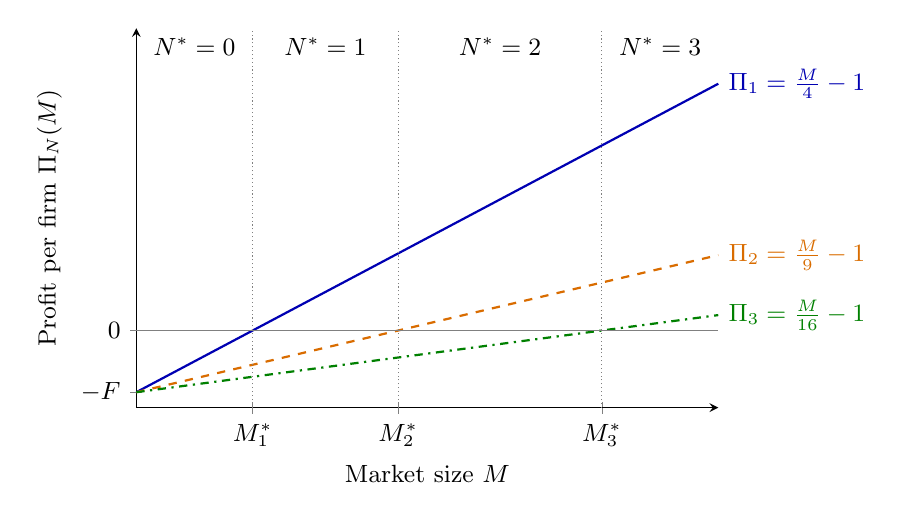
\begin{tikzpicture}
\begin{axis}[
  width=0.74\textwidth, height=6.4cm,
  xmin=0, xmax=20, ymin=-1.25, ymax=4.9,
  axis lines=left,
  clip=false,
  xlabel={Market size $M$}, ylabel={Profit per firm $\Pi_N(M)$},
  xtick={4,9,16}, xticklabels={$M_1^*$, $M_2^*$, $M_3^*$},
  ytick={-1,0}, yticklabels={$-F$, $0$},
  every axis plot/.append style={thick},
  label style={font=\small}, tick label style={font=\small}
]
\addplot[domain=0:20, samples=2, blue!70!black] {x/4 - 1}
  node[pos=1, right, font=\small] {$\Pi_1 = \frac{M}{4} - 1$};
\addplot[domain=0:20, samples=2, orange!85!black, dashed] {x/9 - 1}
  node[pos=1, right, font=\small] {$\Pi_2 = \frac{M}{9} - 1$};
\addplot[domain=0:20, samples=2, green!50!black, dash dot] {x/16 - 1}
  node[pos=1, right, font=\small] {$\Pi_3 = \frac{M}{16} - 1$};
\draw[gray, thin] (axis cs:0,0) -- (axis cs:20,0);
\draw[gray, densely dotted] (axis cs:4,-1.25) -- (axis cs:4,4.9);
\draw[gray, densely dotted] (axis cs:9,-1.25) -- (axis cs:9,4.9);
\draw[gray, densely dotted] (axis cs:16,-1.25) -- (axis cs:16,4.9);
\node[font=\small] at (axis cs:2,4.6) {$N^* = 0$};
\node[font=\small] at (axis cs:6.5,4.6) {$N^* = 1$};
\node[font=\small] at (axis cs:12.5,4.6) {$N^* = 2$};
\node[font=\small] at (axis cs:18,4.6) {$N^* = 3$};
\end{axis}
\end{tikzpicture}
\caption{Entry thresholds under linear Cournot competition (\cref{ex:01-cournot-thresholds}) with the
normalization $\frac{(a - c)^2}{b} = 1$ and $F = 1$. Profit per firm is $\Pi_N = \frac{M}{(N + 1)^2} - 1$.
Each line crosses zero at the threshold $M_N^* = (N + 1)^2$, and the bands show the free-entry number of
firms $N^*$.}
\label{fig:01-thresholds}
\end{figure}

\subsubsection{Bresnahan and Reiss (1991): entry into isolated markets}

\casehead{Question}
How much does entry change competition in a concentrated market? Theories give conflicting answers.
Contestability says that the threat of entry alone disciplines incumbents, while many entry-barrier theories
say that only actual entry matters. \citet{BresnahanReiss1991} propose to measure the effect of each
additional entrant from the relation between market size and the number of firms. The numbers below come
from the working-paper version of the article (Stanford GSB Research Paper 1061).

\casehead{Setting and data}
The sample consists of 202 geographically isolated local markets in the United States.
The typical market is a county seat in the western United States, and the population of the central town
approximates market size. The towns lie at least 25 miles from the nearest town of 1,000 people or more, and
towns within 100 miles of a city of 100,000 are excluded.
Isolation makes it easy to count all competitors. The authors keep only industries whose sellers offer a
narrowly defined product or service and can all be identified. Five survive their data requirements:
doctors, dentists, druggists, plumbers and tire dealers. Firms are counted from telephone books and trade
sources and checked by visits. Practices that share an address and a telephone number count as one firm. In
the sample, mean town population is 3,740, ranging from 120 to 45,090, and the mean number of dentists is
2.6 (working paper, Table~2).
Of the 202 markets, 32 have no dentist, 67 have one and 39 have two (Table~1).

\casehead{Model and estimating equations}
The empirical model generalizes \eqref{eq:01-br-profit} by letting market size, variable profit and fixed
costs depend on observables. The parameter names below are ours, because the paper's symbols clash with the
notation of this book. In market $t$ the profit of each of $N$ firms is
\begin{equation}\label{eq:01-br-latent}
  \Pi_{Nt} = M_t(\lambda)\,V_N(X_t) - F_N(W_t) + u_t .
\end{equation}
The profit shock $u_t$ is standard normal and independent across markets and of the observables. It is common
to all firms in a market. Market size is
\[
  M_t(\lambda) = \mathit{TownPop}_t + \lambda_1 \mathit{NearbyPop}_t + \lambda_2 \mathit{PosGrowth}_t
  + \lambda_3 \mathit{NegGrowth}_t + \lambda_4 \mathit{Commuters}_t ,
\]
with the coefficient on town population normalized to one. The other terms are population within ten miles,
the positive and negative parts of town growth between 1970 and 1980, and residents who commute to work outside
the county. Per-firm variable profit per consumer and fixed costs are
\[
  V_N(X_t) = \eta_1 + X_t\beta^V - \sum_{n=2}^{N}\eta_n ,
  \qquad
  F_N(W_t) = \zeta_1 + \zeta_L W_{Lt} + \sum_{n=2}^{N}\zeta_n ,
\]
The vector $X_t$ contains county demographics such as per capita income. The variable $W_{Lt}$ is the value of
farmland, a proxy for the cost of capital. The parameter $\eta_n$ measures the fall in each firm's variable profit per
consumer when the $n$-th firm enters, and $\zeta_n$ the increase in fixed cost. Because $V_N$ is per firm,
$V_N = \frac{v_N}{N}$ in the notation of \cref{prop:01-entry-thresholds}. Each industry has 19 parameters:
four $\lambda$s, four coefficients in $\beta^V$, five $\eta$s and six $\zeta$s.

\casehead{Estimator}
Write $\bar\Pi_{Nt} = M_t V_N - F_N$ for the deterministic part of profit. The equilibrium number of firms is
$N_t = N$ when $\Pi_{Nt} \ge 0 > \Pi_{N+1, t}$, that is, when $-\bar\Pi_{Nt} \le u_t < -\bar\Pi_{N+1, t}$.
With $\bar\Pi_{1t} \ge \bar\Pi_{2t} \ge \cdots$ and $\Phi$ the standard normal distribution function, this event
has probability
\[
  \Pr(N_t = N) = \Phi\big(-\bar\Pi_{N+1, t}\big) - \Phi\big(-\bar\Pi_{Nt}\big)
               = \Phi\big(\bar\Pi_{Nt}\big) - \Phi\big(\bar\Pi_{N+1, t}\big)
\]
for $N = 1, \dots, 4$. The end categories have $\Pr(N_t = 0) = 1 - \Phi(\bar\Pi_{1t})$ and
$\Pr(N_t \ge 5) = \Phi(\bar\Pi_{5t})$. The parameters maximize the ordered probit log-likelihood
\[
  \ell = \sum_{t} \sum_{N=0}^{5} \indic\{N_t = N\} \ln \Pr(N_t = N \mid M_t, X_t, W_t) .
\]
The authors impose $\bar\Pi_{N+1} \le \bar\Pi_N$ by setting an $\eta_N$ or $\zeta_N$ to zero where necessary. In
the doctors' model, for example, $\eta_3 = \eta_5 = 0$. At the sample means of the covariates, the entry
thresholds are
\begin{equation}\label{eq:01-br-threshold}
  M_N^* = \frac{\zeta_1 + \zeta_L \bar W_L + \sum_{n=2}^{N}\zeta_n}{\eta_1 + \bar X\beta^V - \sum_{n=2}^{N}\eta_n} ,
\end{equation}
the market size at which $\bar\Pi_N = 0$, and the per-firm thresholds are $\tau_N = \frac{M_N^*}{N}$.

\casehead{Identification}
Market size is the excluded variable. It multiplies variable profit and leaves fixed costs unchanged, so the
way the distribution of $N_t$ shifts with population traces out the thresholds. The normalizations fix the
units of market size (town residents) and the scale of profit (unit variance of $u_t$). The thresholds are
ratios, so they do not depend on the scale normalization. The parameters $\eta_n$ and $\zeta_n$ are
separately identified only because $\eta_n$ interacts with market size and $\zeta_n$ does not. In practice
the data barely separate falling variable profits from rising fixed costs, and many individual estimates have
large standard errors (working paper, pp.~16 and 20). The thresholds depend only on the ratio of fixed costs
to variable profits, and restricting the cost parameters changes them little (working paper, p.~21). Five
assumptions are maintained. Firms within an industry differ only through the entry-order terms $\eta_n$ and
$\zeta_n$, and one profit shock is common to all firms in a market. Population is exogenous to the number of firms, and isolation captures every competitor. Markets
are in long-run equilibrium. With a single cross-section, sunk and fixed costs cannot be distinguished (working
paper, fn.~5).

\casehead{Main results}
\Cref{tab:01-br-thresholds} reproduces the estimated thresholds. A monopoly tire dealer or druggist needs about
500 people in town, and a monopoly doctor or dentist between 700 and 900. A monopoly plumber needs about
1,430 people, twice the dentist threshold and 1.6 times the doctor threshold (\cref{tab:01-br-thresholds}).
The per-firm ratios decline with $N$. For doctors, dentists, druggists and tire dealers, the second firm needs
roughly 1.8 to 2.0 times the customers of a monopolist, while plumbers' ratios stay near one throughout.
For the third firm the ratio is near one for doctors and plumbers (1.10 and 1.00), 1.28 for tire dealers and
1.58 for druggists. For dentists Table~4 prints 0.79, while the printed thresholds imply 1.10.
For the fourth and fifth firms the ratios lie between 0.94 and 1.14 in every industry, so the decline stops
abruptly after the first few entrants.
Likelihood ratio tests cannot reject $\tau_3 = \tau_4 = \tau_5$ except for dentists. They reject
$\tau_1 = \cdots = \tau_5$ in all five industries, so the variation in the first two thresholds is not
sampling noise. \Cref{fig:01-br-ratios} redraws the paper's Figure~4, which plots $\frac{\tau_5}{\tau_N}$
against $N$.

\begin{table}[htbp]
\centering
\caption{Entry thresholds in five retail and professional industries}
\label{tab:01-br-thresholds}
\small
\setlength{\tabcolsep}{4.5pt}
\begin{tabular}{@{}l rrrrr rrrr@{}}
\toprule
\multicolumn{10}{@{}l}{\textit{Panel A. Thresholds and per-firm threshold ratios}} \\
\addlinespace[2pt]
 & \multicolumn{5}{c}{Threshold $M_N^*$ (thousands)} & \multicolumn{4}{c}{Ratio $\frac{\tau_{N+1}}{\tau_N}$} \\
\cmidrule(lr){2-6}\cmidrule(l){7-10}
Industry & $N = 1$ & $2$ & $3$ & $4$ & $5$ & $\frac{\tau_2}{\tau_1}$ & $\frac{\tau_3}{\tau_2}$ & $\frac{\tau_4}{\tau_3}$ & $\frac{\tau_5}{\tau_4}$ \\
\midrule
Doctors      & 0.88 & 3.49 & 5.78 & 7.72 & 9.14 & 1.98 & 1.10 & 1.00 & 0.95 \\
Dentists     & 0.71 & 2.54 & 4.18 & 5.43 & 6.41 & 1.78 & 0.79 & 0.97 & 0.94 \\
Druggists    & 0.53 & 2.12 & 5.04 & 7.67 & 9.39 & 1.99 & 1.58 & 1.14 & 0.98 \\
Plumbers     & 1.43 & 3.02 & 4.53 & 6.20 & 7.47 & 1.06 & 1.00 & 1.02 & 0.96 \\
Tire dealers & 0.49 & 1.78 & 3.41 & 4.74 & 6.10 & 1.81 & 1.28 & 1.04 & 1.03 \\
\bottomrule
\end{tabular}

\medskip
\begin{tabular}{@{}l rr rr rr rr@{}}
\toprule
\multicolumn{9}{@{}l}{\textit{Panel B. Likelihood ratio tests of equal per-firm thresholds}} \\
\addlinespace[2pt]
 & \multicolumn{2}{c}{$\tau_4 = \tau_5$} & \multicolumn{2}{c}{$\tau_3 = \tau_4 = \tau_5$}
 & \multicolumn{2}{c}{$\tau_2 = \cdots = \tau_5$} & \multicolumn{2}{c}{$\tau_1 = \cdots = \tau_5$} \\
\cmidrule(lr){2-3}\cmidrule(lr){4-5}\cmidrule(lr){6-7}\cmidrule(l){8-9}
Industry & LR & df & LR & df & LR & df & LR & df \\
\midrule
Doctors      & 1.12 & 1 & 6.20      & 3 & 8.33      & 4 & 45.06$^*$  & 6 \\
Dentists     & 1.59 & 1 & 12.30$^*$ & 2 & 19.13$^*$ & 4 & 36.67$^*$  & 5 \\
Druggists    & 0.43 & 2 & 7.13      & 4 & 65.28$^*$ & 6 & 113.92$^*$ & 8 \\
Plumbers     & 1.99 & 2 & 4.01      & 4 & 12.07     & 6 & 15.62$^*$  & 7 \\
Tire dealers & 3.59 & 2 & 4.24      & 3 & 14.52$^*$ & 5 & 20.89$^*$  & 7 \\
\bottomrule
\end{tabular}
\par\smallskip
\begin{minipage}{\textwidth}\footnotesize
\textit{Notes:} Thresholds are evaluated at sample means with \eqref{eq:01-br-threshold}, using the baseline
ordered probit estimates, and are measured in thousands of people. The per-firm threshold is $\tau_N = \frac{M_N^*}{N}$. Ratios are as printed in the
source. The printed thresholds imply $\frac{\tau_3}{\tau_2} = 1.10$ for dentists, and all other ratios match
the thresholds up to rounding. In Panel B, LR is the likelihood ratio statistic and df its degrees of
freedom. An asterisk marks a statistic above the 5 percent cutoff of the chi-squared distribution with the
stated degrees of freedom. Source: Bresnahan and Reiss (1991), Table~4
(working-paper version, Research Paper 1061).
\end{minipage}
\end{table}

\begin{figure}[htbp]
\centering
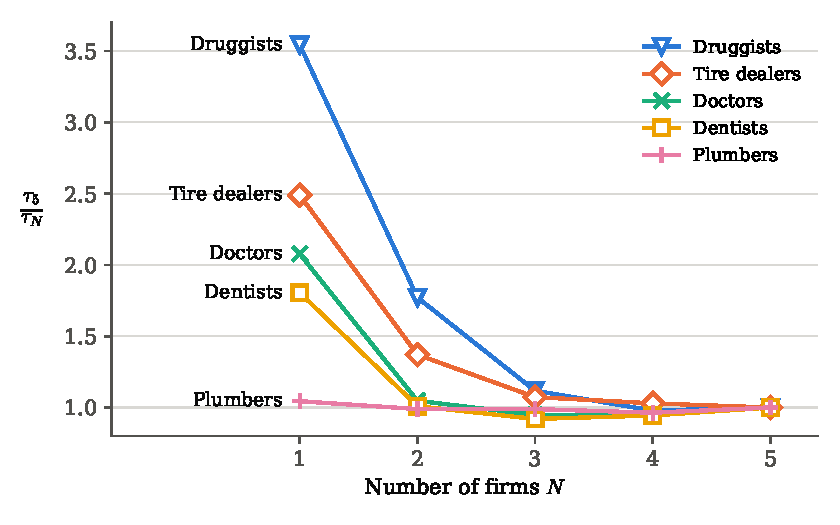
\includegraphics[width=0.82\textwidth]{figures/ch01/br_threshold_ratios.pdf}
\caption{Ratio of the per-firm threshold for five firms to the per-firm threshold for $N$ firms,
$\frac{\tau_5}{\tau_N}$, by industry. A value near one means that the $N$-th firm needs about as many customers
as the fifth. From $N = 3$ on, the ratios lie between 0.92 and 1.12 in every industry. Redrawn from the thresholds in \cref{tab:01-br-thresholds}. Source: Bresnahan and Reiss (1991),
Figure~4 (working-paper version).}
\label{fig:01-br-ratios}
\end{figure}

\casehead{Robustness}
Using ``four or more firms'' as the top category extends the analysis to eight industries. The thresholds of
the original five change little, and heating contractors and barbers show the same pattern. Auto dealers are
the exception, with a per-firm ratio for the fourth dealer well above one (working paper, pp.~18--19). The authors attribute this to product differentiation. Most dealer triopolies pit the three
domestic manufacturers against one another, and the fourth dealer is typically the first intrabrand
competitor. The hypothesis of equal fixed costs across entrants is rejected for every industry except
plumbers, but imposing it barely moves the thresholds. Restricting the sample to very isolated markets, at least 40 miles
from the next town of 1,000 people, leaves 157 markets and similar ratios.
Treating every county with fewer than 10,000 residents in 1980 as a market, isolated or not, sharply reduces
the estimated effect of the second and third doctors and dentists. This is what we would expect if customers
in less isolated towns shop elsewhere, and it supports the strict market definition.

\casehead{Interpretation}
Under the maintained hypotheses that firms in each industry offer similar services with similar technologies
and costs, the results say that entry beyond the third firm changes margins very little. Most of the
competitive effect of entry is felt in highly concentrated markets, with the second and third entrants. The
authors were surprised. They had expected margins, or entry barriers, to erode gradually. Through the lens of
\cref{ex:01-cournot-thresholds} the pattern is sharper than linear Cournot competition implies. Cournot
predicts a second-firm ratio of $1.125$ and ratios above one for every later entrant. Four of the industries
instead show second-firm ratios between 1.78 and 1.99, and every industry shows ratios close to one from the
fourth firm on. In the words of Einav and Levin, competition
appears to ``kick in relatively quickly'' with just a few firms and then does not ramp up with further entry
(p.~155).

\casehead{Critiques}
Bresnahan and Reiss list the main caveats themselves. Without prices, quantities and the timing of entry, they
cannot say whether markets with three or more firms are competitive, only that conduct stops changing
(\cref{rem:01-etr-meaning}). Ratios above one can reflect costlier later entrants as well as falling margins
(\cref{rem:01-etr-costs}). Professionals with low opportunity costs might seek out isolated monopolies, which
would raise the monopoly ratios for reasons unrelated to competition. Einav and Levin add a critique of the
literature that followed (pp.~155--156). One might have expected researchers to look for other identifying
variation, such as differences in fixed costs or entry restrictions, or to gather data on prices and costs.
Instead, most follow-up work developed econometric methods that allow firm heterogeneity or relax parametric
restrictions \citep{Berry1992,BerryTamer2006}, often applying the original identifying assumptions where they
are less compelling. This produced a rich literature on identification and estimation that has not
necessarily brought us closer to the original question.

\casehead{Contribution}
The paper shows how sparse data, used with theory and a clean design, can answer an important question. Counts
of firms in markets of different sizes reveal how competition varies with the number of firms. The entry model
gets around missing data on prices and quantities, which is one reason it has been so influential (p.~160). It
also reframes the SCP question. Concentration is treated as an equilibrium outcome driven by an exogenous
shifter, market size, and the relation between the two identifies how conduct changes with structure.

\begin{remark}[Market size and concentration]\label{rem:01-sutton}
If the per-firm thresholds converge to a finite limit $\tau_\infty$, concentration vanishes in large markets.
Because $\tau_N$ is nondecreasing, $M < M^*_{N^*+1} = (N^* + 1)\tau_{N^*+1} \le (N^* + 1)\tau_\infty$ by
\cref{prop:01-entry-thresholds}(iii). Hence $N^* > \frac{M}{\tau_\infty} - 1$, which grows without bound with
$M$. This argument treats fixed costs as exogenous. \citet{Sutton1991} shows that the conclusion fails when
firms can raise demand through sunk outlays such as advertising or research and development. Such
endogenous sunk costs escalate with market size, and concentration can stay bounded away from zero
however large the market becomes.
\end{remark}

\subsubsection{Industry dynamics}

Many questions about market structure are dynamic \citep[p.~156]{EinavLevin2010}. Do new industries follow a
common life cycle of entry and consolidation? How do firm and industry growth vary with market
characteristics? Are mergers followed quickly by entry, and how do industries adapt to booms and recessions?
A dynamic view can also temper static intuition. Higher concentration reduces static welfare, but the prospect
of market power can create strong incentives to innovate.

The literature has two strands (p.~156). The first looks across industries for robust patterns of survival,
turnover and growth. Its main finding is the large heterogeneity across establishments even within narrow
industries. This finding shaped theoretical models of industry dynamics \citep{Hopenhayn1992}, which in turn
inspired work on firm heterogeneity in international trade \citep{Melitz2003}. The link between entry, exit and
firm characteristics also entered the study of productivity through \citet{OlleyPakes1996}. The second strand
builds models of dynamic equilibrium in single industries, often in the framework of \citet{EricsonPakes1995}.
\citet{Benkard2004} applies such a model to commercial aircraft, where learning by doing lowers costs
dramatically. Equilibrium prices can lie below marginal cost early in a product's life, because extra output
speeds learning. The prospect of market power is what motivates firms to move down the learning curve.
Consumers gain from lower prices both early on and later, when costs are lower. Newer methods estimate sunk
costs, learning and adjustment frictions from panel data on firms or local markets
\citep{AguirregabiriaMira2007,BajariBenkardLevin2007,PakesOstrovskyBerry2007}. \citet{AguirregabiriaCollardWexlerRyan2021}
survey this work in Volume~4 of the Handbook of Industrial Organization. Their chapter lays out the Markov
perfect equilibrium framework, the data typically available, identification and estimation, and applications to
innovation, mergers, regulation, investment, advertising and dynamic pricing \citep[Preface, pp.~xvi--xvii]{HoHortacsuLizzeri2021}.

\begin{remark}[Why learning can push prices below marginal cost]\label{rem:01-learning}
A two-period monopolist faces demand $Q(p)$ in each period and discounts the future by a factor $\delta$. The
first-period cost is $c_1$. Learning makes the second-period cost $c_2(Q_1)$ fall with first-period output,
so $c_2' < 0$. Let $\pi_2(c_2)$ be the optimal second-period profit. By the envelope theorem
$\pi_2'(c_2) = -q_2$, where $q_2$ is second-period output. The firm chooses $p_1$ to maximize
$(p_1 - c_1)Q(p_1) + \delta\,\pi_2\big(c_2(Q(p_1))\big)$. The first-order condition is
\[
  Q(p_1) + (p_1 - c_1)Q'(p_1) + \delta\,\pi_2'(c_2)\,c_2'(Q_1)\,Q'(p_1) = 0 .
\]
Substituting $\pi_2' = -q_2$ and dividing by $-Q'(p_1) > 0$ gives
\[
  p_1 = \big(c_1 - \delta q_2 \lvert c_2' \rvert\big) - \frac{Q(p_1)}{Q'(p_1)} .
\]
The firm prices off an effective marginal cost that is lower than $c_1$ by the discounted value of learning. If
learning is strong enough, $p_1 < c_1$.
\end{remark}

The data available for such models often pale in comparison with the ambitious questions asked, so researchers
fill the gaps with strong assumptions (p.~156). Einav and Levin view this work as ``a quantitative theory
exercise'' (pp.~156--157). It sheds light on dynamic competition in a model with reasonable parameter values.
They do not see this as a problem. It is hard to imagine a clean research design that could pin down the
long-run effect on innovation of a change in the patent system. When the entire history of an industry is a
single data point, quasi-experimental variation is rare, and models are the only way to study such
questions.

\subsection{Structural and design-based approaches}\label{sec:01-today-debate}

Thirty years ago empirical IO resembled other applied fields \citep[p.~157]{EinavLevin2010}. Industrial
organization economists ran cross-industry regressions and faced endogeneity, omitted variables and reverse
causality, much as labor economists running wage regressions did. Since then IO has moved in a distinctive
direction. It turned toward single industries, where measurement and identification are cleaner, and toward
analyses framed by an economic theory of the industry. In the same journal issue, \citet{AngristPischke2010}
describe a parallel move in applied microeconomics toward randomized experiments and quasi-experiments. They
also criticize empirical IO, and Einav and Levin reply. The exchange clarifies the stance of this book.

\subsubsection{Clean measurement versus the object of interest}

No one disagrees about the ideal (p.~157). Every researcher would like to define an object of interest and
then design the perfect experiment to measure it. Without that ideal, researchers face trade-offs, and a
common one is between the cleanness of a measurement and how well the measured object proxies for the object
of interest. Einav and Levin illustrate it with cereal (pp.~157--158). Suppose the object of interest is the
$J \times J$ matrix of price elasticities $E = [\varepsilon_{jk}]$.

\begin{itemize}
  \item The standard IO approach controls for shifts in demand and assumes that the remaining correlation of
        prices across cities reflects costs, as with the Hausman instruments of \citet{Nevo2001}. Within the
        demand model this identifies all of $E$. The assumption may fail.
  \item A design-based alternative looks for an episode that moved one price for an explicable and plausibly
        exogenous reason. An example would be a week in which the pricing algorithm for Froot Loops
        malfunctioned and produced an unintended sale. Such an episode credibly identifies one column of
        $E$, the responses $\varepsilon_{j,\mathrm{FL}}$ of all products to the price of Froot Loops. To learn
        the rest of $E$ we must extrapolate, for instance by assuming that a change in the price of Frosted
        Flakes, or of any cereal, would have analogous effects.
\end{itemize}

Neither approach is ideal. The first relies on a questionable identifying assumption but frames the exercise
directly in terms of the object of interest. The second measures a few entries convincingly but reaches the
object of interest only through a questionable extrapolation. Einav and Levin argue that evaluating entire
research approaches in the abstract paints too simple a picture (p.~158). The right resolution depends on the
question, the data and how compelling a rationale theory provides for the assumptions. There is room for many
approaches, even to the same question, and careful work from different angles is often complementary.

\subsubsection{Theory, transparency and mechanisms}

Angrist and Pischke favor measurement strategies uncontaminated by restrictions from an economic model, partly
on grounds of transparency. Einav and Levin call the implied link between theory and obscurity ``a false
equivalence'' (p.~158). A model derived from theory can be exposited with perfect clarity, and a linear
regression can be exposited with perfect obscurity. It is more natural to start with a research question and
ask how much theory can say about it. Standard theory says little about student behavior in third-grade
classrooms, the setting of Angrist and Pischke's class-size example. There a statistical approach that exploits
variation across thousands of roughly parallel classrooms is attractive. Industrial organization is largely
about firms and markets, which is the other side of the contrast quoted in \cref{sec:01-what-is-io}
(pp.~158--159). Moreover, the interesting question is often a mechanism rather than a single
causal effect. Markets differ greatly, so importing particular numbers across markets is rarely compelling.
Empirical work generalizes best by building support for principles of strategic interaction and market
functioning that apply across industries.

\subsubsection{The merger example}

Angrist and Pischke chose merger evaluation as their example. They dismiss merger simulation as needlessly
indirect and ask why there has not been more retrospective analysis of past mergers. Einav and Levin answer
that the point is good at one level and misses the point at another (p.~159). If the Department of Justice had
to review a merger of Microsoft and Yahoo!, the price effects of past airline or office-supply mergers would be
of little use. It is far more useful to lay out a clear framework for the potential effects of that merger and
to add the best available evidence. \Cref{ch:mergers} presents retrospective studies and merger simulations
side by side, and it shows how each disciplines the other.

The bottom line is that economic theory and the search for compelling identifying variation are allies
(p.~159). The applied work that Einav and Levin find most exciting rests on careful measurement from data with
good variation and then frames the analysis in a coherent economic model. The model gives a way to think about
how the industry works and, potentially, to draw conclusions about policy or general principles. The case
studies of this book are chosen and presented with that standard in mind.

\subsubsection{Methods, applications and the questions IO asks}

Einav and Levin also voice concerns about the field itself (pp.~159--160). Their main concern is that too
little effort goes into compelling applications relative to new econometric methods. Better methods are
valuable if they are eventually used in compelling ways and do not become an end in themselves. In demand
estimation, researchers may have tolerated imperfect price variation because the main contribution was a
method that applies more broadly. Data limitations explain part of the current balance. Some of the most
influential methods were responses to scarce data. The entry model of \citet{BresnahanReiss1991} gets around
missing data on prices and quantities, and the demand model of \citet{BerryLevinsohnPakes1995} needs only
market-level data. As firms collect vast amounts of data on customers, prices, quantities and locations,
richer data may substitute for methods and shift effort toward applications.

A related danger applies to all empirical strategies: the elegance of a solution can pull researchers toward
less important questions (p.~160). Einav and Levin use eBay as an example. Viewed as a laboratory for elegant
auction methods, eBay invites the study of ever narrower submarkets. Broader questions, such as why eBay
succeeded as an institution or how it competes with Amazon and other platforms, would then go unasked.
Researchers should ``resist the temptation of grabbing a hammer and letting it pull them toward a limited set
of nails'' (p.~160).

The last concern is about scope. Schmalensee's review of the cross-industry literature concluded that it had
taught us little about how markets work (\cref{sec:01-scp-today}). After two decades of industry studies, we know a
lot about specific industries such as automobiles, airlines, electricity, and cement and concrete. This
knowledge is extremely disaggregated and does not easily accumulate across industries. As a result, IO has
ceded many important questions about the overall organization of production to trade and macroeconomics.
Einav and Levin suggest that ``it may be time to reclaim them'' (p.~160). The debate over rising markups in
\cref{sec:01-rising-markups} is one place where IO economists are doing so, and it shows how hard the
cross-industry questions remain.

\section{Roadmap of the book}\label{sec:01-roadmap}

The book has four parts and three appendices. Every chapter follows the order of this introduction: theory in
general form first, then case studies that show how the theory meets data. \Cref{tab:01-roadmap} lists, for
each chapter, its central question, its main models and tools, and the papers it treats as full case studies.
Readings that are not case studies receive shorter treatments in the same chapters.

\subsection{The four parts}

Part~I treats market power, its theory and its measurement. This chapter introduced the questions, the SCP
tradition and its failure, the NEIO response and the structural workflow. \Cref{ch:theory} develops the theory that the
rest of the book uses. It covers monopoly pricing, Cournot and Bertrand competition, conjectural variations and
the conduct parameter, pass-through and welfare. \Cref{ch:conduct} asks whether market power can be detected
and measured in homogeneous-good industries. It covers tax pass-through tests, the Panzar-Rosse statistic,
residual demand, the identification of conduct by demand rotations, and direct validations against cost data.
\Cref{ch:diffprod} turns to differentiated products. It derives multi-product Bertrand pricing and diversion
ratios, discusses existence and uniqueness of equilibrium, and contrasts product space with characteristic
space.

Part~II is about demand estimation. \Cref{ch:aids} estimates demand in product space with the Almost Ideal
Demand System, multi-stage budgeting and Hausman instruments. \Cref{ch:discrete} builds the foundations of
discrete choice, including the vertical model and the pure characteristics model. \Cref{ch:logit} covers the
logit and nested logit, the Berry inversion and instruments for price. \Cref{ch:blp} develops the random
coefficients logit of Berry, Levinsohn and Pakes, its estimation and its supply side. \Cref{ch:airlines}
applies these tools to airline hubs and entry. \Cref{ch:newgoods} measures the value of new goods and the bias
in price indexes that ignore them.

Part~III is about competition policy. \Cref{ch:mergers} covers horizontal mergers. It treats market
definition, the theory of mergers in Cournot and differentiated-product models, upward pricing pressure,
merger simulation and retrospective studies. \Cref{ch:collusion-theory} develops the theory of collusion in
repeated games, with demand fluctuations, imperfect monitoring, private information and communication.
\Cref{ch:collusion-evidence} studies how real cartels operated and how collusion can be detected in prices and
bids.

Part~IV is about auctions. \Cref{ch:auction-theory} develops the theory of single-object auctions, from
independent private values to the affiliated values model of Milgrom and Weber. \Cref{ch:auction-empirics}
asks what bid data reveal about values and costs. It covers identification, the estimator of Guerre, Perrigne
and Vuong, unobserved heterogeneity and entry.

Three appendices support the main text. \Cref{app:econometrics} collects the econometric tools: instrumental variables, the
generalized method of moments, maximum likelihood and simulation estimators, the delta method, nonparametric
estimation, and event studies. \Cref{app:math} collects the mathematical tools: the envelope and implicit
function theorems, duality, extreme value algebra, order statistics, contraction mappings, log-concavity and
affiliation. \Cref{app:problems} contains worked problems with full solutions. Two simulated markets recur
there as running examples. One has 25 logit products sold by five owners. The other has 100 markets drawn from a pool of ten
products, and each market offers between four and nine of them. It is generated from a random-coefficients logit
with a cost shifter, and on it the vertical, logit and random-coefficients estimators are compared.

\begin{table}[htbp]
\centering
\caption{Roadmap of the book}
\label{tab:01-roadmap}
\scriptsize
\renewcommand{\arraystretch}{1.0}
\begin{tabularx}{\textwidth}{@{}>{\raggedright\arraybackslash}p{1.95cm}
  >{\raggedright\arraybackslash}X >{\raggedright\arraybackslash}X >{\raggedright\arraybackslash}X@{}}
\toprule
Chapter & Central question & Main models and tools & Case studies in depth \\
\midrule
\multicolumn{4}{@{}l}{\textit{Part I. Market power: theory and measurement}} \\
\ref{ch:intro}. Introduction & How do we learn about market power and its causes? & SCP regressions, the
  Cournot link between margins and concentration, the conduct parameter, the structural workflow &
  \citet{BresnahanReiss1991}, \citet{GriecoMurryYurukoglu2024} (and substantive treatments of
  \citet{Bresnahan1989} and \citet{EinavLevin2010}) \\
\ref{ch:theory}. Pricing theory & How do demand, cost and conduct determine prices? & Monopoly pricing,
  Cournot and Bertrand oligopoly, conjectural variations, pass-through, welfare & None \\
\ref{ch:conduct}. Measuring market power & Can we detect and measure market power with homogeneous goods? &
  Tax pass-through tests, Panzar-Rosse statistic, residual demand, identification of conduct by rotations &
  \citet{Sumner1981}, \citet{Corts1999}, \citet{GenesoveMullin1998}, \citet{Wolfram1999} \\
\ref{ch:diffprod}. Differentiated oligopoly & How do multi-product firms price differentiated goods? &
  Multi-product Bertrand-Nash pricing, ownership matrix, diversion ratios, existence and uniqueness, location
  models & None \\
\addlinespace
\multicolumn{4}{@{}l}{\textit{Part II. Demand estimation}} \\
\ref{ch:aids}. AIDS & How do we estimate flexible demand in product space? & Duality, AIDS, multi-stage
  budgeting, Hausman instruments, welfare & \citet{DeatonMuellbauer1980a}, \citet{HausmanLeonardZona1994},
  \citet{ChaudhuriGoldbergJia2006} \\
\ref{ch:discrete}. Discrete choice & How do individual choices aggregate to market demand? & Random utility,
  vertical model, pure characteristics model, hedonic approach & \citet{Bresnahan1987},
  \citet{BerryPakes2007} \\
\ref{ch:logit}. Logit & How do we estimate logit demand with endogenous prices? & Logit, Berry inversion,
  instruments, nested logit & \citet{Berry1994}, \citet{Einav2007}, \citet{Hendel1999} \\
\ref{ch:blp}. BLP & How do we obtain realistic substitution from market-level data? & Random coefficients
  logit, contraction mapping, GMM, supply side, micro moments & \citet{BerryLevinsohnPakes1995},
  \citet{Nevo2000a}, \citet{Nevo2001}, \citet{BerryLevinsohnPakes2004}, \citet{Goldberg1995} \\
\ref{ch:airlines}. Airlines & Why are fares high at hubs, and how does entry discipline them? & Fare
  regressions, event studies, discrete choice with consumer types and hub costs & \citet{Borenstein1989},
  \citet{WhinstonCollins1992}, \citet{BerryCarnallSpiller2006} \\
\ref{ch:newgoods}. New goods & What is a new good worth to consumers? & Virtual prices, compensating variation,
  logit welfare, micro moments & \citet{Hausman1997}, with the comment by \citet{Bresnahan1997};
  \citet{Trajtenberg1989}, \citet{Petrin2002}, \citet{Gentzkow2007} \\
\addlinespace
\multicolumn{4}{@{}l}{\textit{Part III. Competition policy}} \\
\ref{ch:mergers}. Mergers & When do horizontal mergers raise prices? & Market definition, Cournot merger
  analysis, upward pricing pressure, merger simulation, retrospectives & \citet{FarrellShapiro1990},
  \citet{FarrellShapiro2010}, \citet{Nevo2000b}, \citet{BjornerstedtVerboven2016},
  \citet{MillerWeinberg2017} \\
\ref{ch:collusion-theory}. Collusion: theory & How can firms sustain collusion without enforceable contracts? &
  Repeated games, optimal punishments, demand fluctuations, imperfect monitoring, private information,
  communication & \citet{GreenPorter1984}, \citet{RotembergSaloner1986},
  \citet{AtheyBagwellSanchirico2004}, \citet{HarringtonSkrzypacz2011} \\
\ref{ch:collusion-evidence}. Collusion: evidence & How did cartels operate, and how can we detect them? &
  Regime-switching supply relations, tests of price-war theories, bidding rings, tests for bid rigging &
  \citet{Porter1983}, \citet{Ellison1994}, \citet{PorterZona1993}, \citet{Asker2010} \\
\addlinespace
\multicolumn{4}{@{}l}{\textit{Part IV. Auctions}} \\
\ref{ch:auction-theory}. Auction theory & How do rules and information shape bids and revenue? & Private and
  affiliated values, first- and second-price equilibrium, revenue equivalence, reserve prices, linkage
  principle & \citet{MilgromWeber1982} \\
\ref{ch:auction-empirics}. Auction empirics & What do bids reveal about values and costs? & Order-statistic
  inversion, the GPV estimator, unobserved heterogeneity, entry, timber auctions &
  \citet{AtheyHaile2002}, \citet{AtheyHaile2007}, \citet{GuerrePerrigneVuong2000},
  \citet{Krasnokutskaya2011}, \citet{AtheyLevinSeira2011} \\
\bottomrule
\end{tabularx}
\par\smallskip
\begin{minipage}{\textwidth}\footnotesize
\textit{Notes:} The last column lists the papers treated as full case studies, following the structure
described in \cref{sec:01-roadmap-conventions}. Each chapter also gives shorter treatments of the other
readings in its scope.
\end{minipage}
\end{table}

\subsection{Reading paths}

The chapters build on one another, but several shorter paths through the book work well.
\begin{itemize}
  \item A reader interested in antitrust and merger analysis can read
        \cref{ch:theory,ch:conduct,ch:diffprod,ch:logit,ch:blp,ch:mergers}. This path runs from pricing
        theory and the measurement of market power to the demand models that merger simulation requires.
  \item A reader interested in demand estimation can read
        \cref{ch:aids,ch:discrete,ch:logit,ch:blp,ch:airlines,ch:newgoods}, after \cref{sec:01-workflow} and
        the multi-product pricing of \cref{ch:diffprod}.
  \item A reader interested in collusion can read
        \cref{ch:theory,ch:conduct,ch:collusion-theory,ch:collusion-evidence}.
  \item A reader interested in auctions can read \cref{ch:auction-theory,ch:auction-empirics}, after
        \cref{sec:01-today-auctions}. The bid-rigging material of \cref{ch:collusion-evidence} is a natural
        complement.
\end{itemize}

\subsection{Prerequisites and conventions}\label{sec:01-roadmap-conventions}

We assume graduate training in microeconomic theory and econometrics. On the theory side the reader should
know consumer theory and duality, and Nash, subgame perfect and Bayesian Nash equilibrium. On the econometric
side the reader should know least squares, instrumental variables, the generalized method of moments and
maximum likelihood. \Cref{app:econometrics,app:math} fill gaps. For the theory of industrial organization at
greater length, \citet{Tirole1988} remains the standard reference. For surveys of recent work, including topics
outside this edition, the reader can turn to Volumes~4 and~5 of the Handbook of Industrial Organization
\citep{HoHortacsuLizzeri2021a,HoHortacsuLizzeri2021}. Their Preface describes every chapter
\citep[pp.~xv--xxi]{HoHortacsuLizzeri2021}. The first five chapters review econometric methods that continue the
NEIO program, Chapters~6 to~9 review theory, and Chapters~10 to~17 apply both to policy questions and to
particular sectors. \Cref{tab:01-handbook} lists the chapters and the parts of this book that each one extends.

\begin{table}[htbp]
\centering
\caption{The chapters of the Handbook of Industrial Organization, Volumes 4 and 5}
\label{tab:01-handbook}
\footnotesize
\renewcommand{\arraystretch}{1.08}
\begin{tabularx}{\textwidth}{@{}>{\raggedright\arraybackslash}p{1.1cm}
  >{\raggedright\arraybackslash}p{4.4cm} >{\raggedright\arraybackslash}X >{\raggedright\arraybackslash}p{3.3cm}@{}}
\toprule
Chapter & Authors & Topic & Extends \\
\midrule
\multicolumn{4}{@{}l}{\textit{Volume 4: econometric methods (Chapters 1 to 5) and theory (Chapters 6 to 9)}} \\
1 & Berry and Haile & Foundations of demand estimation & \cref{ch:discrete,ch:logit,ch:blp} \\
2 & Gandhi and Nevo & Demand and supply in differentiated-products industries, opening with
  \citet{Bresnahan1987} & \cref{ch:discrete,ch:blp,ch:mergers} \\
3 & De Loecker and Syverson & Productivity, and the production approach to market power &
  \cref{sec:01-rising-markups} \\
4 & Aguirregabiria, Collard-Wexler and Ryan & Dynamic games & \cref{sec:01-today-structure} \\
5 & Kline, Pakes and Tamer & Moment inequalities and partial identification & \cref{sec:01-today-structure} \\
6 & Gavazza and Lizzeri & Frictions in product markets & Not covered \\
7 & Jullien, Pavan and Rysman & Two-sided markets, pricing and network effects & \cref{sec:01-early-studies} \\
8 & Bergemann and Ottaviani & Information markets and nonmarkets & Not covered \\
9 & Lee, Whinston and Yurukoglu & Contracting in vertical markets & Not covered \\
\addlinespace
\multicolumn{4}{@{}l}{\textit{Volume 5: applications to policy questions and sectors}} \\
10 & Agarwal and Budish & Market design & \cref{ch:auction-theory} \\
11 & Horta{\c{c}}su and Perrigne & Empirical perspectives on auctions & \cref{ch:auction-empirics} \\
12 & Asker and Nocke & Collusion, mergers and related antitrust issues &
  \cref{ch:mergers,ch:collusion-theory,ch:collusion-evidence} \\
13 & Bryan and Williams & Innovation: market failures and public policies & Not covered \\
14 & Einav, Finkelstein and Mahoney & Selection markets & \cref{sec:01-today-pricing} \\
15 & Clark, Houde and Kastl & Financial markets & Not covered \\
16 & Handel and Ho & Health care markets & \cref{sec:01-scp-today} \\
17 & Kellogg and Reguant & Energy and environmental markets & \cref{sec:01-today-auctions} \\
\bottomrule
\end{tabularx}
\par\smallskip
\begin{minipage}{\textwidth}\footnotesize
\textit{Notes:} Chapter titles are abbreviated. ``Extends'' names the chapter or section of this book that the
Handbook chapter continues. Source: \citet[Preface, pp.~xv--xxi]{HoHortacsuLizzeri2021}.
\end{minipage}
\end{table}

Notation is fixed across chapters. Markets are indexed by $t$ and products by $j$, with $j = 0$ the outside
good. Firms are indexed by $f$ in differentiated-product models and by $i$ in homogeneous-good models, and
consumers by $i$ in discrete choice models. Market shares are $s_{jt}$, marginal costs $mc_{jt}$, the price elasticity of demand
$\varepsilon > 0$, the conduct parameter $\theta$ and the ownership matrix $\Omega$. Mean utility is
$\delta_{jt} = x_{jt}\beta - \alpha p_{jt} + \xi_{jt}$, and auctions use $v$ for values, $b$ for bids and $G$
for the distribution of bids. When a chapter must depart from this notation, or rename the symbols of a paper,
it says so at first use.

Each case study follows the same order. We state the economic question and why it matters, the institutional
setting and the data. We then write the model and the exact estimating equations, the estimator, the
instruments and the identification argument. We reproduce the key results in a table, citing the table number
in the original paper, and discuss robustness, interpretation, the critiques raised in the literature and the
paper's contribution. Every chapter ends with exercises and with bibliographic notes that place its papers in
context.


\section{Bibliographic notes}\label{sec:01-bibnotes}

The structure-conduct-performance tradition begins with \citet{Mason1939} and the cross-industry studies of
\citet{Bain1951,Bain1956}. The Introduction of \citet{Tirole1988} tells its history, together with the Chicago
tradition and the theoretical wave that followed \citep{Joskow1975}. \citet{Schmalensee1989} is the standard
review of its evidence, and \citet{Weiss1989} collects the price-concentration studies of local markets.
\citet{Demsetz1973} stated the efficiency critique, and \citet{Schmalensee1987} tests it against the collusion
hypothesis. \citet{Hopenhayn1992} shows that high entry costs can produce the pattern Demsetz reported in a
competitive model, and
\citet{LevensteinSuslow2006} place the debate within the study of cartels. \citet{Salinger1990} revisited the debate with a panel of
industries, using annual cross sections and long differences. The measurement problems of accounting margins are analyzed by
\citet{FisherMcGowan1983}. The Cournot foundation of the margin-concentration relation is due to
\citet{CowlingWaterson1976}, with the conduct generalization of \citet{ClarkeDavies1982}. Section~5.5 of
\citet{Tirole1988} links concentration indices to industry profitability, and \citet{EncaouaJacquemin1980} give
the axioms that define them.

The New Empirical Industrial Organization is surveyed by \citet{Bresnahan1989}, whose chapter remains the best
statement of its principles and of its identification arguments. Its antecedents include \citet{Rosse1970}, and
its central identification results are \citet{Bresnahan1982} and \citet{Lau1982} for demand rotations and
\citet{PanzarRosse1987} for comparative statics in cost. \citet{Porter1983} is the classic application to a
cartel. \Cref{ch:conduct} develops these results, the tax tests of \citet{Sumner1981} and
\citet{AshenfelterSullivan1987}, and the critique by \citet{Corts1999}.

Modern empirical IO is surveyed by \citet{EinavLevin2010}. Volumes~4 and~5 of the Handbook of Industrial
Organization \citep{HoHortacsuLizzeri2021a,HoHortacsuLizzeri2021} survey its methods and applications chapter by
chapter, and \cref{tab:01-handbook} maps each chapter to this book. Among them, \citet{DeLoeckerSyverson2021} treat
productivity and the production approach to markups, and \citet{AguirregabiriaCollardWexlerRyan2021} treat dynamic
games. \citet{AskerNocke2021} cover collusion and mergers, and \citet{HandelHo2021} cover health care. \citet{Tirole1988} remains the
standard treatment of the theory. The demand models behind the structural workflow start with \citet{Berry1994} and
\citet{BerryLevinsohnPakes1995}, and the parallel approach to auctions starts with \citet{GuerrePerrigneVuong2000}.
\citet{BresnahanReiss1991} is the founding paper of the empirical entry literature, and \citet{Sutton1991} gives
the theory of endogenous sunk costs.

The debate over rising markups starts with \citet{DeLoeckerEeckhoutUnger2020}, who build on the production
approach of \citet{Hall1988} and \citet{DeLoeckerWarzynski2012}. Section~3.8 of \citet{AskerNocke2021}
summarizes their findings and the measurement questions they raise, and \citet{Ganapati2020} documents how
concentration relates to productivity, output and prices. \citet{BerryGaynorScottMorton2019} give the IO
perspective on that debate, which \citet{HandelHo2021} apply to health care and \citet{AutorEtAl2020} connect to
the labor share. \citet{BondEtAl2021} analyze the use of revenue data. \citet{GriecoMurryYurukoglu2024} study one
industry from the demand side and find that markups in the US new-car market fell after 1980 while consumer
surplus rose. The exchange between
\citet{AngristPischke2010} and \citet{EinavLevin2010} sets out the case for and against structural models in
applied microeconomics.

\section{Exercises}\label{sec:01-exercises}

\begin{enumerate}[label=\arabic*., leftmargin=*, itemsep=6pt]

\item \textit{Measuring the market power of one seller.} A coffee shop on a university campus sets a single price
for a cup of coffee.
\begin{enumerate}[label=(\alph*)]
  \item Describe the data and the variation in prices you would need to estimate the elasticity of the shop's
  residual demand. Explain why a regression of its daily sales on its daily price would not, in general, estimate
  that elasticity.
  \item Suppose you have such an estimate. Explain what you could conclude about marginal cost from
  \cref{prop:01-infer-cost}, and which maintained assumption the conclusion rests on.
  \item Consider three events: a per-unit tax on coffee sold on campus, a rise in the world price of coffee beans,
  and the opening of a rival cafe in the same building. For each event, say which primitive (demand, cost or
  conduct) it moves. Then explain what the observed response of price would reveal.
  \item Suppose the shop is the monopolist of \cref{ex:01-quality-markup}, with $\alpha = 0.5$ per dollar and a
  share $s = 0.4$ of potential customers. It improves its coffee at no change in marginal cost. Compute the change
  in price and in net utility $v$ per unit of quality. Explain why a regulator who saw the Lerner index rise would
  be wrong to conclude that customers lost.
\end{enumerate}

\item \textit{Concentration and mergers.}
\begin{enumerate}[label=(\alph*)]
  \item Construct two share vectors with the same four-firm concentration ratio $\mathit{CR}_4$ and different
  Herfindahl indices, and two with the same Herfindahl index and different $\mathit{CR}_4$. Compute the numbers
  equivalent $N^{\mathrm{eq}}$ of each.
  \item Firms $i$ and $j$ merge, and the merged firm keeps the share $s_i + s_j$. Show that the merger lowers the
  numbers equivalent from $\frac{1}{\HHI}$ to $\frac{1}{\HHI + 2 s_i s_j}$, and compute both for $s_i = 0.2$,
  $s_j = 0.1$ and $\HHI = 0.15$.
  \item Consider symmetric Cournot competition with linear demand among four firms with equal constant marginal
  costs. Two firms merge, and the merged firm has the same marginal cost as before. Compute the predicted change
  in the Herfindahl index from part (b) and the actual change in the new Cournot equilibrium. Explain the
  difference.
  \item Show that the entropy index $\sum_i s_i \ln s_i$ rises when share moves from a smaller to a larger
  firm, as \cref{rem:01-ej-axioms} requires. Then construct a transfer between two firms that leaves
  $\mathit{CR}_4$ unchanged and raises $\HHI$.
\end{enumerate}

\item \textit{Conduct and the slope of the SCP regression.} Industries $k = 1, \dots, n$ share a common market
elasticity $\varepsilon$. Each industry is either Cournot ($\kappa_k = 0$) or perfectly collusive
($\kappa_k = 1$), so that by \cref{prop:01-clarke-davies} its margin is
$L_k = \frac{\kappa_k + (1 - \kappa_k)\HHI_k}{\varepsilon}$.
\begin{enumerate}[label=(\alph*)]
  \item Suppose $\HHI_k$ is uniform on $[0, 1]$ and $\Pr(\kappa_k = 1 \mid \HHI_k = h) = 1 - h$, because collusive
  industries attract entry. Use \cref{prop:01-scp-plim}(i) to compute the probability limit of the OLS slope of
  $L_k$ on $\HHI_k$.
  \item Compare your answer with $\E\left[\frac{1 - \kappa_k}{\varepsilon}\right]$, the slope that random
  assignment of concentration would deliver. Explain the sign of the bias.
  \item The regression in (a) suggests that concentration does not affect margins. Yet the margin of every
  Cournot industry rises with concentration at the rate $\frac{1}{\varepsilon}$. Explain the discrepancy.
\end{enumerate}

\item \textit{Free entry and the cross-industry correlation.} Use the free-entry Cournot model of
\cref{sec:01-endogeneity} with a continuous number of firms.
\begin{enumerate}[label=(\alph*)]
  \item Derive $N^*$, $\HHI^*$ and $L^*$ as functions of $(a, c, b, F)$.
  \item Compute the equilibrium for four industries: $(a, c, b, F) = (10, 2, 1, 1)$, $(10, 2, 1, 4)$, $(10, 4, 1, 1)$
  and $(14, 2, 1, 1)$.
  \item Pair the first industry with each of the other three. For each pair, compute the slope of the line through
  the two points $(\HHI^*, L^*)$. Compare these slopes with the slope $\frac{\dd L}{\dd \HHI}$ of each industry's own
  causal curve \eqref{eq:01-linear-cournot-LH} at its equilibrium. Which pairs, if any, reveal a causal effect of
  concentration?
\end{enumerate}

\item \textit{Efficiency and concentration.} Inverse demand is $P = 10 - Q$, and three Cournot firms have
marginal costs $(2, 3, 4)$.
\begin{enumerate}[label=(\alph*)]
  \item Use \cref{prop:01-demsetz} to compute the price, total output, each firm's output and share, the Herfindahl
  index, industry variable profit and consumer surplus.
  \item Replace the costs by $(1.5, 3, 4.5)$. Verify that all firms stay active and recompute every quantity in
  (a). Which change, and by how much does total surplus change?
  \item Return to the costs $(2, 3, 4)$. The two lowest-cost firms merge and produce at the lower of their two
  costs. Compute the new equilibrium. Compare the actual change in the Herfindahl index with the share-based
  prediction $2 s_1 s_2$, and compute the changes in price and consumer surplus.
  \item What do (b) and (c) imply for a regulator who observes only concentration and industry profits?
\end{enumerate}

\item \textit{Measurement error, fixed effects and accounting margins.}
\begin{enumerate}[label=(\alph*)]
  \item Show that the Census price-cost margin equals the Lerner index whenever variable cost (payroll and
  materials) is linear in output, whatever the cost of capital. Derive the probability limit of the OLS slope in a
  regression of $\mathit{PCM}_k$ on $\HHI_k$ that omits $\frac{K_k}{S_k}$, and sign the bias when capital intensity
  rises with concentration.
  \item In the setting of \cref{prop:01-fe-attenuation}, let the total variance of true concentration across
  industry-years be $0.04$, of which 90 percent is between industries, so that $\sigma^2_{\tilde H} = 0.004$. Let
  $\sigma_u^2 = 0.002$ and $T = 5$. Compute the reliability ratio of the pooled OLS estimator and of the within
  estimator, and the probability limit of each when $\beta_1 = 0.5$ and the pooled estimator is otherwise valid.
  \item Explain why the gain from removing industry fixed effects can be smaller than the loss from attenuation.
\end{enumerate}

\item \textit{Identification of conduct in a linear model.} Consider the linear model \eqref{eq:01-linear-id-model}
with supply relation \eqref{eq:01-linear-supply}.
\begin{enumerate}[label=(\alph*)]
  \item Show that a monopoly ($\theta = 1$) with marginal cost slope $b_1$ and a competitive industry ($\theta = 0$)
  with marginal cost slope $b_1 - \frac{1}{a_1}$ generate the same joint distribution of $(P_t, Q_t)$ given
  $(Y_t, W_t)$.
  \item Now let demand be $Q_t = a_0 + (a_1 + a_3 Y_t) P_t + a_2 Y_t + u^d_t$ with $a_3 \ne 0$. Derive the supply
  relation implied by \cref{prop:01-supply-relation}. Show that it contains two regressors, $Q_t$ and
  $\frac{Q_t}{a_1 + a_3 Y_t}$, that are not collinear.
  \item Explain which exogenous variables can serve as instruments for the two regressors in (b), and why the
  argument fails when $a_3 = 0$. Relate your answer to \cref{rem:01-lau}.
\end{enumerate}

\item \textit{Entry thresholds and conduct.} Work under \cref{ass:01-br}.
\begin{enumerate}[label=(\alph*)]
  \item Show that if the $N$ firms in every market collude perfectly, every entry threshold ratio
  $\frac{\tau_{N+1}}{\tau_N}$ equals one. Show that homogeneous Bertrand competition with constant marginal cost
  and $F > 0$ never supports two firms.
  \item In the linear Cournot model of \cref{ex:01-cournot-thresholds}, let the $N$-th entrant pay the fixed cost
  $F_N = F + (N - 1)\Delta$ with $\Delta \ge 0$. Use \cref{rem:01-etr-costs} to compute $\frac{\tau_2}{\tau_1}$,
  and find the ratio $\frac{\Delta}{F}$ that matches the dentist ratio in \cref{tab:01-br-thresholds}.
  \item Use the dentist thresholds in \cref{tab:01-br-thresholds} to compute $\frac{\tau_2}{\tau_1}$ and
  $\frac{\tau_3}{\tau_2}$. Compare them with the linear Cournot ratios. What do they suggest about how competition
  changes with the second and the third dentist?
  \item Explain why per-firm ratios equal to one from the fourth firm on do not show that markets with four or
  more firms are competitive. Which additional data would settle the question?
\end{enumerate}

\end{enumerate}
